\section{Data Sample}
\label{sec:datasampleAndSelection}
The data sample used for this analysis corresponds to 19.7$\pm0.5~\fbinv$ of integrated 
luminosity collected in 2012 at $\sqrt{s} = 8~\TeV$.  See Table \ref{table:datasets} for a summary of the datasets used in the analysis.
Generation of SM $\ttbar$ and single top events is performed by Powheg~\cite{Oleari:2010nx}.  
The MC simulation samples used for background estimation can be found in table \ref{table:datasets}.

\begin{table}
\begin{center}
\bf{Jet Datasets}
\begin{tabular}{p{0.7\linewidth}|c}
\hline\hline
\bf{Dataset} & \bf{Luminosity ($\pbinv$)} \\
\hline\hline
/Jet/Run2012A-22Jan2013-v1/AOD & $888$ \\
/JetHT/Run2012B-22Jan2013-v1/AOD & $4403$ \\
/JetHT/Run2012C-22Jan2013-v1/AOD & $7052$ \\
/JetHT/Run2012D-22Jan2013-v1/AOD & $7414$ \\
Total Analyzed Luminosity & $19757$ \\
\hline 
\\
\\
\end{tabular}
\bf{MC Datasets} \\
\begin{tabular}{p{0.7\linewidth}|c}
\hline\hline
\bf{Dataset} & \bf{Cross-section(pb)} \\
\hline\hline
TT\_Mtt-700to1000\_CT10\_TuneZ2star\_8TeV-powheg-tauola & $245.8$ (NNLO)\\
TT\_Mtt-1000toInf\_CT10\_TuneZ2star\_8TeV-powheg-tauola & $245.8$ (NNLO)\\
T\_t-channel\_TuneZ2star\_8TeV-powheg-tauola & $56.4$ (NNLO)\\
Tbar\_t-channel\_TuneZ2star\_8TeV-powheg-tauola & $30.7$ (NNLO)\\
Tbar\_tW-channel-DR\_TuneZ2star\_8TeV-powheg-tauola & $11.1$ (NNLO)\\
T\_tW-channel-DR\_TuneZ2star\_8TeV-powheg-tauola & $11.1$ (NNLO)\\
T\_s-channel\_TuneZ2star\_8TeV-powheg-tauola & $3.79$ (NNLO)\\
Tbar\_s-channel\_TuneZ2star\_8TeV-powheg-tauola & $1.76$ (NNLO)\\
QCD\_Pt-300to470\_TuneZ2star\_8TeV\_pythia6 & $1759.6$ \\
QCD\_Pt-470to600\_TuneZ2star\_8TeV\_pythia6 & $113.9$ \\
QCD\_Pt-600to800\_TuneZ2star\_8TeV\_pythia6 & $27.0$ \\
QCD\_Pt-800to1000\_TuneZ2star\_8TeV\_pythia6 & $3.57$ \\
QCD\_Pt-1000to1400\_TuneZ2star\_8TeV\_pythia6 & $0.738$ \\
QCD\_Pt-1400to1800\_TuneZ2star\_8TeV\_pythia6 & $0.0335$ \\
\hline

\end{tabular}
\end{center}
\caption{Primary datasets and MC samples used. Including the corresponding integrated luminosity or cross-section of each dataset \cite{Czakon:2013goa,Kidonakis:2012db}.}
\label{table:datasets}
\end{table}

\subsection{Signal Samples}
\label{sec:signal}
The Lagrangian presented in equation \ref{eqn:Lag} has been implemented in CompHEP \cite{CompHEP} and used for event generation.  The mass of the top 
quark was set to 172.5~$\GeV$.  
Pythia was used for hadronization. The CTEQ6M parton distribution functions were selected and the QCD scale was set to the $\wpr$ invariant mass.  The width of 
the $\wpr$ resonance and cross-sections were obtained from CompHEP numerical calculations.  The generation was performed using the 2 $\rightarrow$ 4 
process $\wpr \rightarrow$ t ; t $\rightarrow$ Wb ; W $\rightarrow$ $q_{i}q_{j}$, where $q_{i}$ and $q_{j}$ represent quarks.  
W decays including b quarks are not considered due to the negligible branching fraction.  The process 
preserves all spin correlations between production and decay.

The $\wpr$ generation can be performed using three different couplings. 
\begin{itemize}
\item {\bf $\wpr_{R}$} - The purely right-handed $\wpr$ where $a_{qi,qj}^{L}$=0 , $a_{qi,qj}^{R}$=1 
\item {\bf $\wpr_{L}$} - The purely left-handed $\wpr$ where $a_{qi,qj}^{L}$=1 , $a_{qi,qj}^{R}$=0 
\item {\bf $\wpr_{LR}$} - The mixed-coupling $\wpr$ where $a_{qi,qj}^{L}$=1 , $a_{qi,qj}^{R}$=1 
\end{itemize}

Because of the SM-like couplings of $\wpr_{L}$ and $\wpr_{LR}$, we must consider the 
interference between SM single top and signal.  The $\wpr_{R}$ MC samples were generated without SM single top.  The right-handed $\wpr$ samples used in this analysis are given in table
\ref{table:signalsets}.  The cross-sections listed here are leading order.  The cross-sections 
used in the main analysis are scaled to next-to leading order with a multiplicative k factor of 1.2
which is extracted from \cite{kfactor}.  The left-handed and mixed-coupling $\wpr$ samples used 
in this analysis are given in table \ref{table:signalsetsleft} and \ref{table:signalsetsmixed} respectively.
In order to have sufficient statistical precision in the signal region, these samples have a loose generator 
level $\pt$ cut of 200$~\GeV$ set on the b jet from the $\wpr$ decay.  The effect of this pre-selection is investigated in section \ref{sec:GenBptCut}.

\begin{table}
\begin{center}
\bf{Right-Handed Signal Samples}
\begin{tabular}{p{0.48\linewidth}|c|c}
\hline\hline
\bf{Dataset} & \bf{$\Gamma_{\wpr} (\GeV)$} & \bf{(LO) Cross-Section (pb)} \\
\hline\hline
SingletopWprimeTToHad\_M-1300\_right\_TuneZ2star\_8TeV-comphep & 43.7 & 0.4852 \\
SingletopWprimeTToHad\_M-1500\_right\_TuneZ2star\_8TeV-comphep  & 50.0 & 0.2198 \\
SingletopWprimeTToHad\_M-1700\_right\_TuneZ2star\_8TeV-comphep  & 57.3 & 0.1038 \\
SingletopWprimeTToHad\_M-1900\_right\_TuneZ2star\_8TeV-comphep  & 64.1 & 0.0507 \\
SingletopWprimeTToHad\_M-2100\_right\_TuneZ2star\_8TeV-comphep  & 70.9 & 0.0254 \\
SingletopWprimeTToHad\_M-2300\_right\_TuneZ2star\_8TeV-comphep  & 77.6 & 0.0131 \\
SingletopWprimeTToHad\_M-2700\_right\_TuneZ2star\_8TeV-comphep  & 91.2 & 0.0039 \\
\hline
\end{tabular}
\end{center}
\caption{Signal samples used in the analysis.  Quoted cross-section and $\Gamma_{\wpr}$ were obtained from the CompHEP generator. A k factor of 1.2 is implemented on the quoted cross-sections.}
\label{table:signalsets}
\end{table}


\begin{table}
\begin{center}
\bf{Left-Handed Signal Samples}
\scalebox{0.75}{
\begin{tabular}{p{0.48\linewidth}|c|c|c}
\hline\hline
\bf{Dataset} & \bf{$\Gamma_{\wpr} (\GeV)$} & \bf{(LO) Cross-Section (pb)} & \bf{Selection Efficiency} \\
\hline\hline
SingletopWprimeTToHad\_M-1300\_left\_TuneZ2star\_8TeV-comphep & 43.7 & 0.4248 & 0.157 \\
SingletopWprimeTToHad\_M-1500\_left\_TuneZ2star\_8TeV-comphep  & 50.0 & 0.2622 & 0.104 \\
SingletopWprimeTToHad\_M-1700\_left\_TuneZ2star\_8TeV-comphep  & 57.3 & 0.1669 & 0.0679 \\
SingletopWprimeTToHad\_M-1900\_left\_TuneZ2star\_8TeV-comphep  & 64.1 & 0.1237 & 0.0507 \\
SingletopWprimeTToHad\_M-2100\_left\_TuneZ2star\_8TeV-comphep  & 70.9 & 0.1047 & 0.0429 \\
SingletopWprimeTToHad\_M-2300\_left\_TuneZ2star\_8TeV-comphep  & 77.6 & 0.0971 & 0.0397 \\
SingletopWprimeTToHad\_M-2700\_left\_TuneZ2star\_8TeV-comphep  & 91.2 & 0.0933 & 0.0379 \\
\hline
\end{tabular}
}
\end{center}
\caption{Left-Handed signal samples used in the analysis.  Quoted cross-section and $\Gamma_{\wpr}$ were obtained from the CompHEP generator.  A k factor of 1.2 is implemented on the quoted cross-sections.  The cross sections listed here take into account the generator level b jet $\pt$ cut, and represent the visible cross section.  The efficiency of this cut is provided under the column labeled Selection Efficiency.}
\label{table:signalsetsleft}
\end{table}

\begin{table}
\begin{center}
\bf{Mixed Signal Samples}
\scalebox{0.75}{
\begin{tabular}{p{0.48\linewidth}|c|c|c}
\hline\hline
\bf{Dataset} & \bf{$\Gamma_{\wpr} (\GeV)$} & \bf{(LO) Cross-Section (pb)} & \bf{Selection Efficiency} \\
\hline\hline
SingletopWprimeTToHad\_M-1300\_mixed\_TuneZ2star\_8TeV-comphep & 87.4 & 0.9327 & 0.290 \\
SingletopWprimeTToHad\_M-1500\_mixed\_TuneZ2star\_8TeV-comphep & 101.0 & 0.4743 & 0.172 \\
SingletopWprimeTToHad\_M-1700\_mixed\_TuneZ2star\_8TeV-comphep & 114.6 & 0.2700 & 0.105 \\
SingletopWprimeTToHad\_M-1900\_mixed\_TuneZ2star\_8TeV-comphep & 128.2 & 0.1776 & 0.0711 \\
SingletopWprimeTToHad\_M-2100\_mixed\_TuneZ2star\_8TeV-comphep & 141.7 & 0.1334 & 0.0540 \\
SingletopWprimeTToHad\_M-2300\_mixed\_TuneZ2star\_8TeV-comphep & 155.3 & 0.1128 & 0.0458 \\
SingletopWprimeTToHad\_M-2700\_mixed\_TuneZ2star\_8TeV-comphep & 182.4 & 0.0986 & 0.0400 \\
\hline
\end{tabular}
}
\end{center}
\caption{Mixed-Coupling signal samples used in the analysis.  Quoted cross-section and $\Gamma_{\wpr}$ were obtained from the CompHEP generator.  A k factor of 1.2 is implemented on the quoted cross-sections.  The cross sections listed here take into account the generator level b jet $\pt$ cut, and represent the visible cross section.  The efficiency of this cut is provided under the column labeled Selection Efficiency.}
\label{table:signalsetsmixed}
\end{table}


\subsection{Trigger Selection}
\label{sec:trigger}
Due to our interest in highly boosted jets, our data was taken using the \texttt{HLT\_HT750} trigger, which requires the event to have $\mathrm{H_t}$ of at least 750 $\GeV$. 
The trigger efficiency is measured in data and MC by investigating the looser \texttt{HLT\_HT550} trigger.  The selection used for this measurement includes a loose kinematic selection.  We require two jets 
with $\pt > 300$ $\GeV$ and the cut described in Section \ref{sec:deltarapidity}.
The denominator is defined as passing this selection and the \texttt{HLT\_HT550} trigger, whereas the numerator is required to pass the selection and both the \texttt{HLT\_HT550} and \texttt{HLT\_HT750} trigger.  
The efficiency is shown in Figure \ref{figs:Trigger_Comparison_Ht} and is parameterized as a function of summed leading and sub-leading jet $\pt$.  The extracted trigger efficiency is used to weight 
the MC samples used in the analysis to account for the loss in efficiency in the turn-on.  We do not observe perfect agreement in data and MC, 
so we use the trigger efficiency derived from data to weight our MC samples.

\begin{figure}[htcb]
\centering
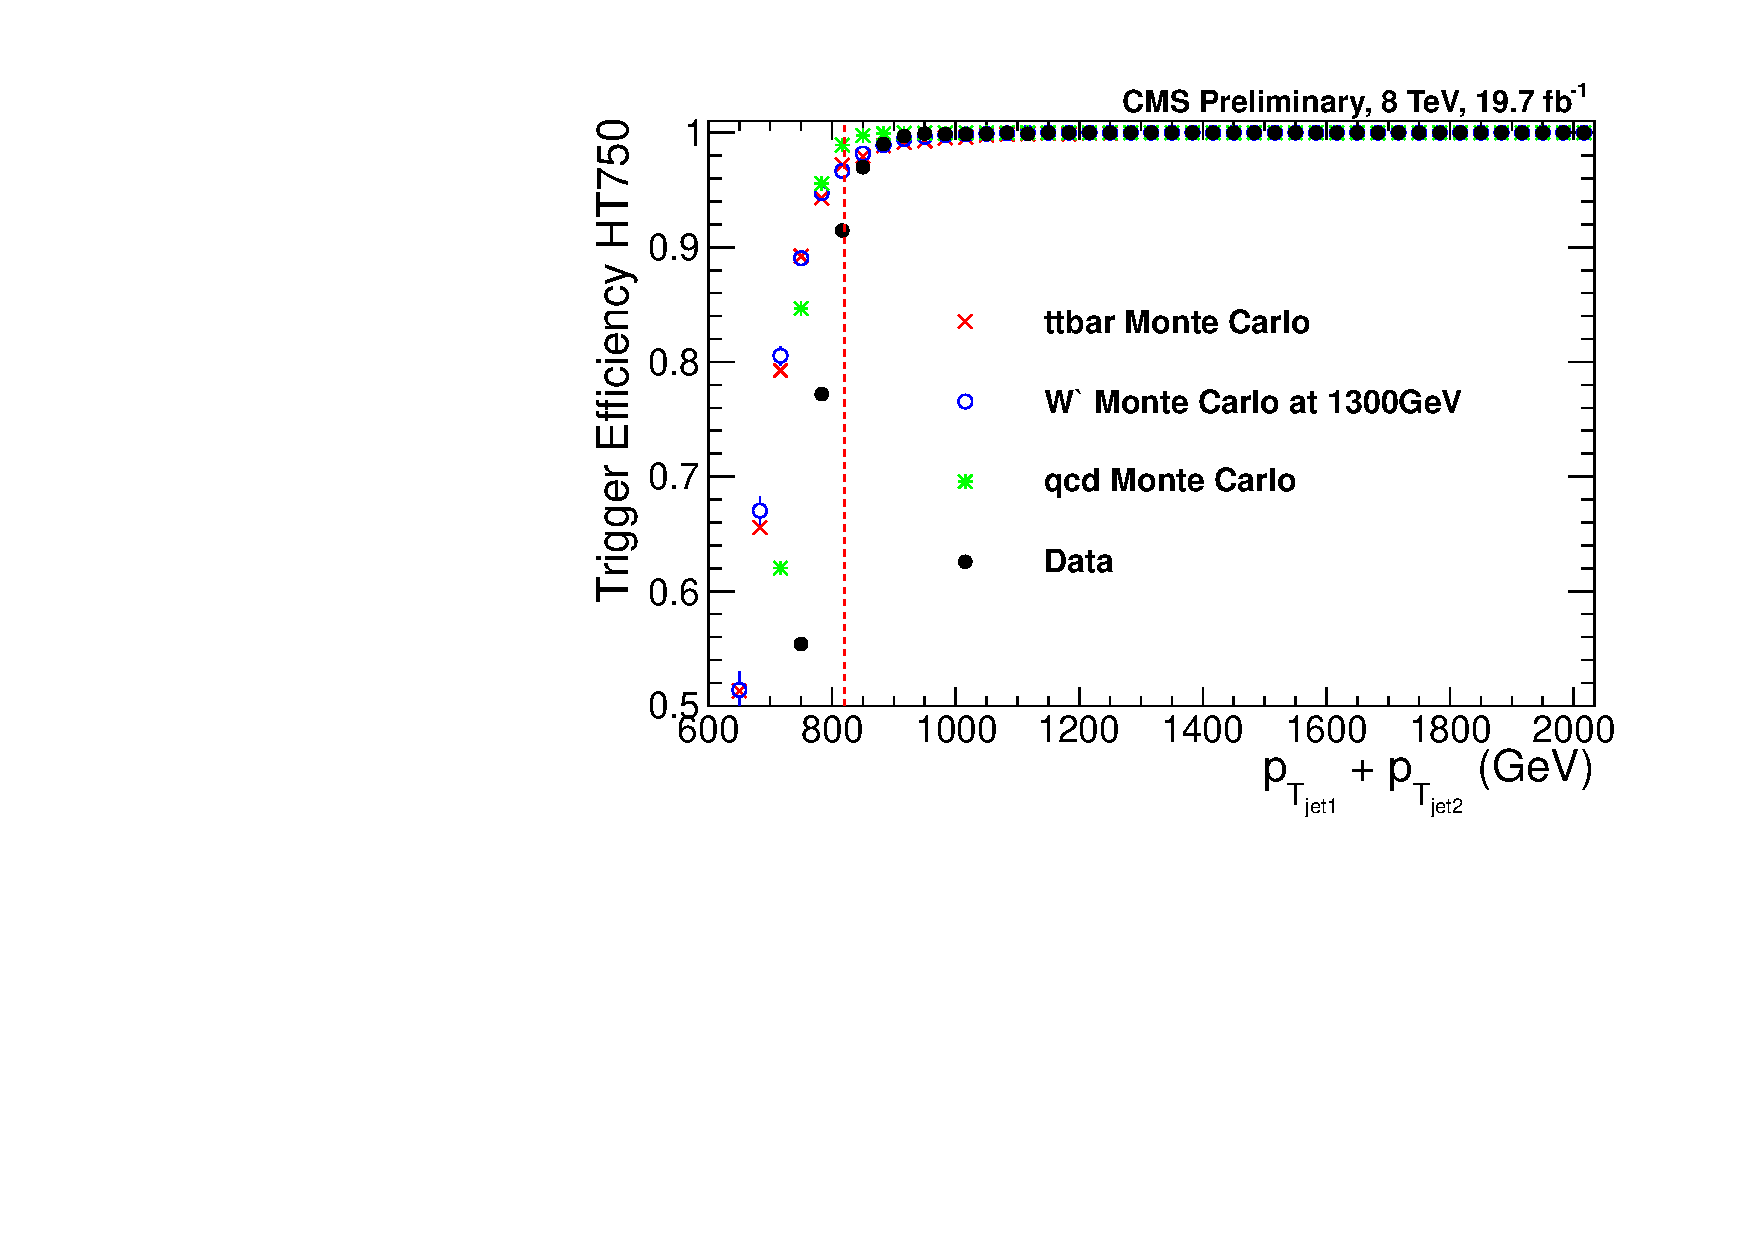
\includegraphics[width=0.9\textwidth]{AN-13-004/figs/Trigger_Comparison_Htdijet.pdf}
\caption{Trigger efficiency of \texttt{HLT\_HT750} measured as a function of the summed $\pt$ of the leading and sub-leading jets.  The red dashed line indicates the minimum for the analysis, 
at which point the trigger is nearly fully efficient.}
\label{figs:Trigger_Comparison_Ht}
\end{figure}

\subsection{Signal Characteristics}
\label{sec:sigchar}
\label{sec:GenBptCut}
The $\wpr$ boson of interest is very massive, and produces highly boosted top quarks.  The decay products of these top quarks become more collimated as the boost 
increases.  When the top decays hadronically, we observe one merged jet over the two distinct jets that would be detected at a lower boost.  This jet has a 
large characteristic radius and a distinct substructure.  This high energy jet merging is investigated in Figure \ref{figs:topmerge}.  Here, the `top candidate' 
is just the leading jet in the event.  It is also required to be hemispherically separated from a MC truth b jet.  This jet is generally a merged W boson at low $\pt$ and a merged top at high $\pt$.
The `W candidate' (used for the bottom plots) is assembled from the pair of generator level non-b quarks that are close to the W mass (within 2.0~$\GeV$).  
The central feature of this analysis is using this jet merging to discriminate signal from background.

\begin{figure}[htcb]
\centering
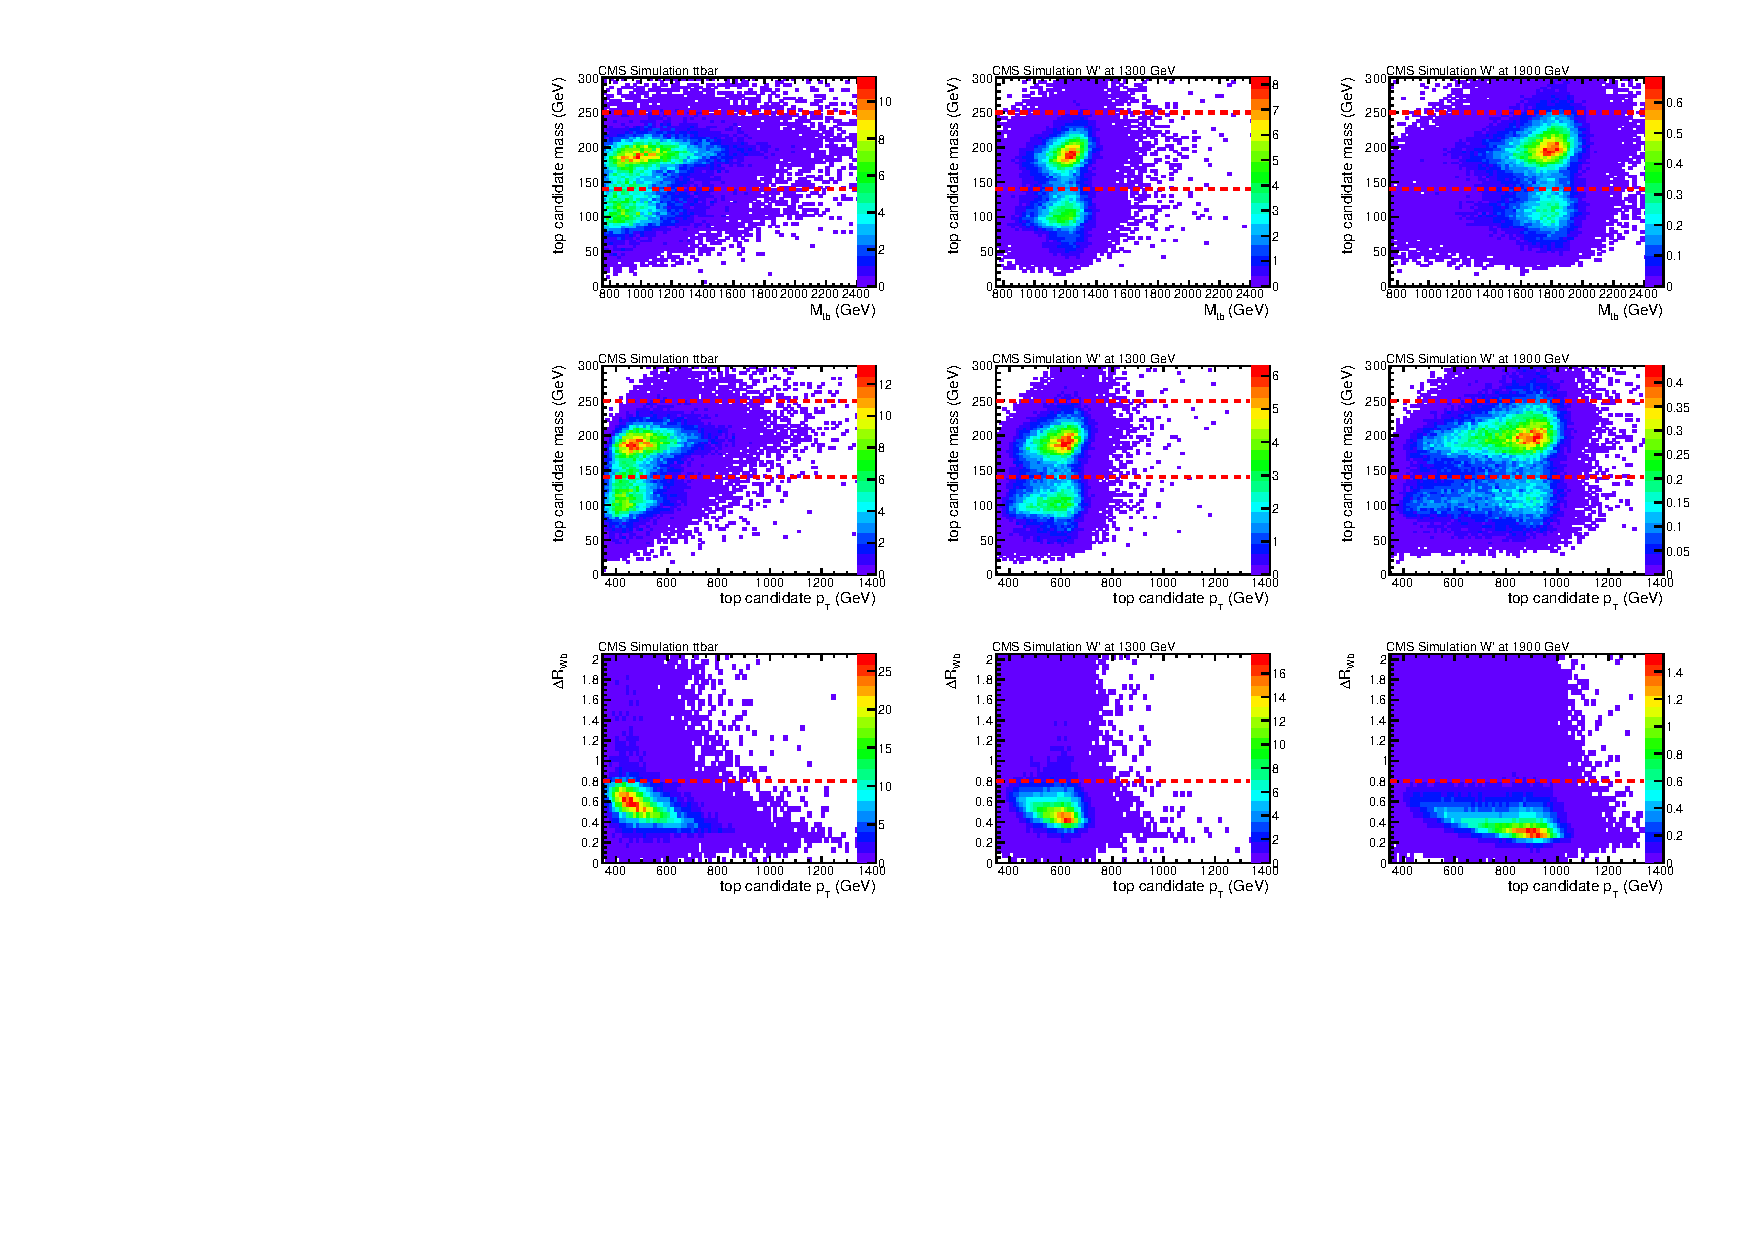
\includegraphics[width=0.9\textwidth]{AN-13-004/figs/topmerge.pdf}
\caption{Investigation of top merging within MC samples of interest.  $\ttbar$ (left) $\wpr_R$ MC at 1300$\GeV$ (middle) $\wpr_R$ MC at 1900$\GeV$ (right).  The red lines on the top and middle plots indicate the top candidate mass cut in the full selection (see Section \ref{sec:toptagging}).  The red line on the bottom plots indicate the characteristic jet radius used to investigate fully merged top jets (see Section \ref{sec:reconstruction}).}
\label{figs:topmerge}
\end{figure}

We place a generator level $\pt$ cut on the b quark from the $\wpr$ decay in the left-handed and mixed-coupling $\wpr$ samples (see Section \ref{sec:signal}).  
To investigate the effect of this pre-selection, we look at the effect of an even tighter cut.  
Figure \ref{figs:genptcut} shows the ratio of generator level b $\pt$ cuts.  
The denominator requires a generation level pt cut of 200 $\GeV$ and the numerator requires a generation level pt cut of 230 $\GeV$.  
This ratio is parameterized in the $\pt$ of the CA8 jet that the generation particle is matched to ($\mathrm{\Delta R  < 0.5}$ is used for matching).
The turn on of this tighter cut is well below the analysis level cut of 370$~\GeV$.  Thus, the effect of the generation level b $\pt$ cut 
on selections requiring the analysis level $\pt$ cut is negligible.  

\begin{figure}[Htcb]
\centering
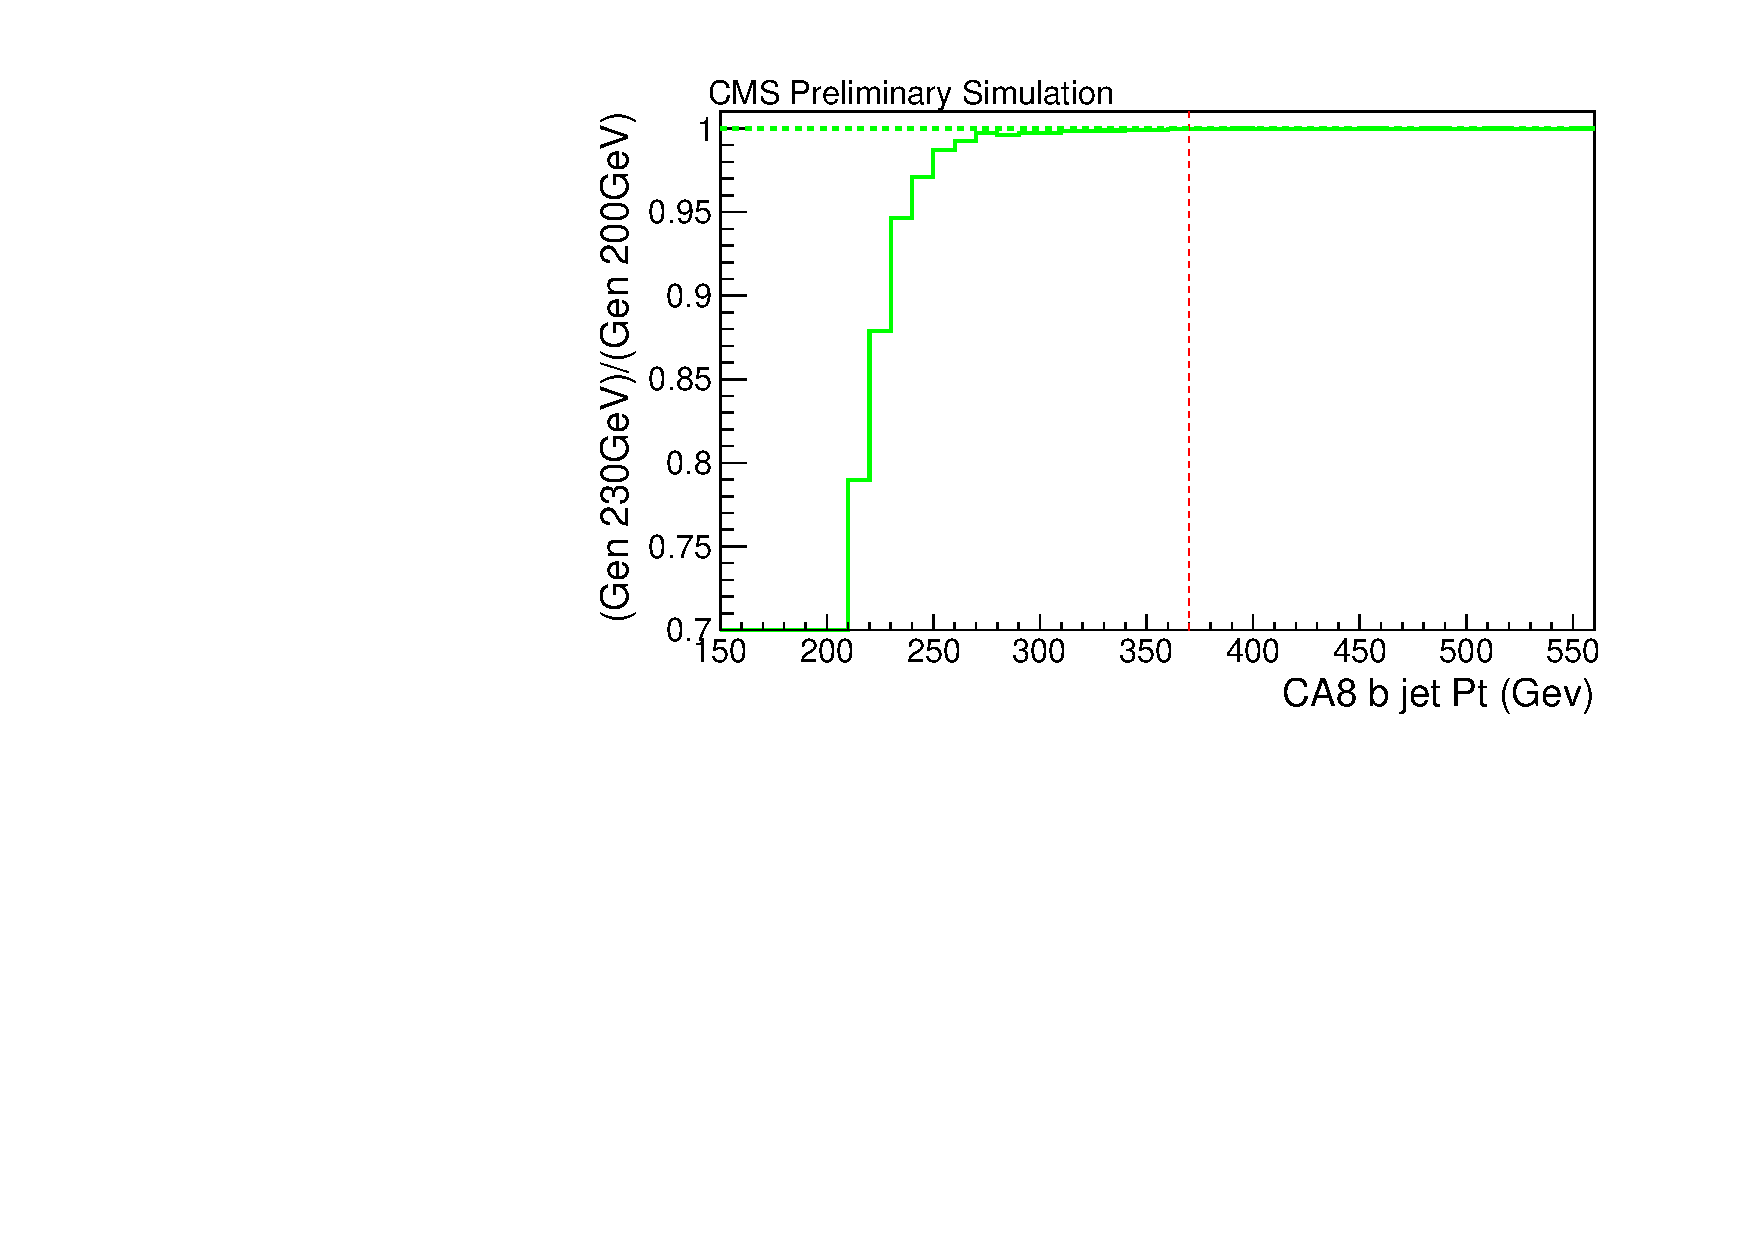
\includegraphics[width=1.0\textwidth]{AN-13-004/figs/bjetptcut.pdf}
\caption{Ratio of CA8 $\pt$ using the generation level b pt cut of 230$~\GeV$ and 200$~\GeV$.  The red line is the analysis level $\pt$ cut of 370$~\GeV$.  The sample used for this study is $\wpr_{LR}$ at 1300$~\GeV$}
\label{figs:genptcut}
\end{figure}



\subsection{Jet Reconstruction}
\label{sec:reconstruction}
All data are reconstructed using CMSSW 5.3.x, and we use jet energy corrections from \verb!FT_53_V21_AN5! \cite{CMS-DP-2013-033}.  The Particle Flow reconstruction algorithm is used 
to reconstruct all data and MC samples used for the analysis.  This algorithm uses information from all sub-detectors 
to categorize particles as muons, electrons, photons as well as charged and 
neutral hadrons.  Charged hadrons identified as pileup are removed from the inputs to the jet clustering algorithms by Charged Hadron Subtraction (CHS).
Pileup vertices are identified as vertices that have a lower $\pt$ than the primary vertex.  Isolated charged leptons are removed,
and neutral pileup components are removed with a residual area-based method.  For more detail, see \cite{7tevZprime}.  
The PF candidates are then used to create 'Particle Flow jets' as follows.  Jet clustering is performed 
with a sequential recombination algorithm which compiles jets by merging the minimum of 
$\mathrm{d_{ij} = min(k_{Ti}^{2m},k_{Tj}^{2m})\Delta _{ij}/R}$ where $\mathrm{\Delta _{ij} = \sqrt{(y_i-y_j)^2 + (\phi _i-\phi _j)^2}}$.
  We use the Cambridge-Aachen (CA) \cite{CAcambridge,CAaachen} algorithm implemented by FastJet 3 \cite{fastjet1,fastjet2}, 
which assigns a value of $\mathrm{m = 0}$, and thus is not weighted by $\pt$.  An R value 
of 0.8 is used for the analysis.  The CA algorithm has been shown to be more efficient than the 
the $\mathrm{k_{T}}$ and the anti-$\mathrm{k_{T}}$ algorithms for finding hard subjets \cite{catop_cms}.

%The corrections for the CA $R=0.8$ jets are derived from the
%anti-$k_{\mathrm T}$ $R=0.7$ jet algorithm. 
We use anti-$\mathrm{k_{T}}$ jet energy corrections for all jets in the analysis. 
The jet energy corrections derived are adequate for the CA $\mathrm{R=0.8}$ jet algorithm for the jet momenta
considered here as can be seen from 7~$\TeV$ studies in simulation comparing AK5 and CA8 jets \cite{7tevZprime}.  
We use the 2012 prescription for jet energy corrections\cite{JEC2012}.  We apply AK7 
Particle Flow with charged hadron subtraction 
(AK7PFchs) jet energy corrections for all data and MC samples.

\subsection{Event Pre-selection}
\label{sec:pre-selection}
The following pre-selection is applied:

\begin{itemize}
\item The event must have a good primary vertex as computed by a deterministic annealing filter (DAF)
($\vert z_\text{Primary Vertex}\vert < 24$ cm, $N_\text{DOF} > 6$).
\item Two jets with $|y| < 2.4$
\item Only two jets with $\pt > 150~\GeV$
\item Leading Jet $\pt > 450~\GeV$ \& Sub-leading Jet $\pt > 370~\GeV$
\item Loose Particle Flow jet identification \cite{jetid} is applied
\item Leading and sub-leading jet are separated by $|\Delta y| < 1.6$.  This cut is described in Section \ref{sec:deltarapidity}.
\item Beam background events are removed using the following requirements:
        \begin{itemize}
        \item In events with at least 10 tracks, a minimum of 25\% of
          these tracks must be high purity tracks.
        \end{itemize}
\end{itemize}


The requirement that there are only two jets with $\pt > 150~\GeV$ is useful for vetoing ``three-prong'' trijet events, which could impact the kinematics of the top-W candidate invariant mass 
distribution and bias the background estimate. 

\subsection{$\ttbar$ $\pt$ Re-weighting}
\label{sec:ttptrw}
In order to correct for known differences in the top $\pt$ spectrum between data and $\ttbar$ MC, we re-weight MC using the Generator level $\pt$ of the top and anti-top with the recommended prescription.  
With $\mathrm{p_{T_{t}}}$ and $\mathrm{p_{T_{\overline{t}}}}$ being the generator $\pt$ of the top and anti-top respectively, the scale factor applied to each event in the $\ttbar$ MC expectation is:
\begin{eqnarray}
\mathrm{SF =\sqrt{e^{0.156-.00137p_{T_{t}}} \times e^{0.156-.00137p_{T_{\overline{t}}}}}}
\end{eqnarray}
Although this procedure was not designed for the kinematic range in our analysis, 
we prefer to use the prescription as it is more consistent with our measurement of the $\ttbar$ normalization (see Section \ref{sec:ttbarsideband}).


\subsection{Pileup Correction}
\label{sec:pileup}
We re-weight our MC samples to account for differences due to pileup using the recommended procedure.  
To create a scale factor for number of primary vertices, we use MC truth to extract the number of pileup interactions.  
Then we compare this to the mean number of interactions per crossing from data.  
This is extracted using the pileup distribution from the rereco datasets listed in table \ref{table:datasets}.  
For this calculation we use the suggested minbias cross-section of 69.4 mb.  The scale factor is then 
the data distribution divided by the distribution in MC and is applied to the signal and $\ttbar$ MC samples to improve 
data to MC agreement.
Figure \ref{figs:npvweight} shows the distribution of reconstructed primary vertices in Data, $\ttbar$,
and signal MC before and after the re-weighting has been applied. The pileup correction has very little effect on the eventual $\mathrm{M_{tb}}$ full selection, as 
seen in Figure \ref{figs:pileup3}, for $\wpr_R$ signal MC at the 1900$~\GeV$ mass point. Similarly, there is little effect 
$\ttbar$ MC as can be seen in Figure \ref{figs:pileup3ttbar}.  
A study has been conducted to investigate the effect of the suggested systematic uncertainty of 5\% on the  as can be seen in Section \ref{sec:systematics}.  
Figure \ref{figs:PUplots} shows the number of primary vertices in data and signal MC with respect to discrimination variables used to separate signal from background.

\begin{figure}[Htcb]
\begin{center}
\subfigure{\label{figs:sub_data}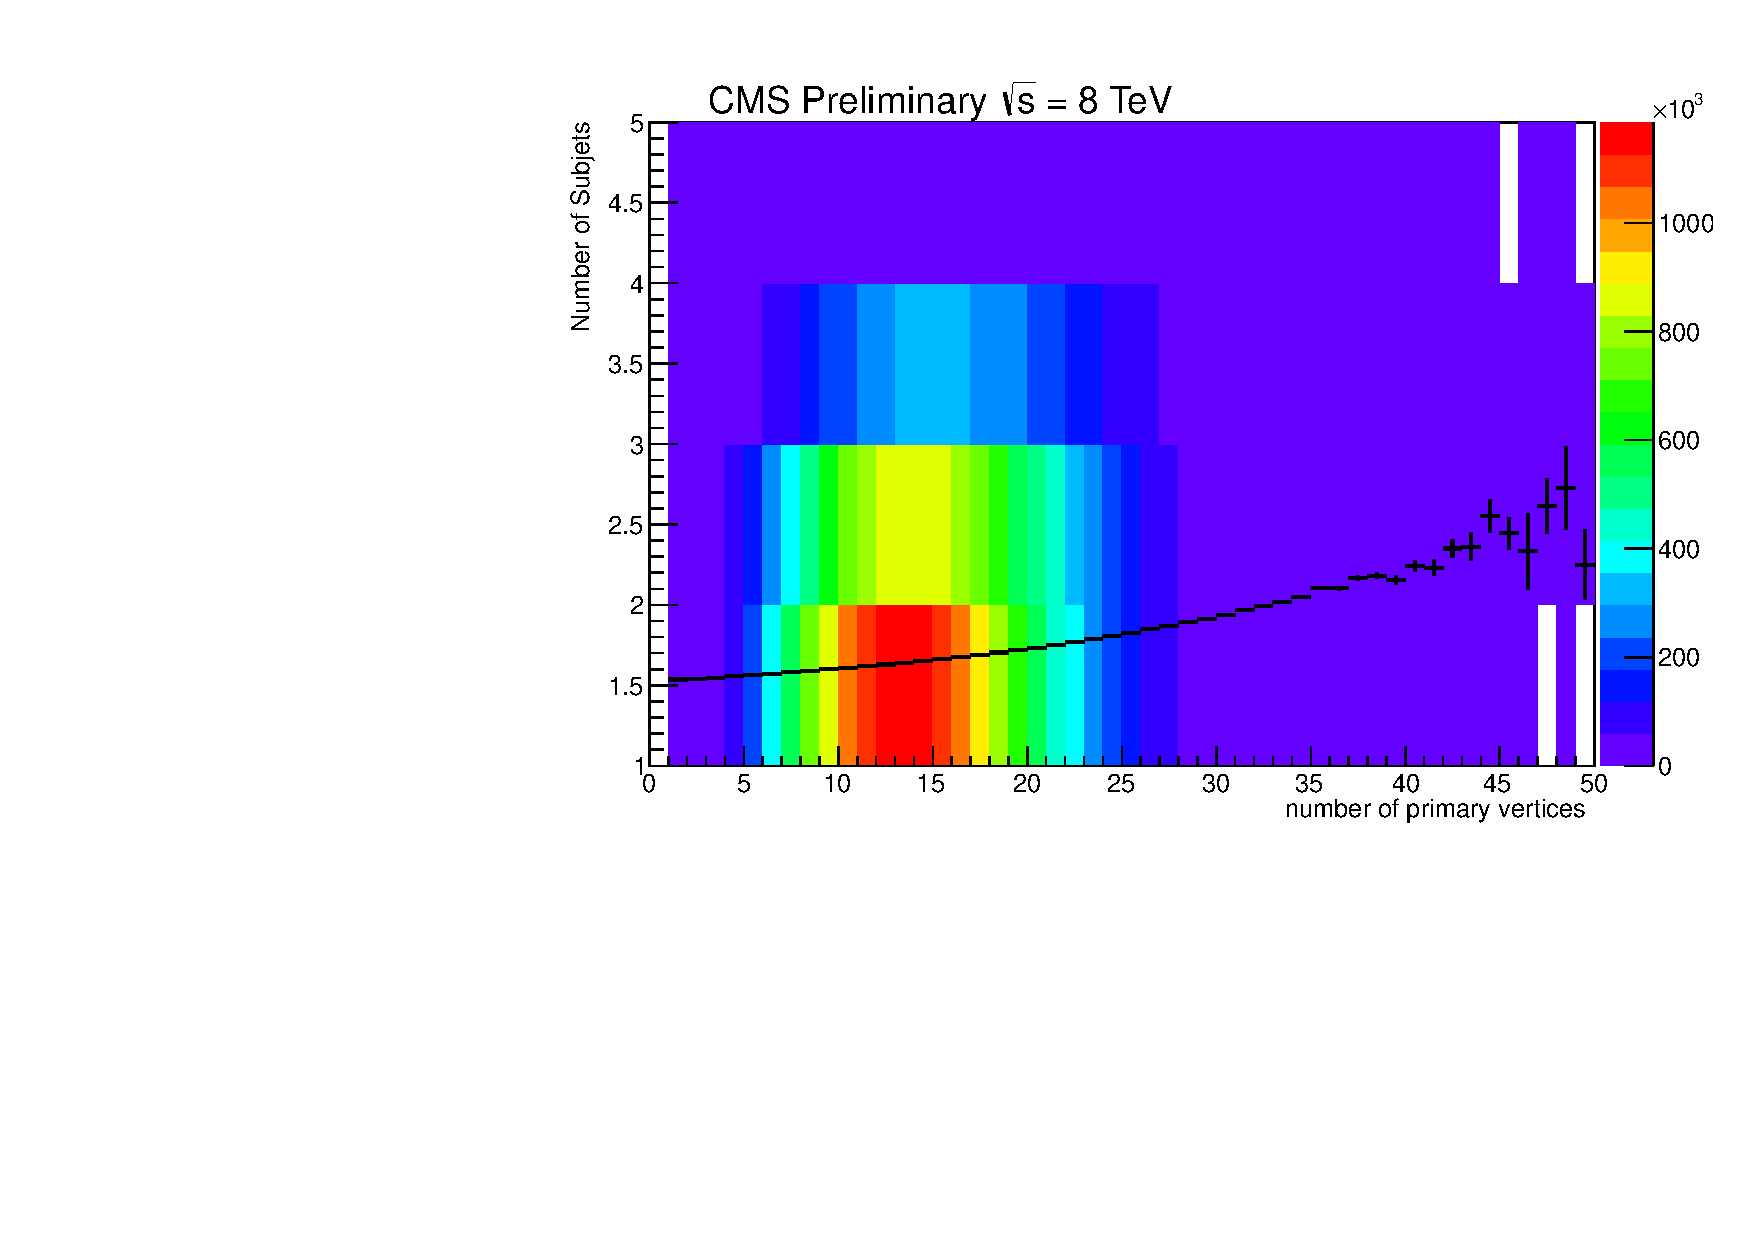
\includegraphics[width=0.4\textwidth]{AN-13-004/figs/sub_data.pdf}}
\subfigure{\label{figs:sub_signal}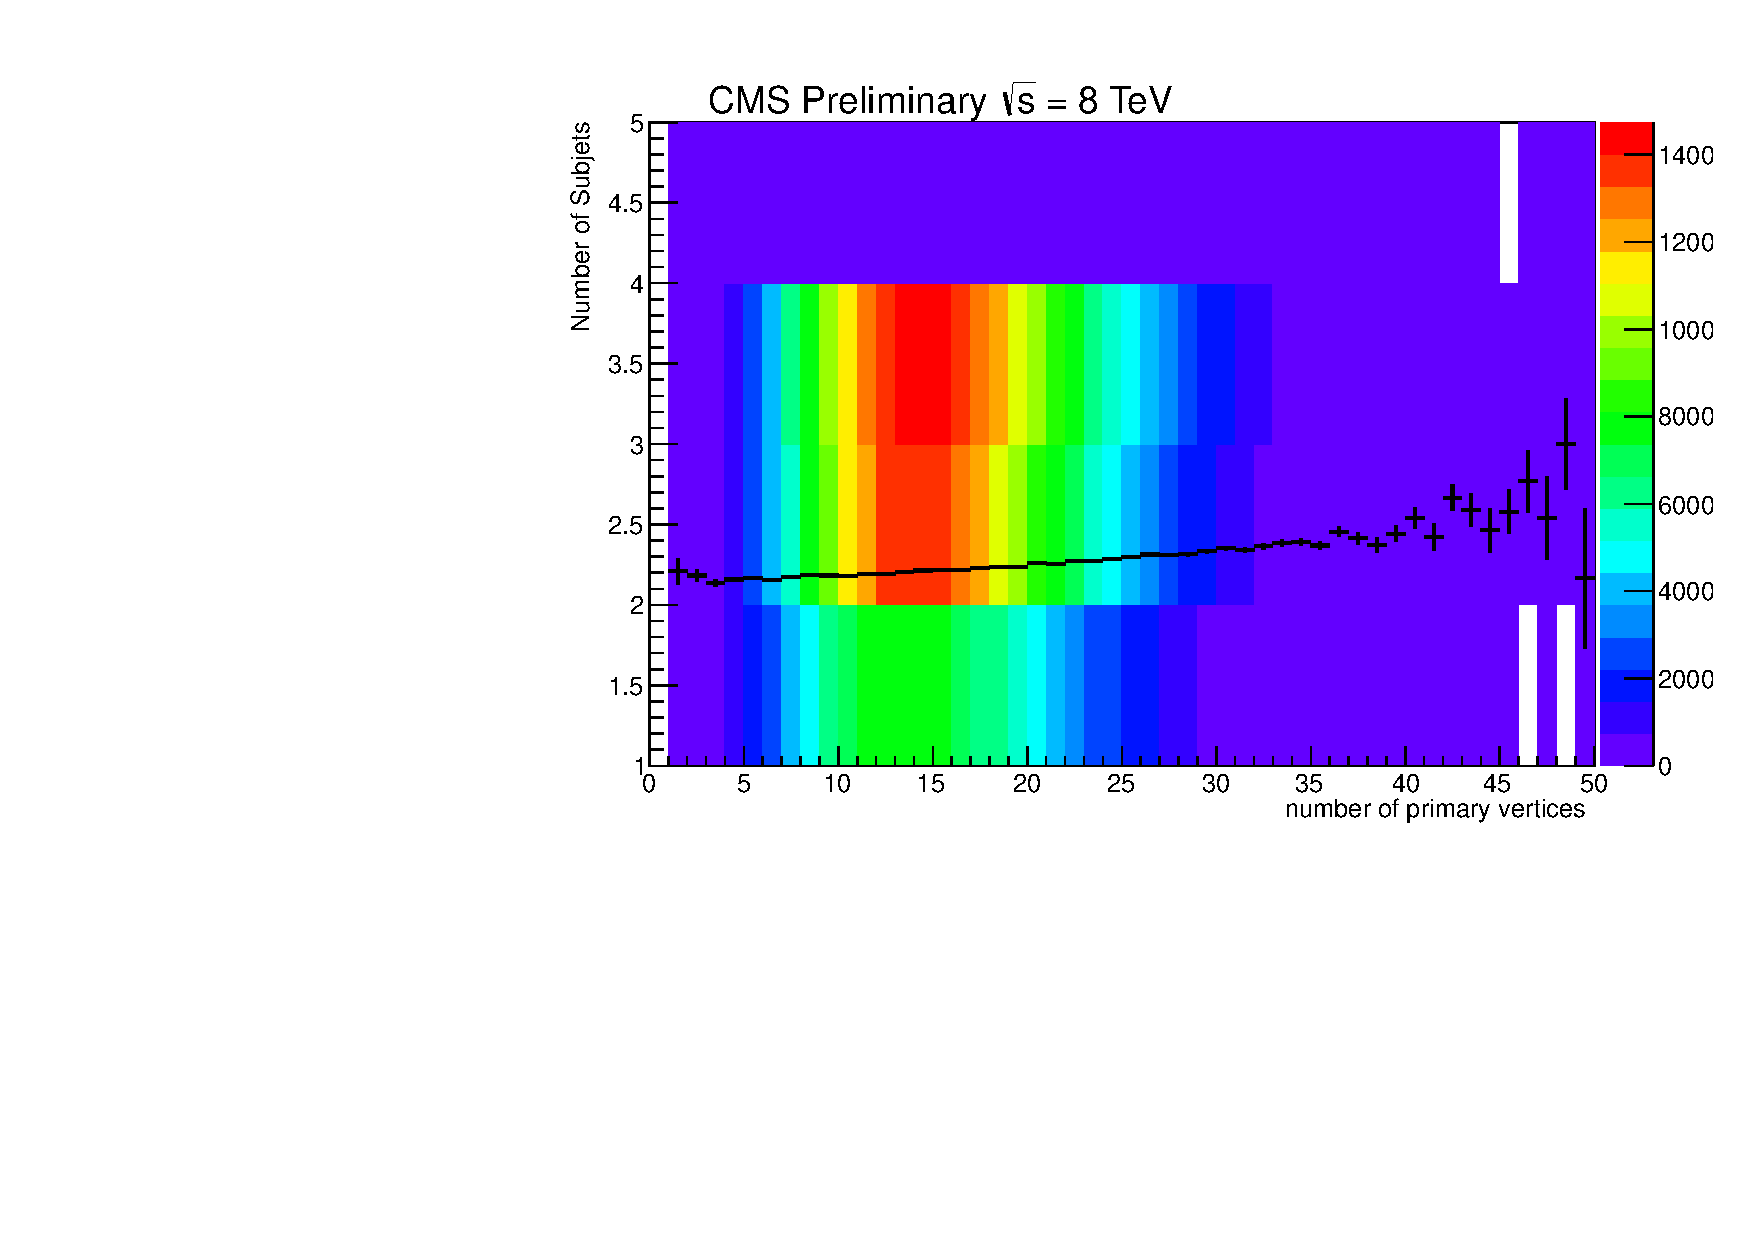
\includegraphics[width=0.4\textwidth]{AN-13-004/figs/sub_signal.pdf}}\\
\subfigure{\label{figs:min_data}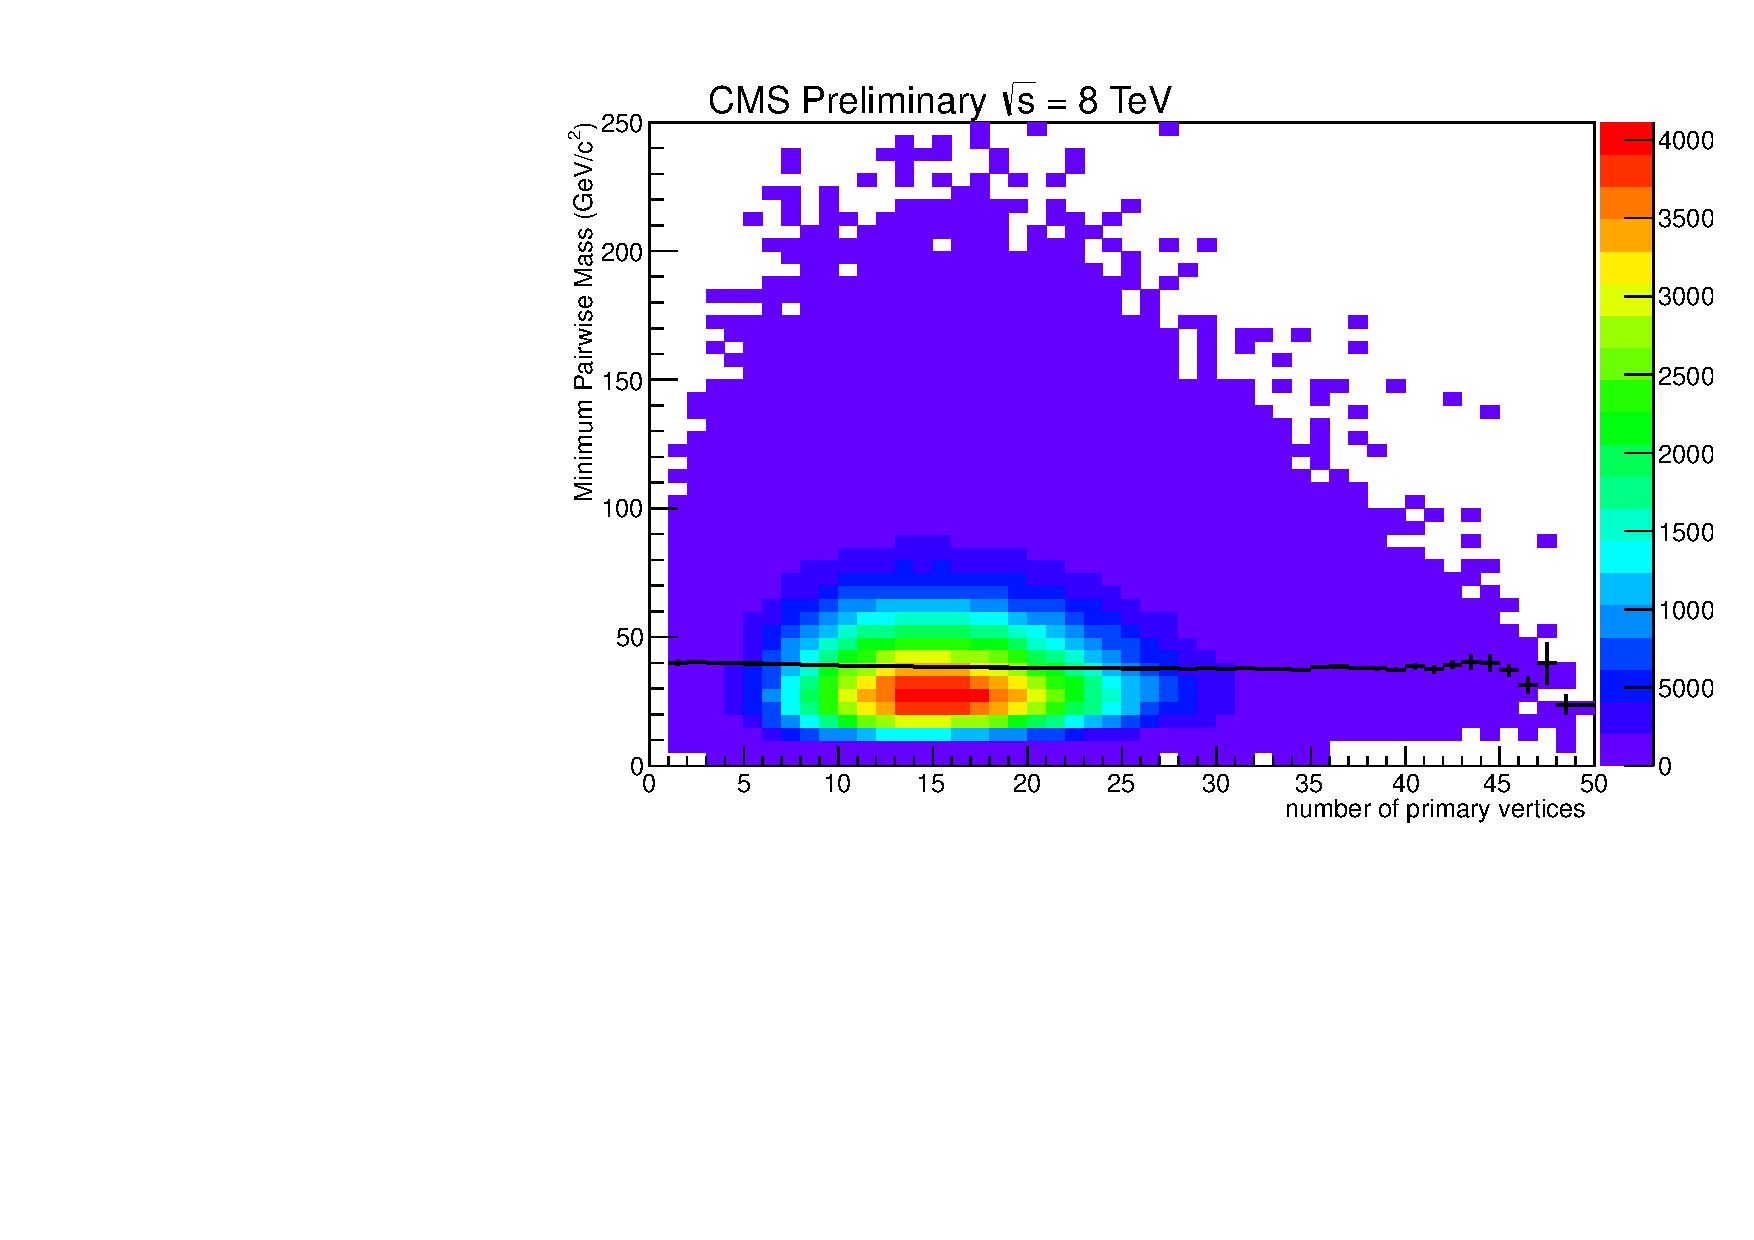
\includegraphics[width=0.4\textwidth]{AN-13-004/figs/min_data.pdf}}
\subfigure{\label{figs:min_signal}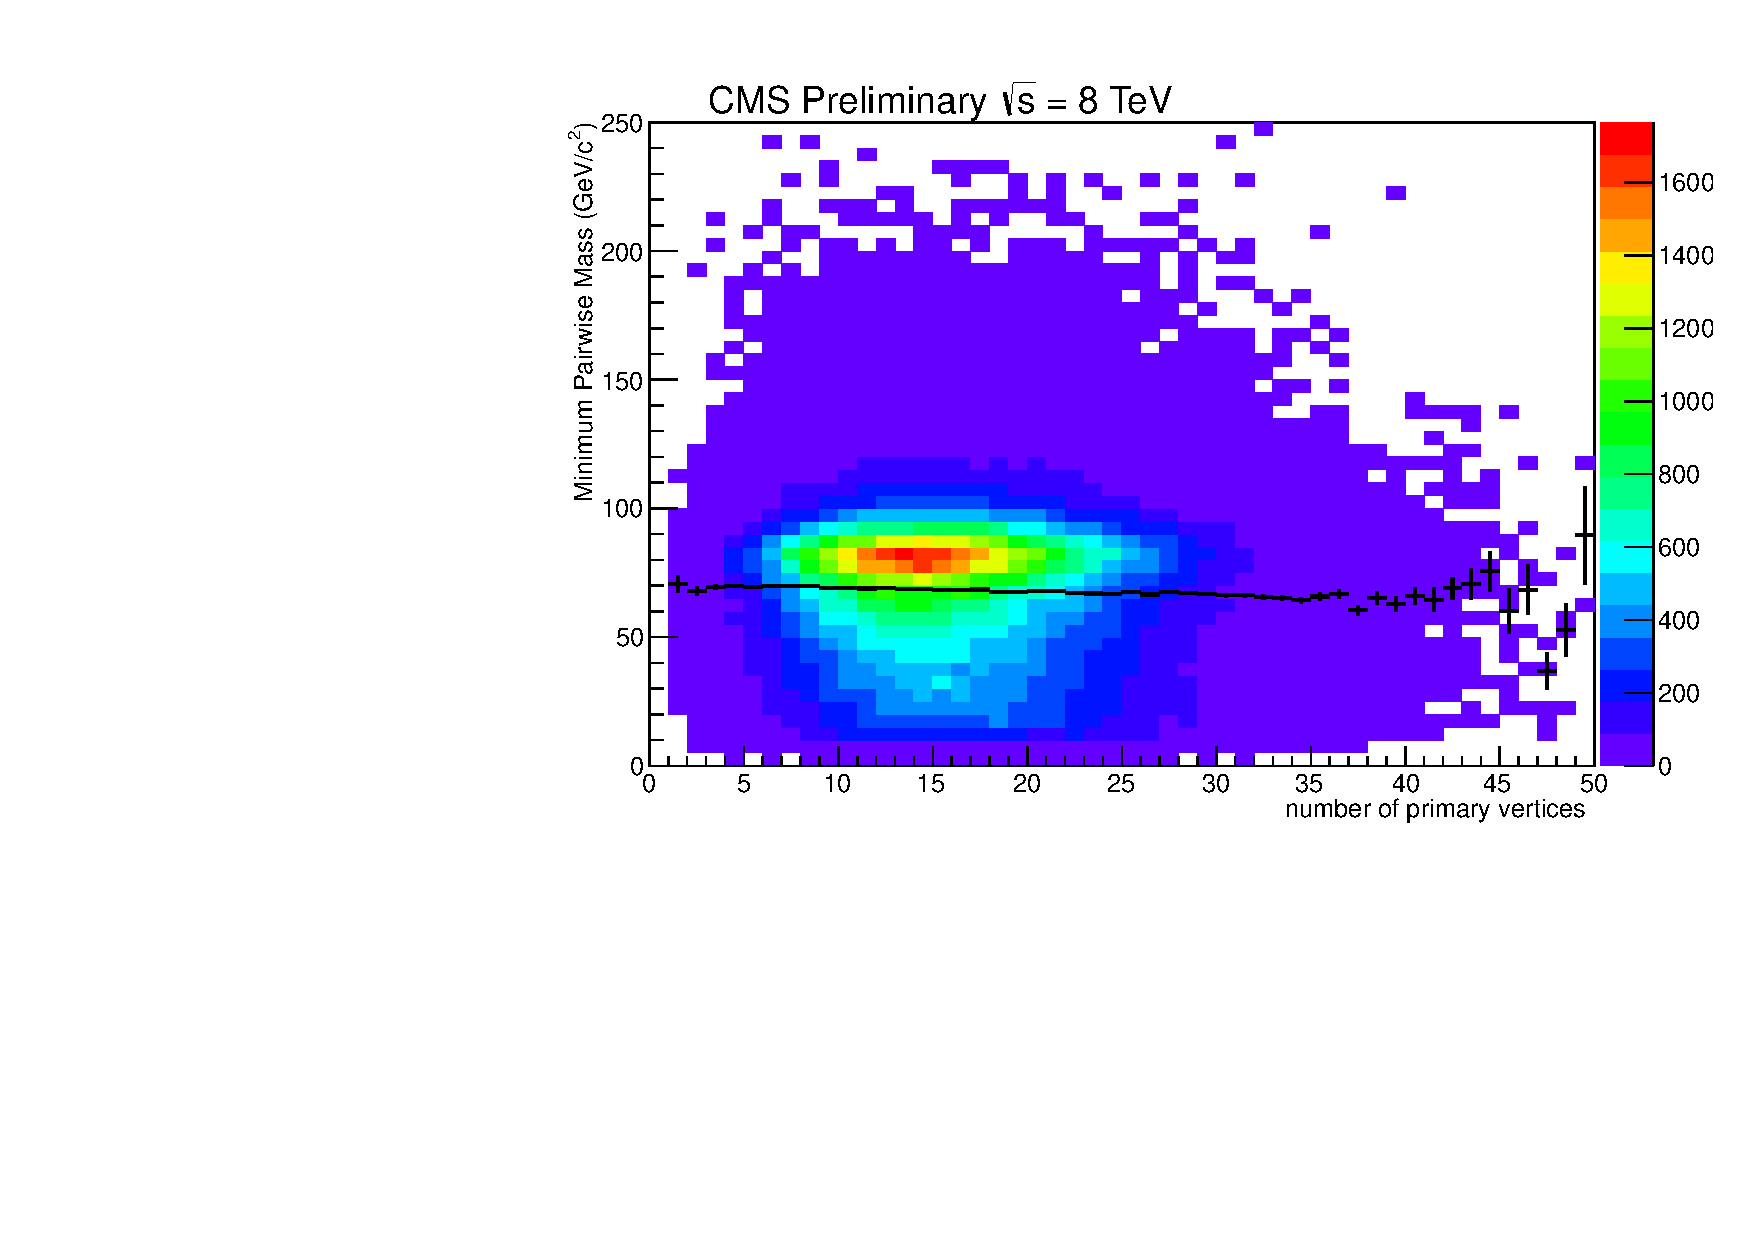
\includegraphics[width=0.4\textwidth]{AN-13-004/figs/min_signal.pdf}}\\
\subfigure{\label{figs:top_data}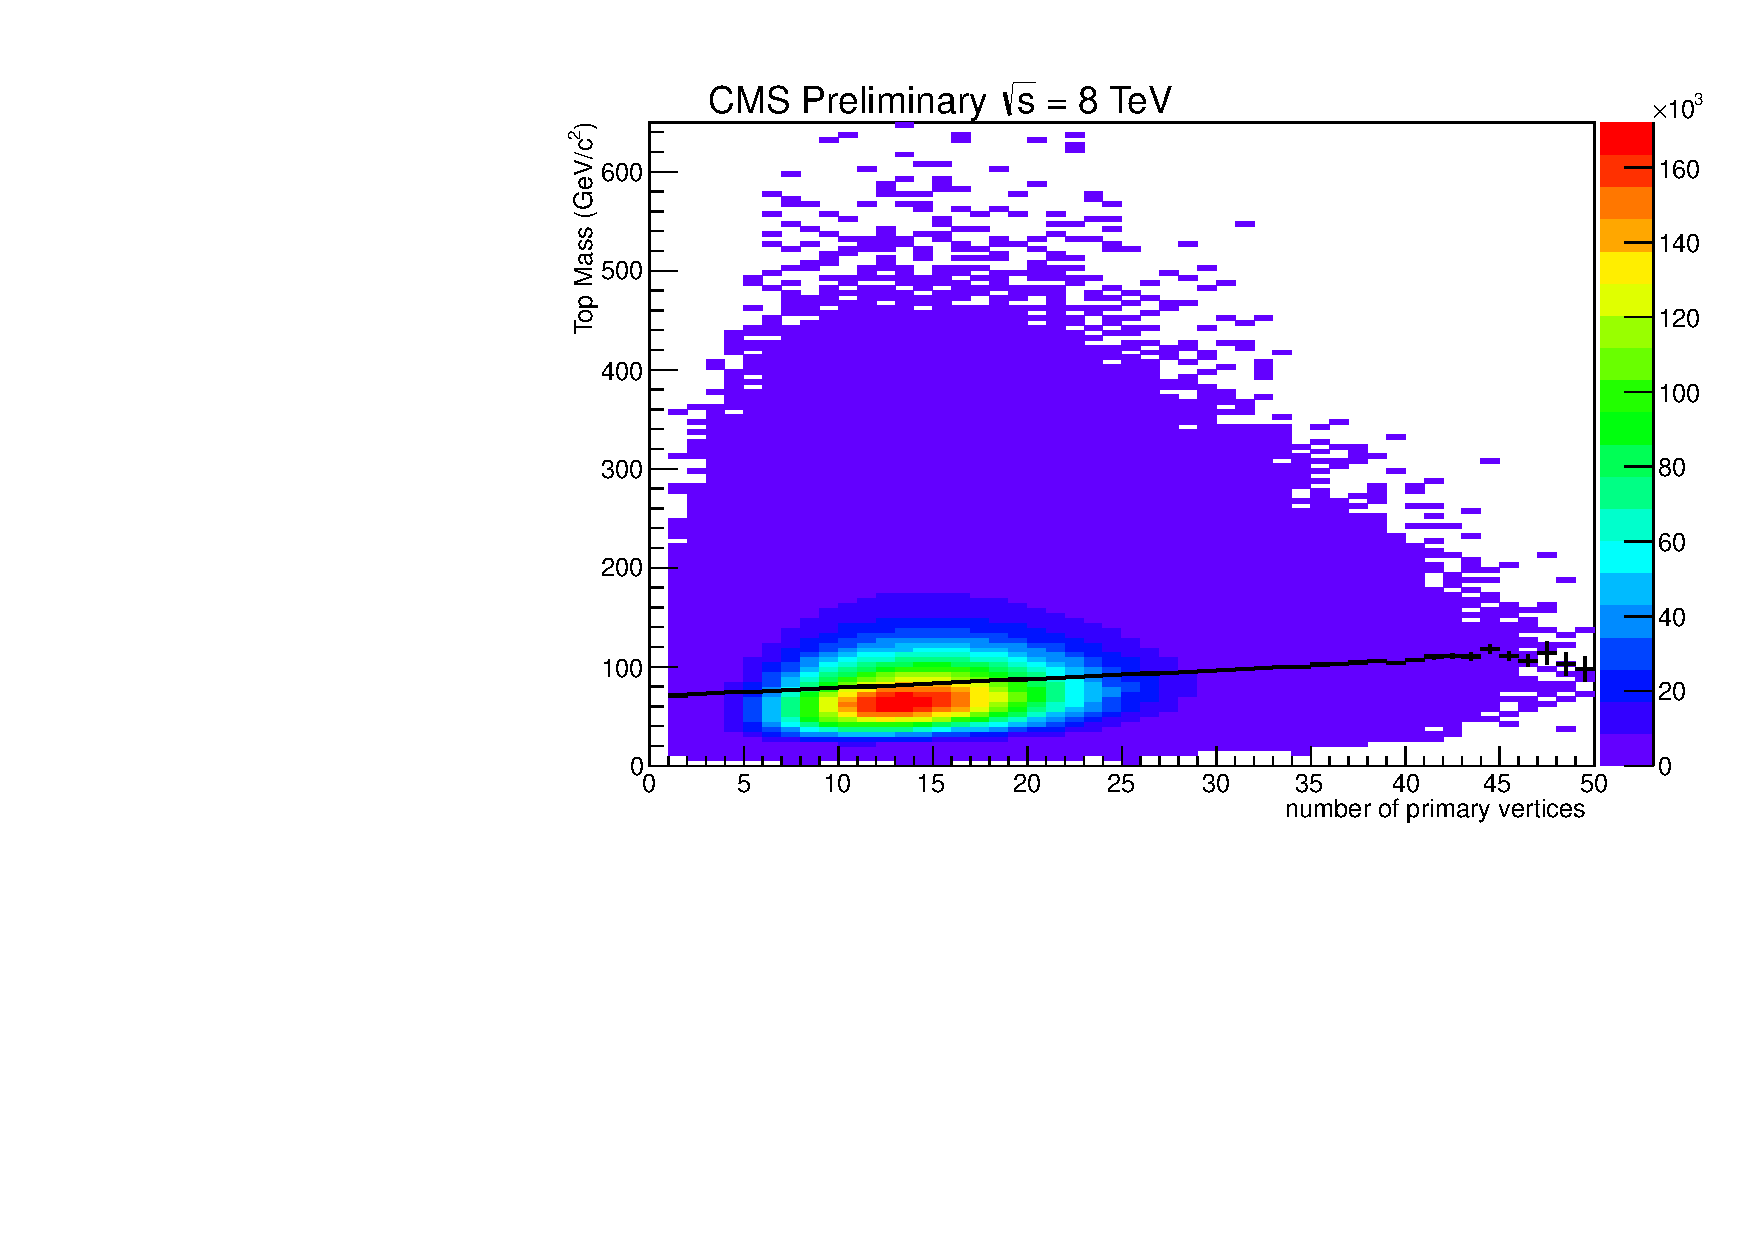
\includegraphics[width=0.4\textwidth]{AN-13-004/figs/top_data.pdf}}
\subfigure{\label{figs:top_signal}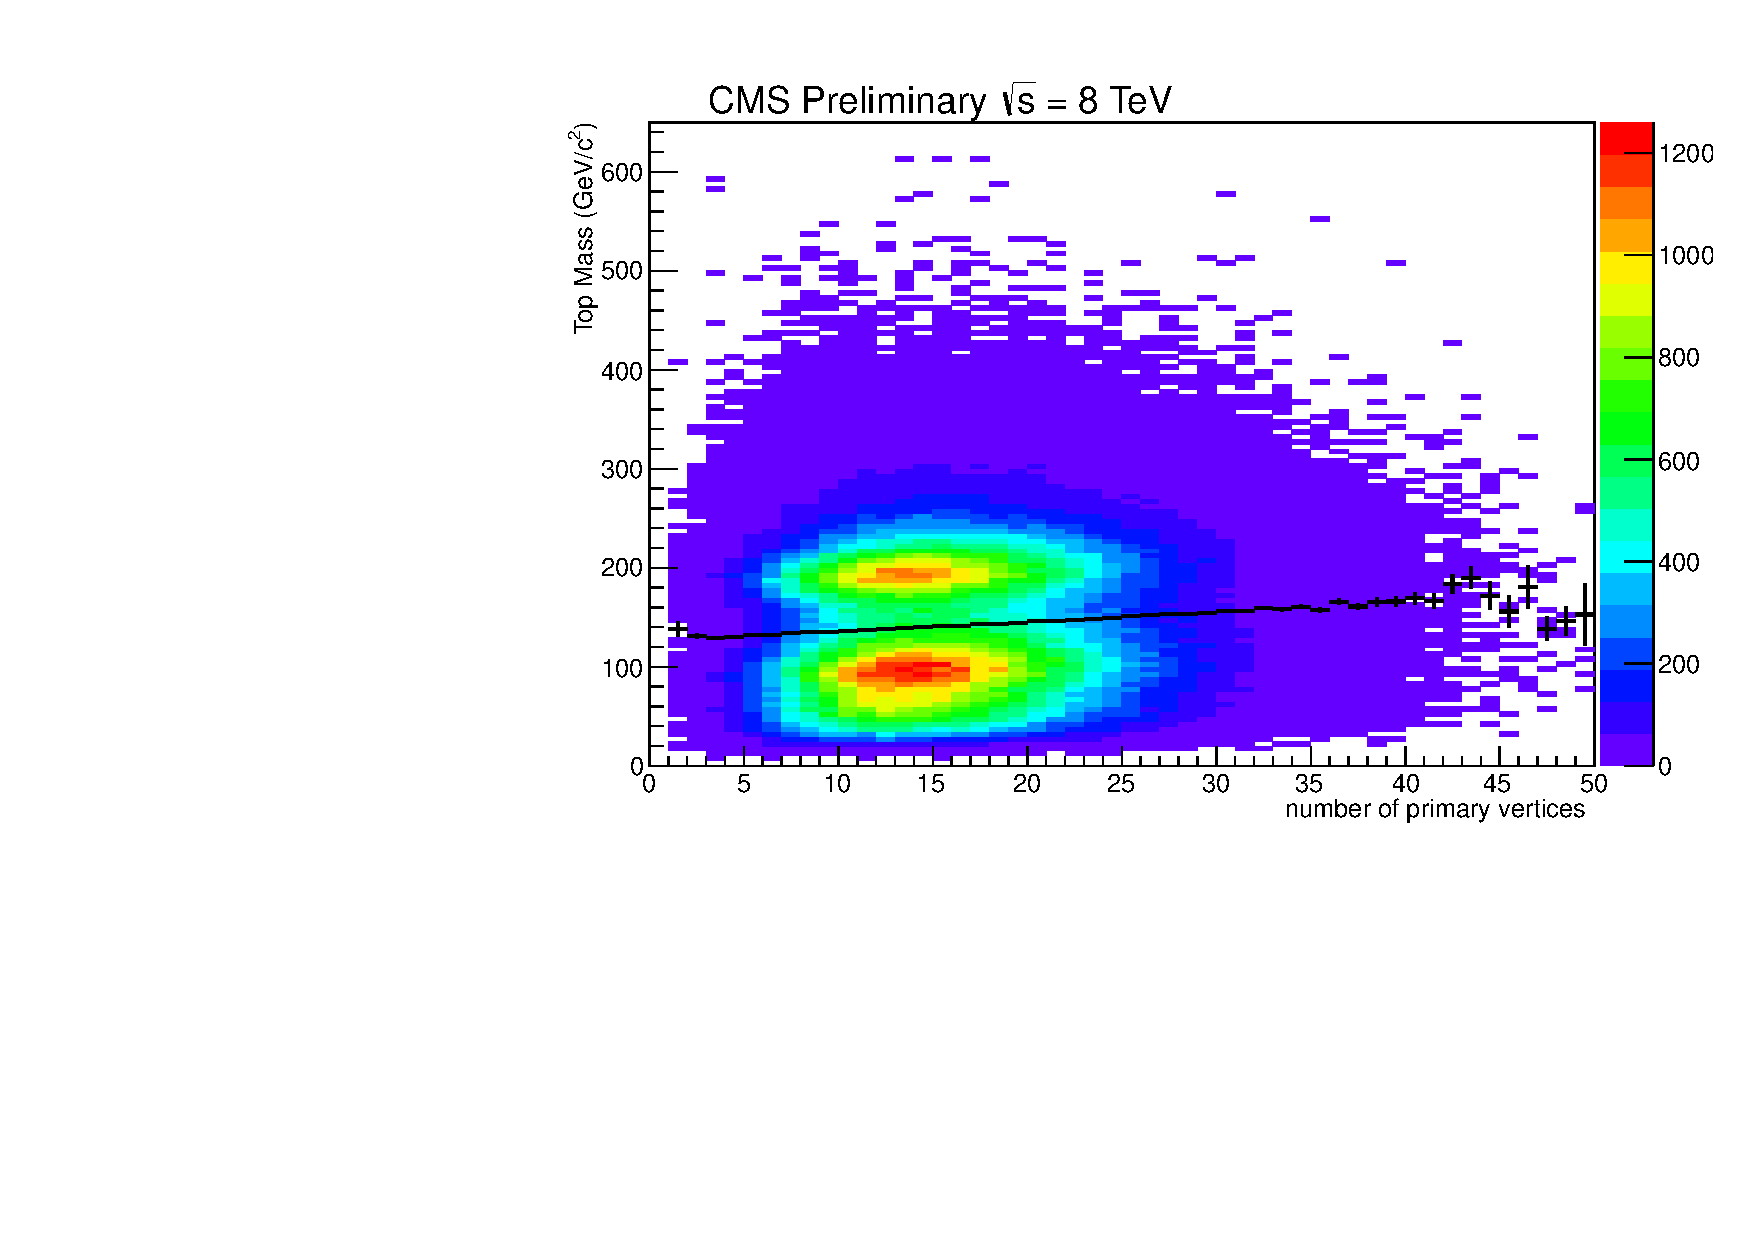
\includegraphics[width=0.4\textwidth]{AN-13-004/figs/top_signal.pdf}}\\
\subfigure{\label{figs:tag_data}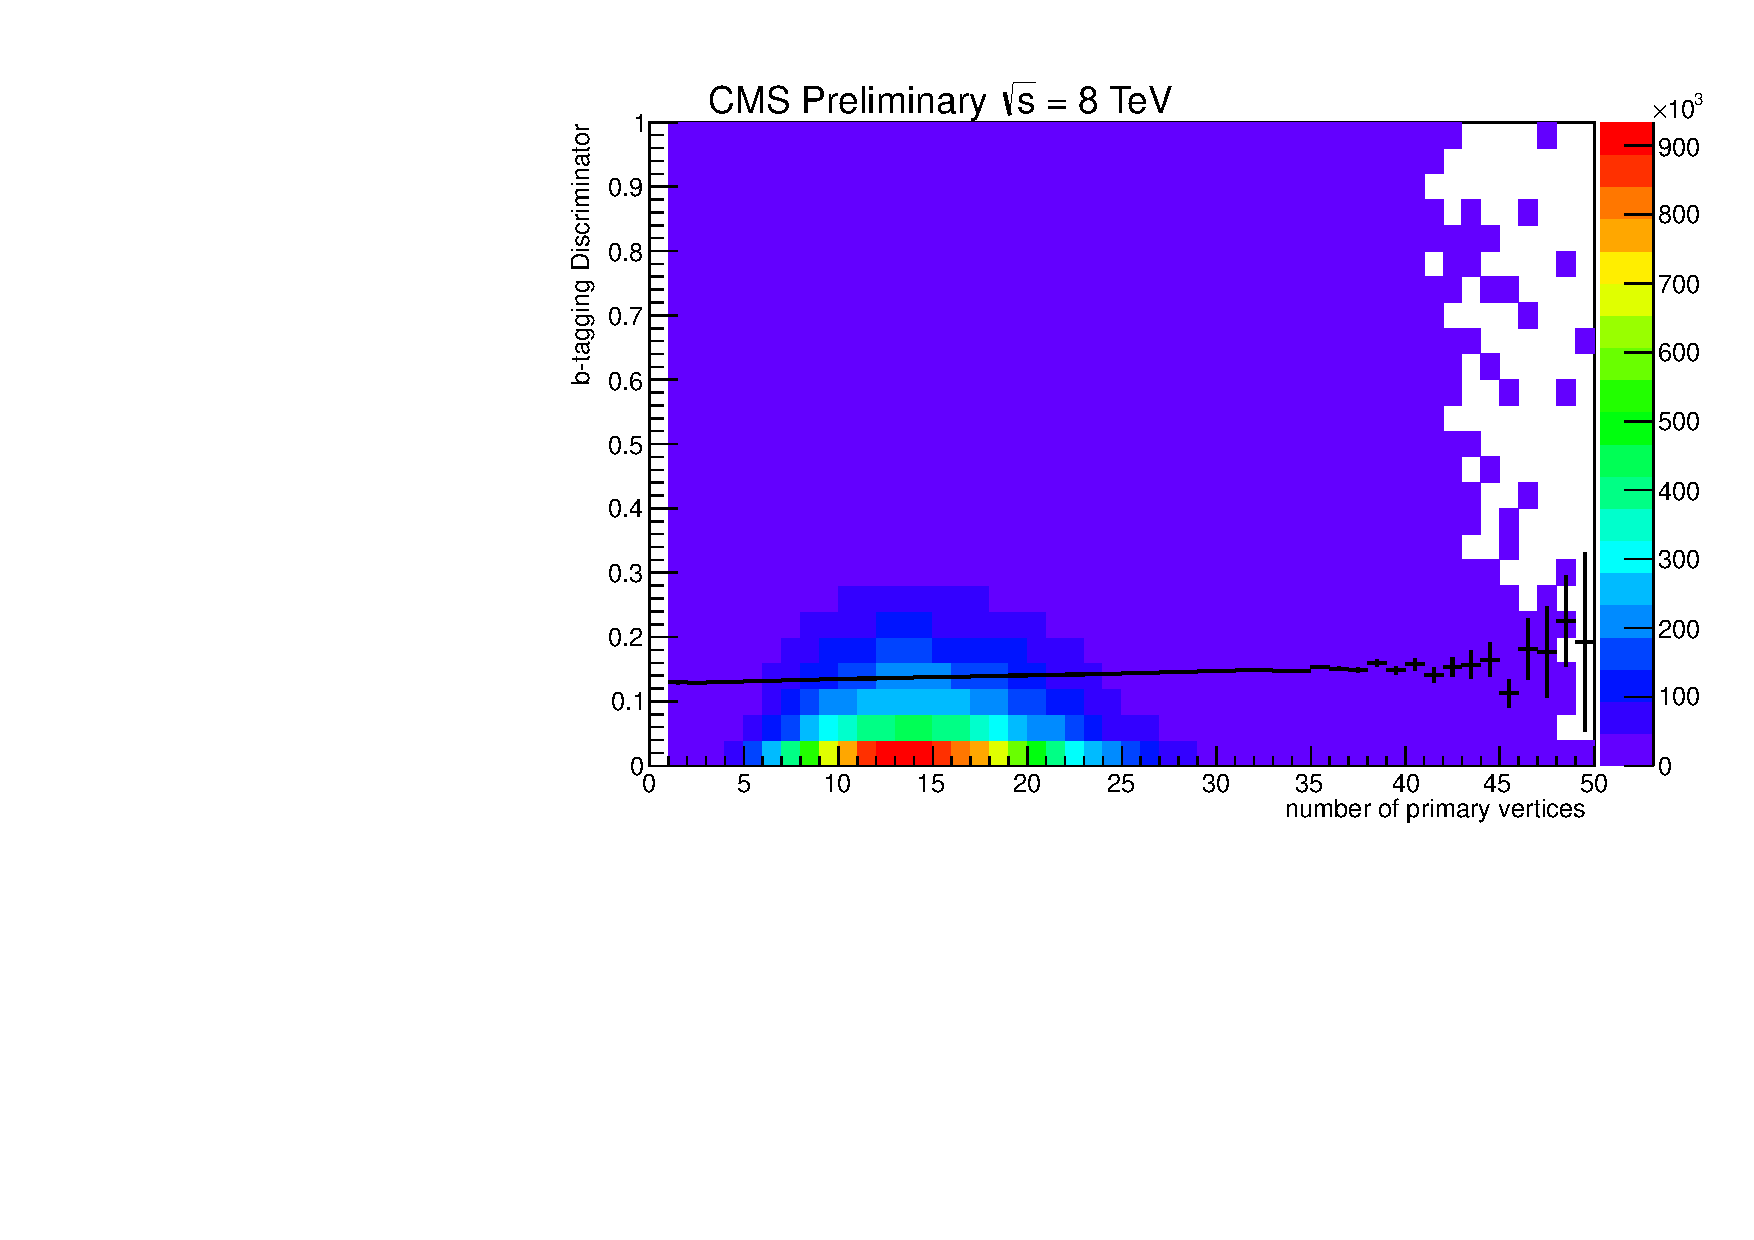
\includegraphics[width=0.4\textwidth]{AN-13-004/figs/tag_data.pdf}}
\subfigure{\label{figs:tag_signal}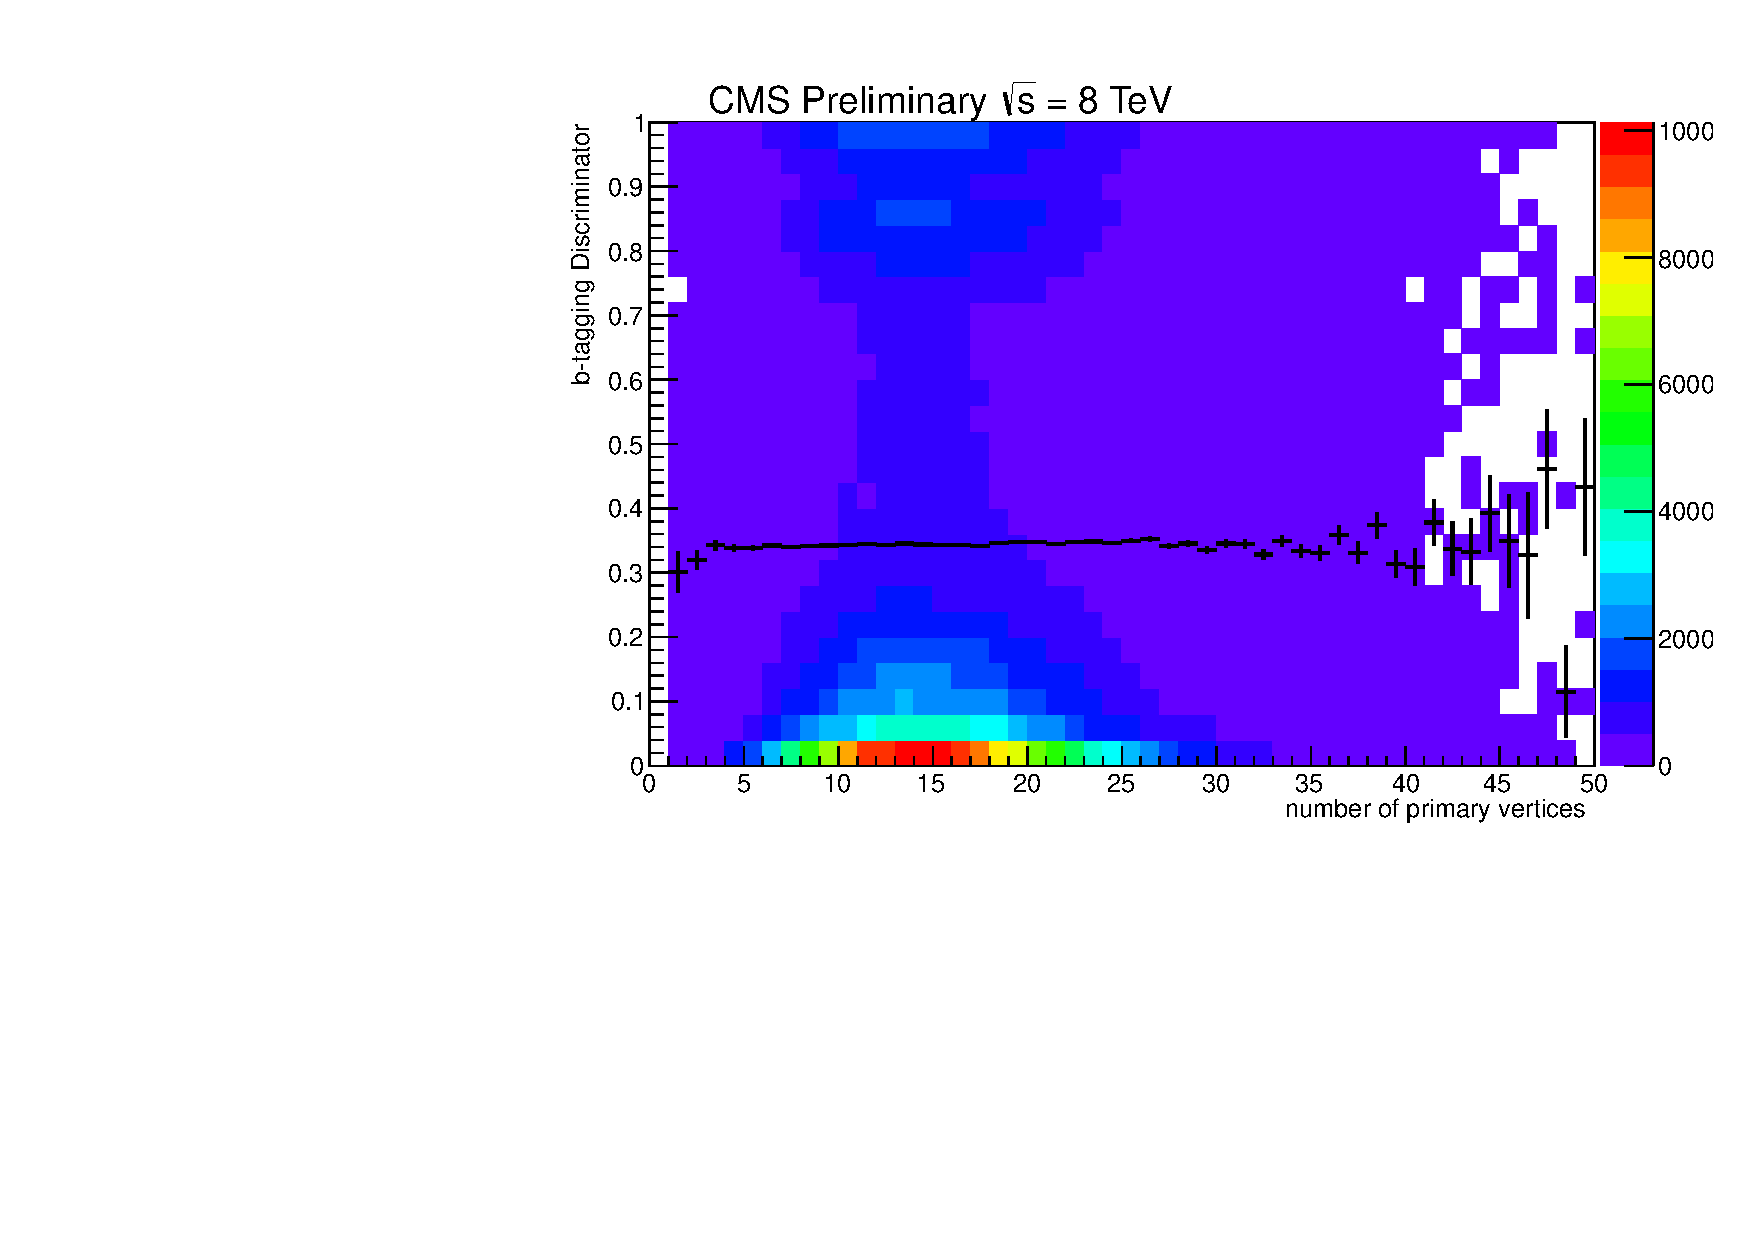
\includegraphics[width=0.4\textwidth]{AN-13-004/figs/tag_signal.pdf}}
\caption{
Number of primary vertices in data and signal MC vs
(a) Number of Subjets  
(b) Minimum Pairwise Mass
(c) Top Mass
(c) CSV b discriminant 
}
\label{figs:PUplots}
\end{center}
\end{figure}


\begin{figure}
\begin{center}
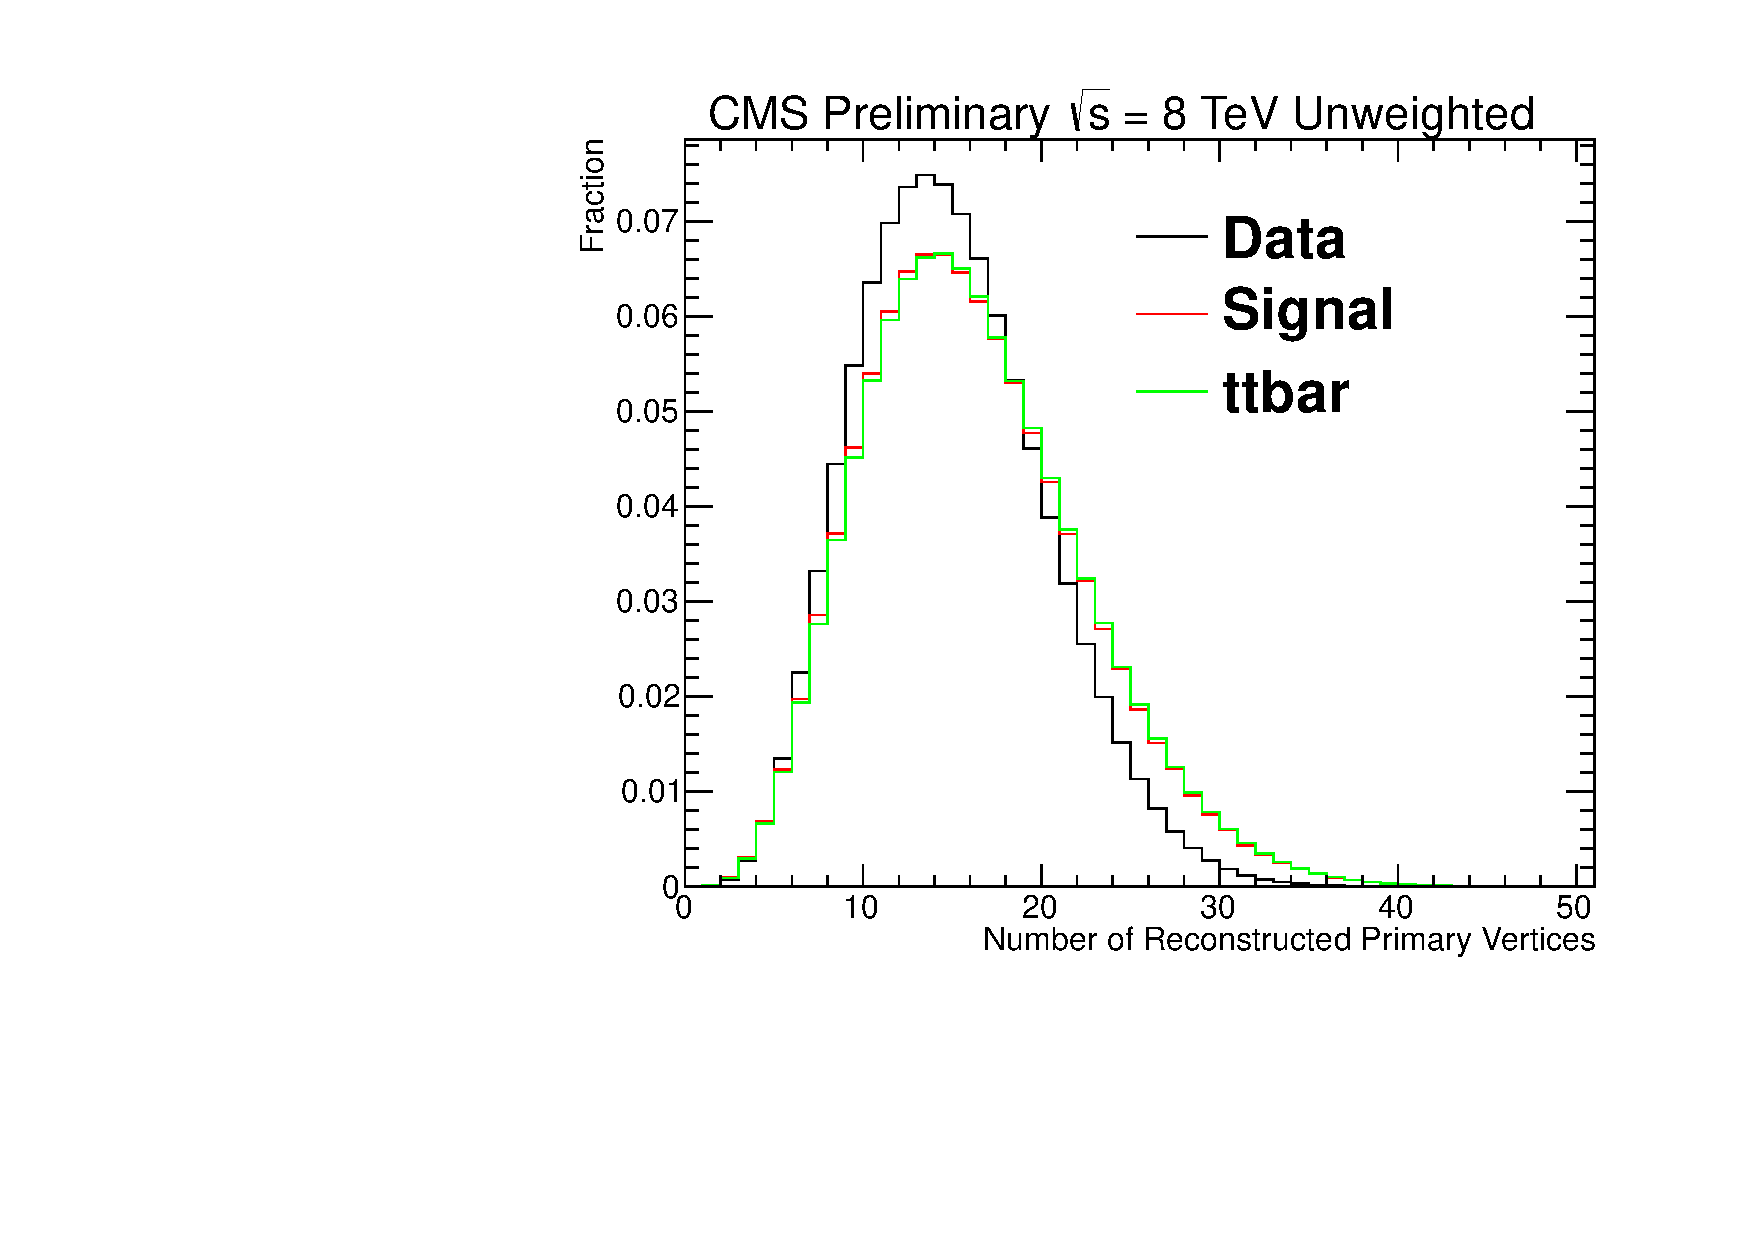
\includegraphics[width=0.7\linewidth]{AN-13-004/figs/npvuw.pdf}\\
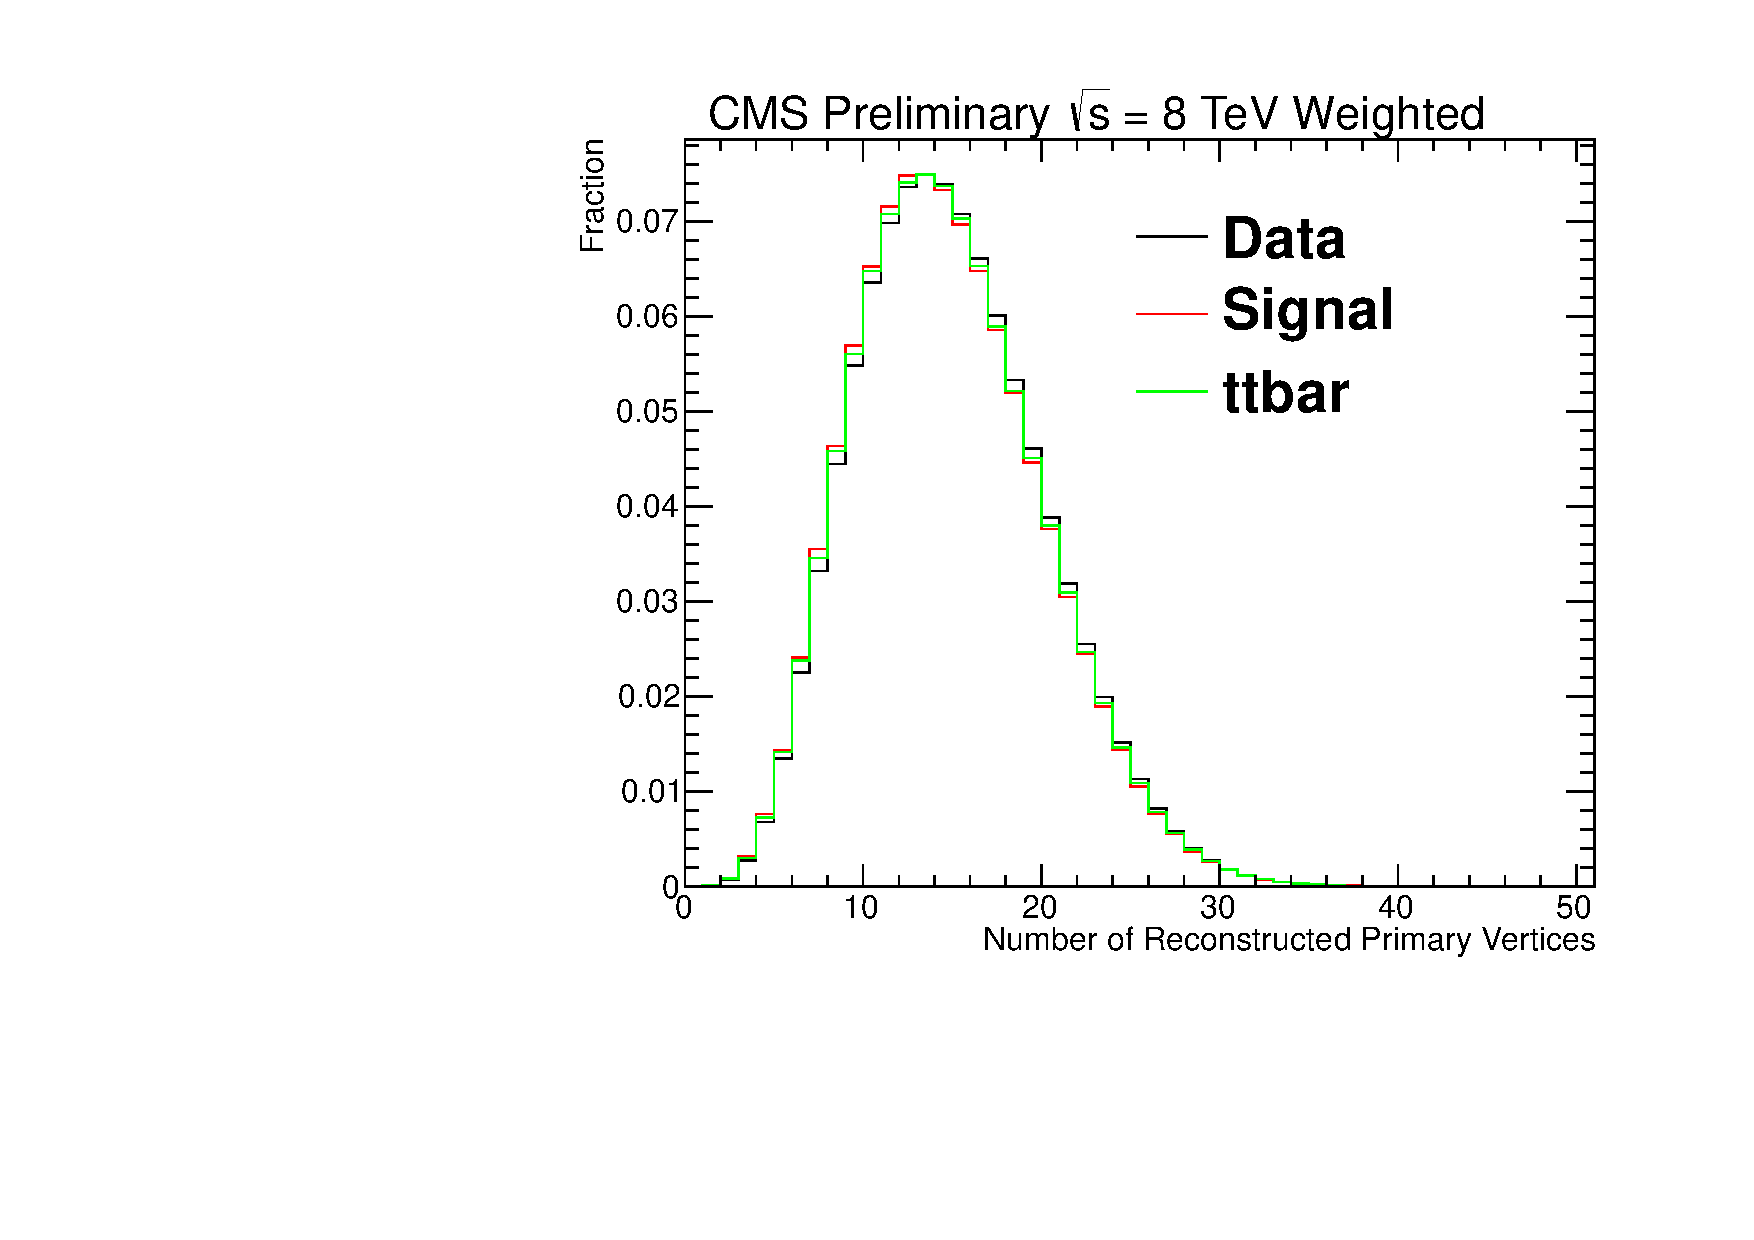
\includegraphics[width=0.7\linewidth]{AN-13-004/figs/npvw.pdf}
\end{center}
\caption{Number of reconstructed primary vertices before pileup re-weighting (top) and after pileup re-weighting (bottom).  Here, no analysis cuts have been applied and the signal mass point is 1900$~\GeV$}
\label{figs:npvweight}
\end{figure}

\begin{figure}[htcb]
\centering
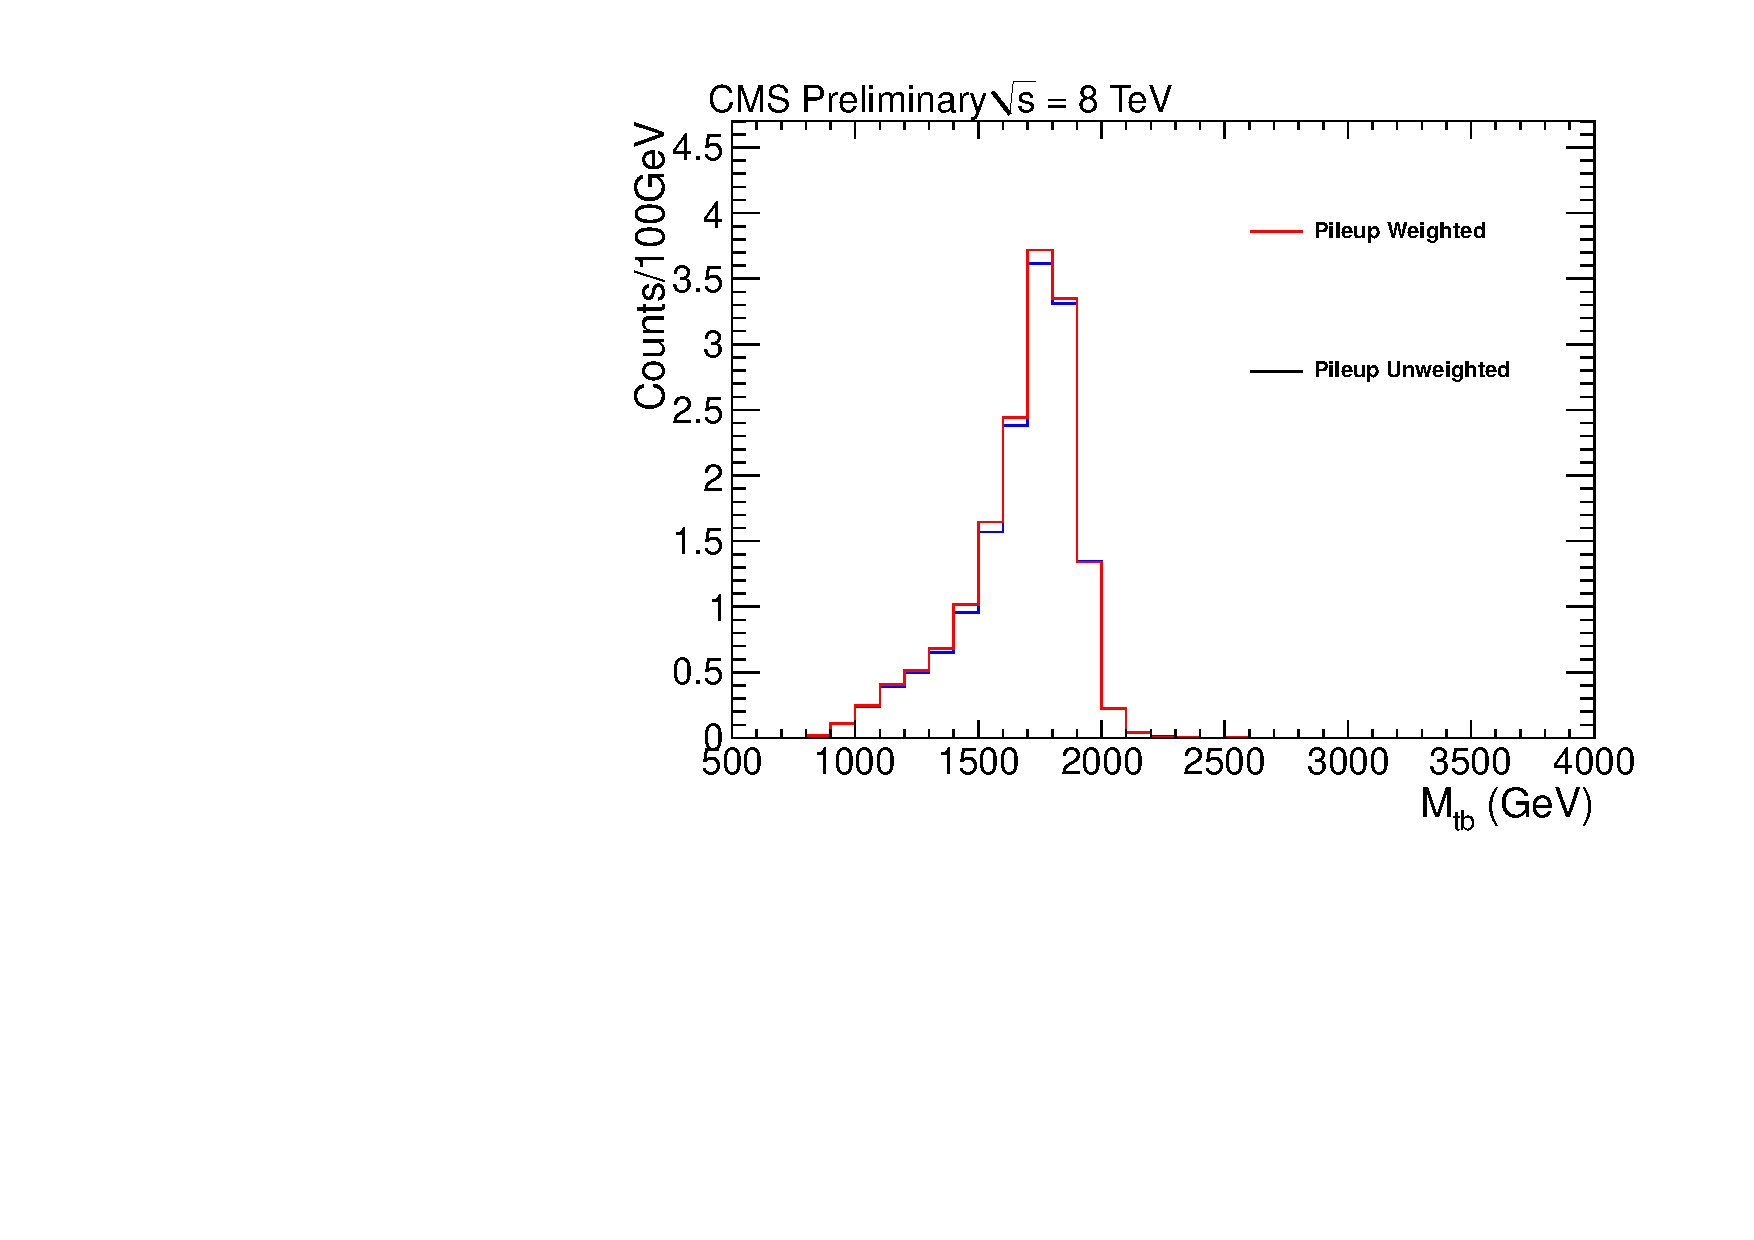
\includegraphics[width=0.9\textwidth]{AN-13-004/figs/Signal_M1900_PileupComp.pdf}
\caption{Effect of pileup-re-weighting on the Signal MC.}
\label{figs:pileup3}
\end{figure}

\begin{figure}[htcb]
\centering
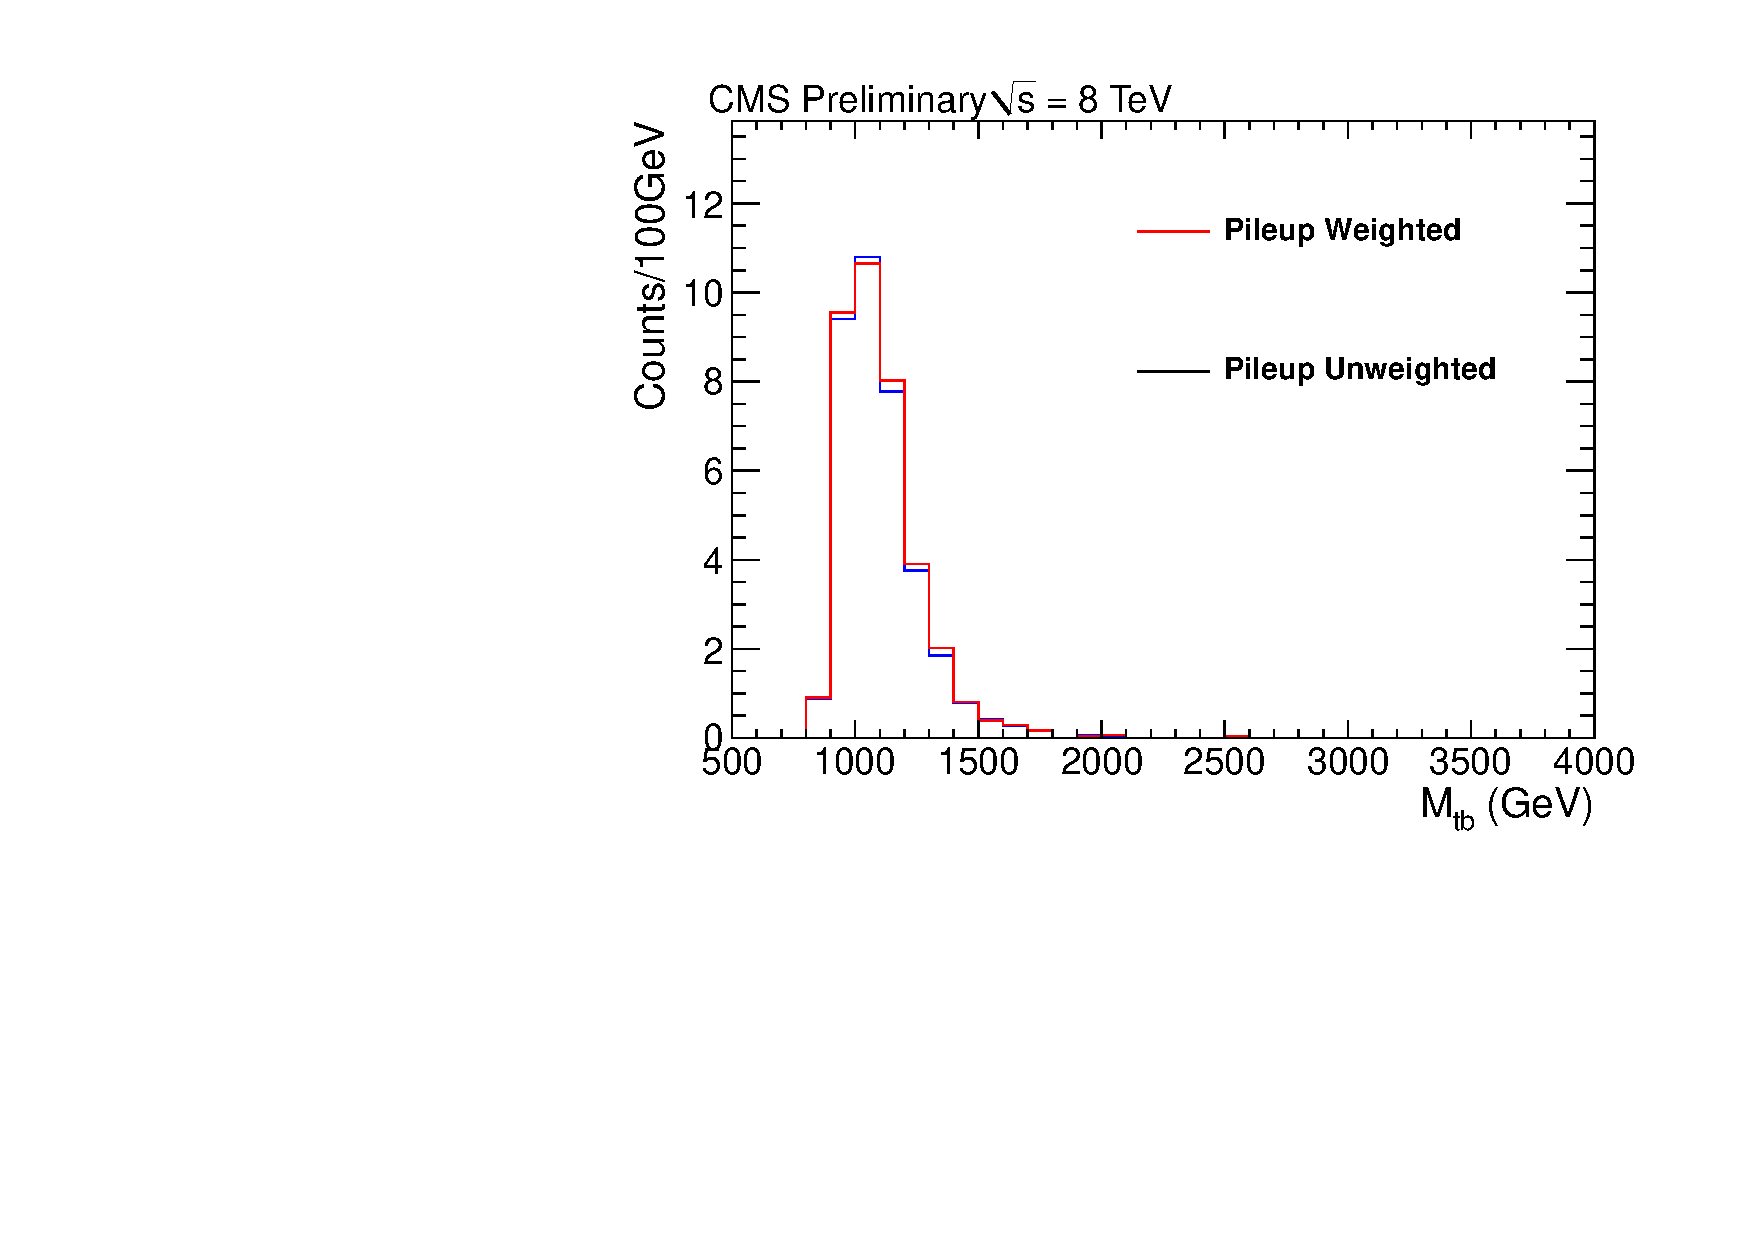
\includegraphics[width=0.9\textwidth]{AN-13-004/figs/TTbar_PileupComp.pdf}
\caption{Effect of pileup-re-weighting on the $\ttbar$ MC.}
\label{figs:pileup3ttbar}
\end{figure}



\subsection{Combined CMS Top Tagging Algorithm}
\label{sec:toptagging}
\label{sec:subjetSF}

The CMS top tagging algorithm takes CA jets with $R = 0.8$ as input.  
The algorithm first attempts to decompose the CA jet into two primary subjets, and then 
performs a secondary decomposition to attempt to split the subjets into secondary subjets \cite{JME13007}.
In this process, particles with low $\pt$ or a large angular distance from the jet center are omitted.
The top tagging algorithm is based on the following cuts

\begin{itemize}
\item {\bf Jet Mass}  $\mathrm{\boldmath 140~\GeV < m_{\text{jet}} < 250~\GeV}$ - The mass of the CA jet is required to be consistent with the top quark mass. 
\item {\bf Number of Subjets}  $\mathrm{\boldmath N_{\text{subjets}} > 2}$ - The number of subjets found by the algorithm must be at least 3.
\item {\bf Minimum Pairwise Mass} $\mathrm{\boldmath m_{\text{min}} > 50~\GeV}$  - The three highest $\pt$ subjets are
taken pairwise, and each pair's invariant mass is calculated. $m_{\text{min}}$ is the mass of the pair with the lowest invariant mass. The minimum pairwise mass must be close to the W mass.   
\end{itemize}
Figure \ref{figs:CutCompP} shows the comparison of Signal and QCD MC for the above top tagging selection. Here, the N-subjettiness and subjet b-tagging cuts are not applied.

\begin{figure}[htb]
\centering
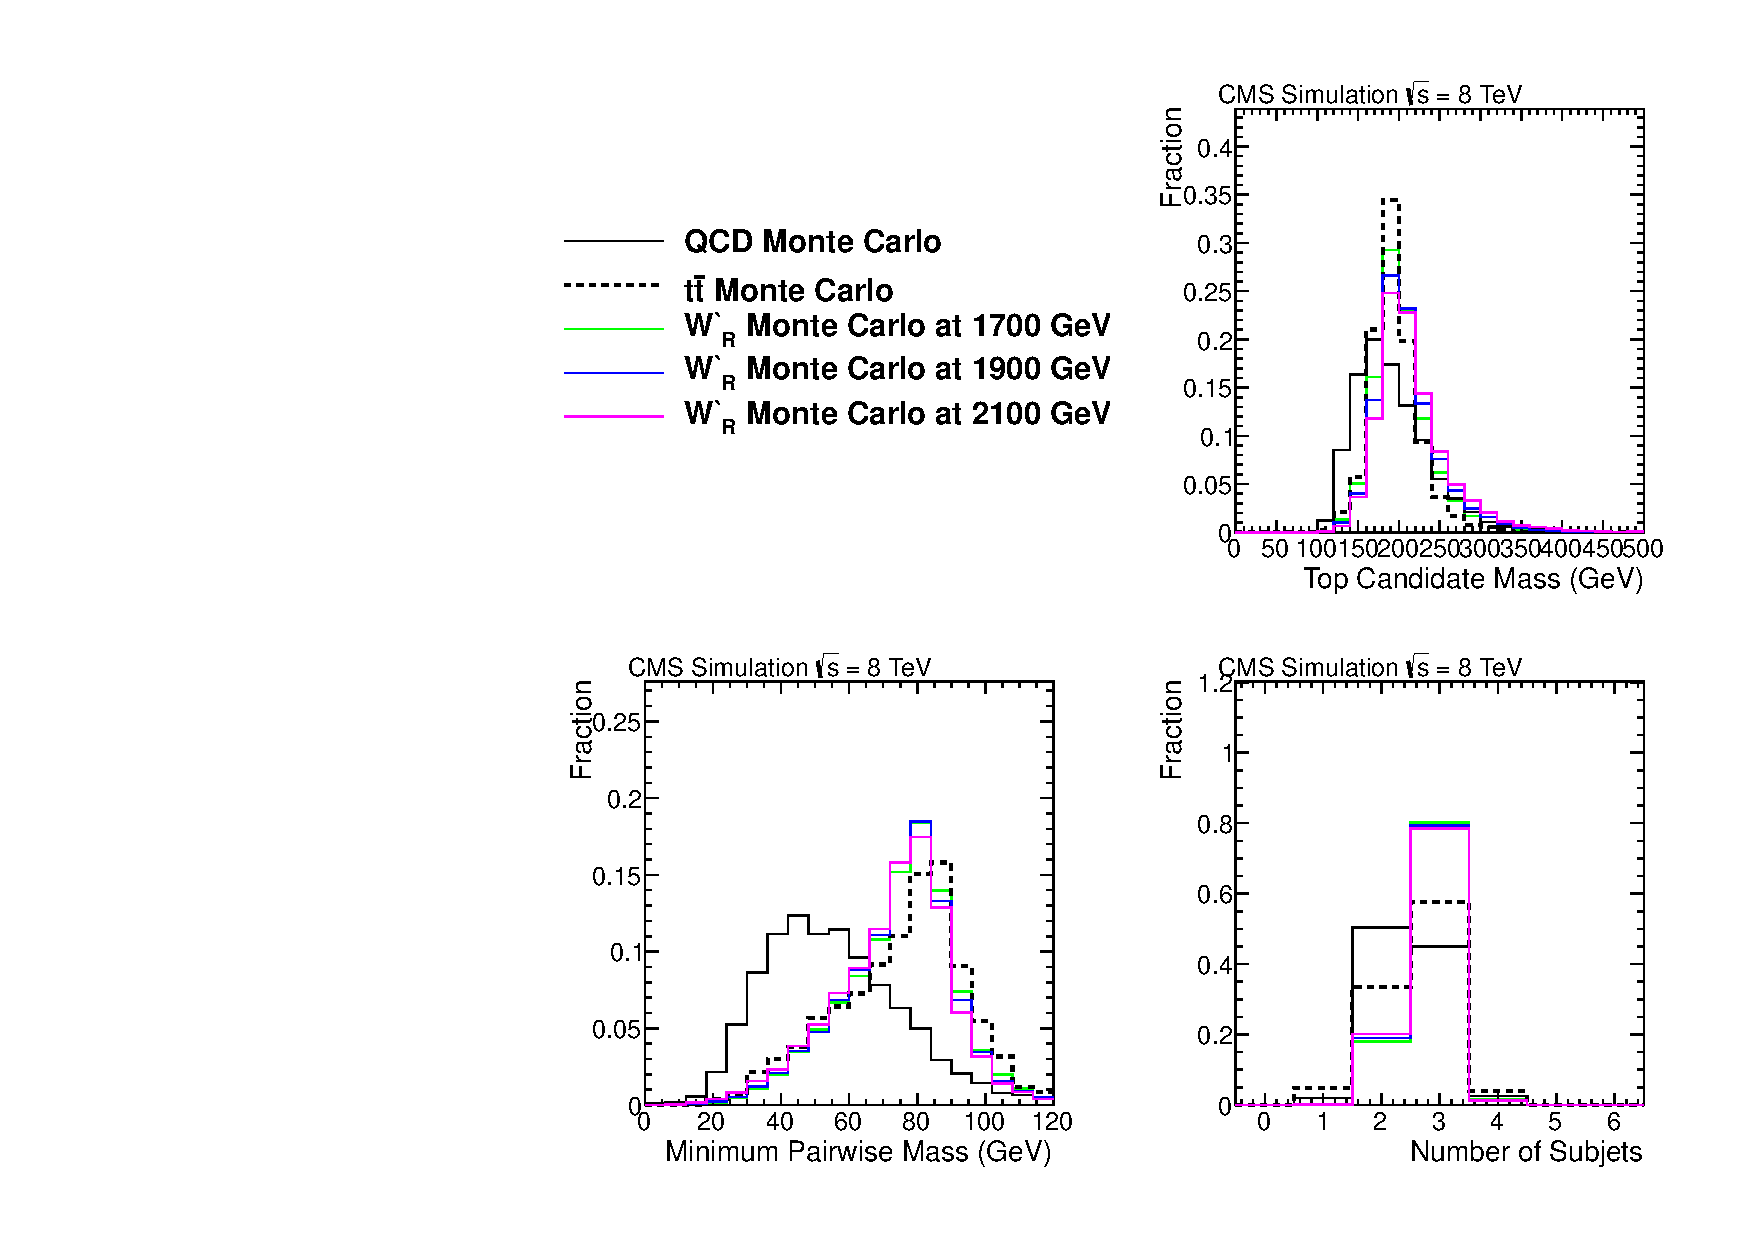
\includegraphics[width=1.0\textwidth]{AN-13-004/figs/CutCompqcdandsignal}
\caption{Comparison of the top Jet Mass, Number of Subjets, and Minimum Pairwise Mass in Signal and QCD MC.  The cms top tagging selection is applied 
with the exception of the variable being plotted.}
\label{figs:CutCompP}
\end{figure}

The N-subjettiness algorithm can be used for boosted top jet identification \cite{Thaler:2011gf}.  N-subjettiness defines $\tau_N$ variables as follows 
\begin{eqnarray}
	\mathrm{\tau_{N} = \frac{1}{d_0}\sum_{i}p_{T_i}min\{\Delta R_{1,i},\Delta R_{2,i},...,\Delta R_{N,i}\}}
\end{eqnarray}
where $\Delta R_{J,i}$ is between the subjet candidate and a constituent particle.  $d_0$ is a normalization factor 
\begin{eqnarray}
	\mathrm{d_0 = \sum_i p_{T_i} R_0}
\end{eqnarray}
where $\mathrm{R_0}$ is the characteristic jet radius used by the jet clustering algorithm.  For this analysis we use the one pass kt method of subjet axes minimization.  $\mathrm{\tau_N}$ is a measure of how consistent the jet energy is with originating from N subjets. 
Additional discrimination power when using N-subjettiness variables is achieved by cutting on the ratio of two of these variables.   
Figure \ref{figs:NsubCOMP} shows $\mathrm{\tau_3/\tau_2}$ comparison using signal and QCD MC samples.  We use the standard operating point of $\mathrm{\tau_3/\tau_2} < 0.55$  \cite{JME13007} in the full selection.

\begin{figure}[htcb]
\begin{center}
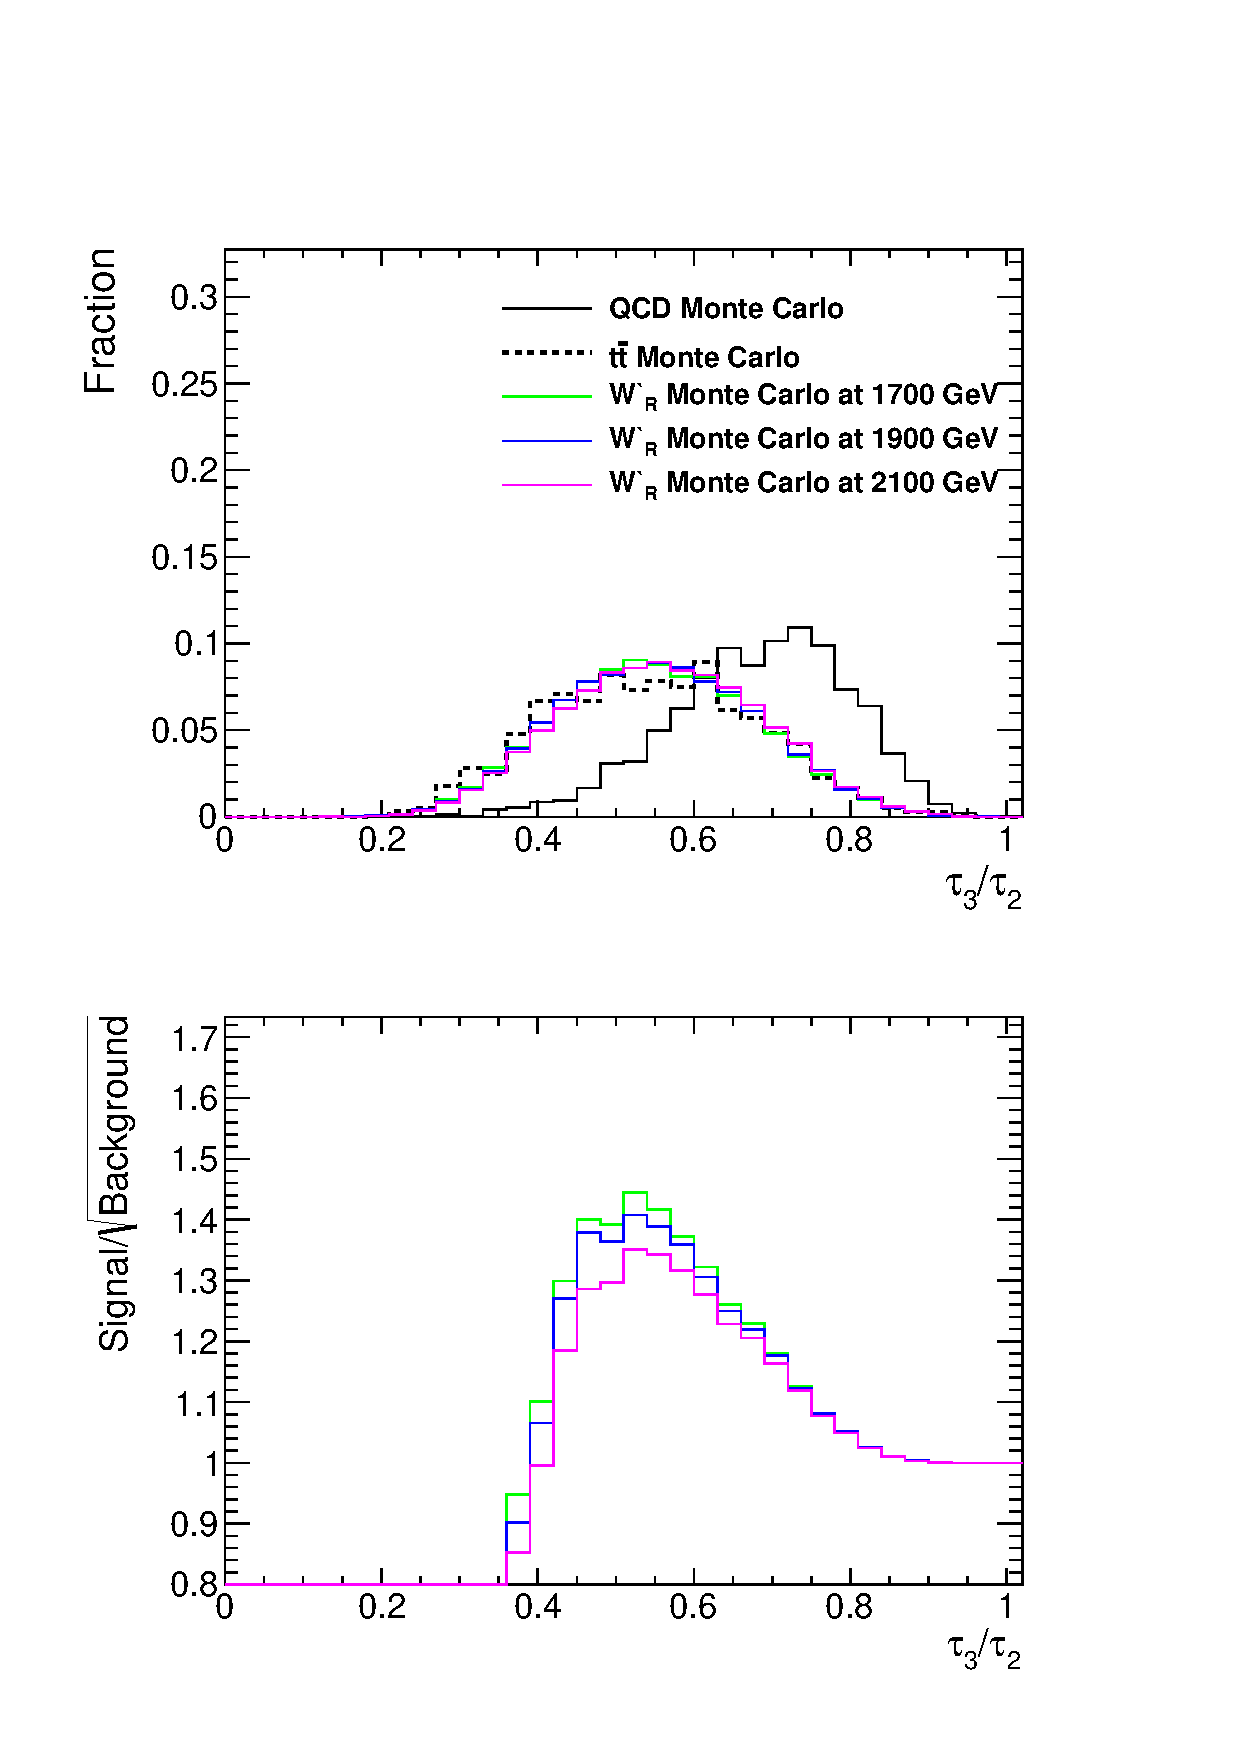
\includegraphics[width=0.7\textwidth]{AN-13-004/figs/tau32Compqcdandsignal.pdf}
\caption{
$\mathrm{\tau_3/\tau_2}$ distributions in Signal and QCD MC samples (top).  Plot of Signal/$\sqrt{\text{Background}}$ (bottom), derived from the top plot.
}
\label{figs:NsubCOMP}
\end{center}
\end{figure}

The use of b-tagging algorithms on subjets is described in \cite{CMS-PAS-BTV-13-001}.  We apply the Combined Secondary Vertex b-tagging algorithm 
to all of the subjets found by the CA declustering sequence described 
above.  The optimal discrimination variable when using subjet b-tagging is the maximum discriminant out of the three or four subjets found.  
Figure \ref{figs:BtagCOMP} shows the maximum subjet CSV b discriminant comparison using signal and QCD MC samples.  We use the standard CSV working point $SJ_{\text{CSVMAX}} > 0.679$.

\begin{figure}[htcb]
\begin{center}
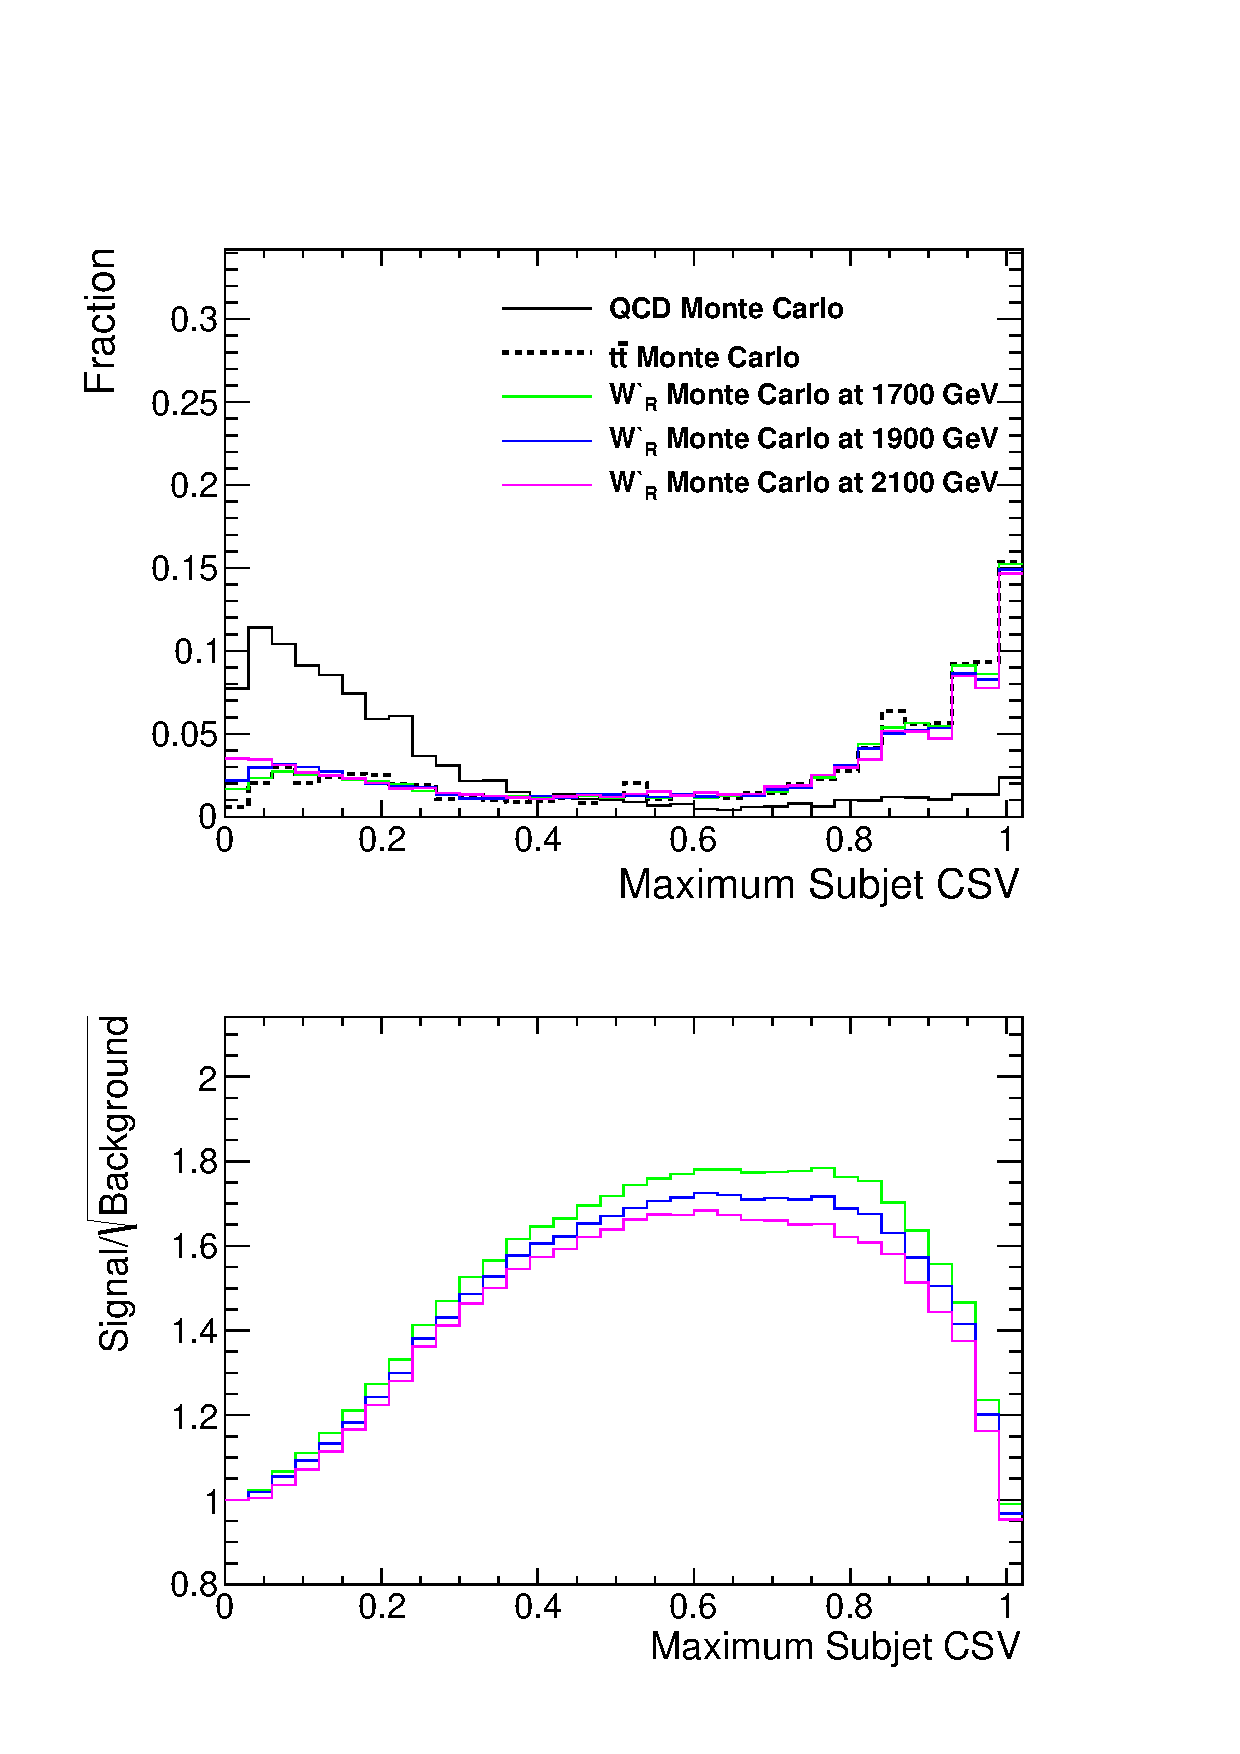
\includegraphics[width=0.7\textwidth]{AN-13-004/figs/bmaxCompqcdandsignal.pdf}
\caption{
Maximum subjet CSV distributions in Signal and QCD MC samples (top).  Plot of Signal/$\sqrt{\text{Background}}$ (bottom), derived from the top plot. 
}
\label{figs:BtagCOMP}
\end{center}
\end{figure}

Substructure variables in the signal region have known differences in data and MC \cite{JME13007}.  
We use the top tagging scale factor with the addition of subjet b-tagging and N-subjettiness discrimination that is extracted 
from efficiency comparisons of data and MC in a highly pure semileptonic $\ttbar$ sample.   
The scale factor for this effect is 1.04 and is applied to the signal MC samples used in the main analysis.  
There is a 13\% uncertainty on this scale factor which is purely statistical, as the study is dominated by statistical uncertainty.  
The scale factor is obtained from the plots shown in Figure \ref{figs:type1_topmasspowheg}.

\begin{figure}
\begin{center}
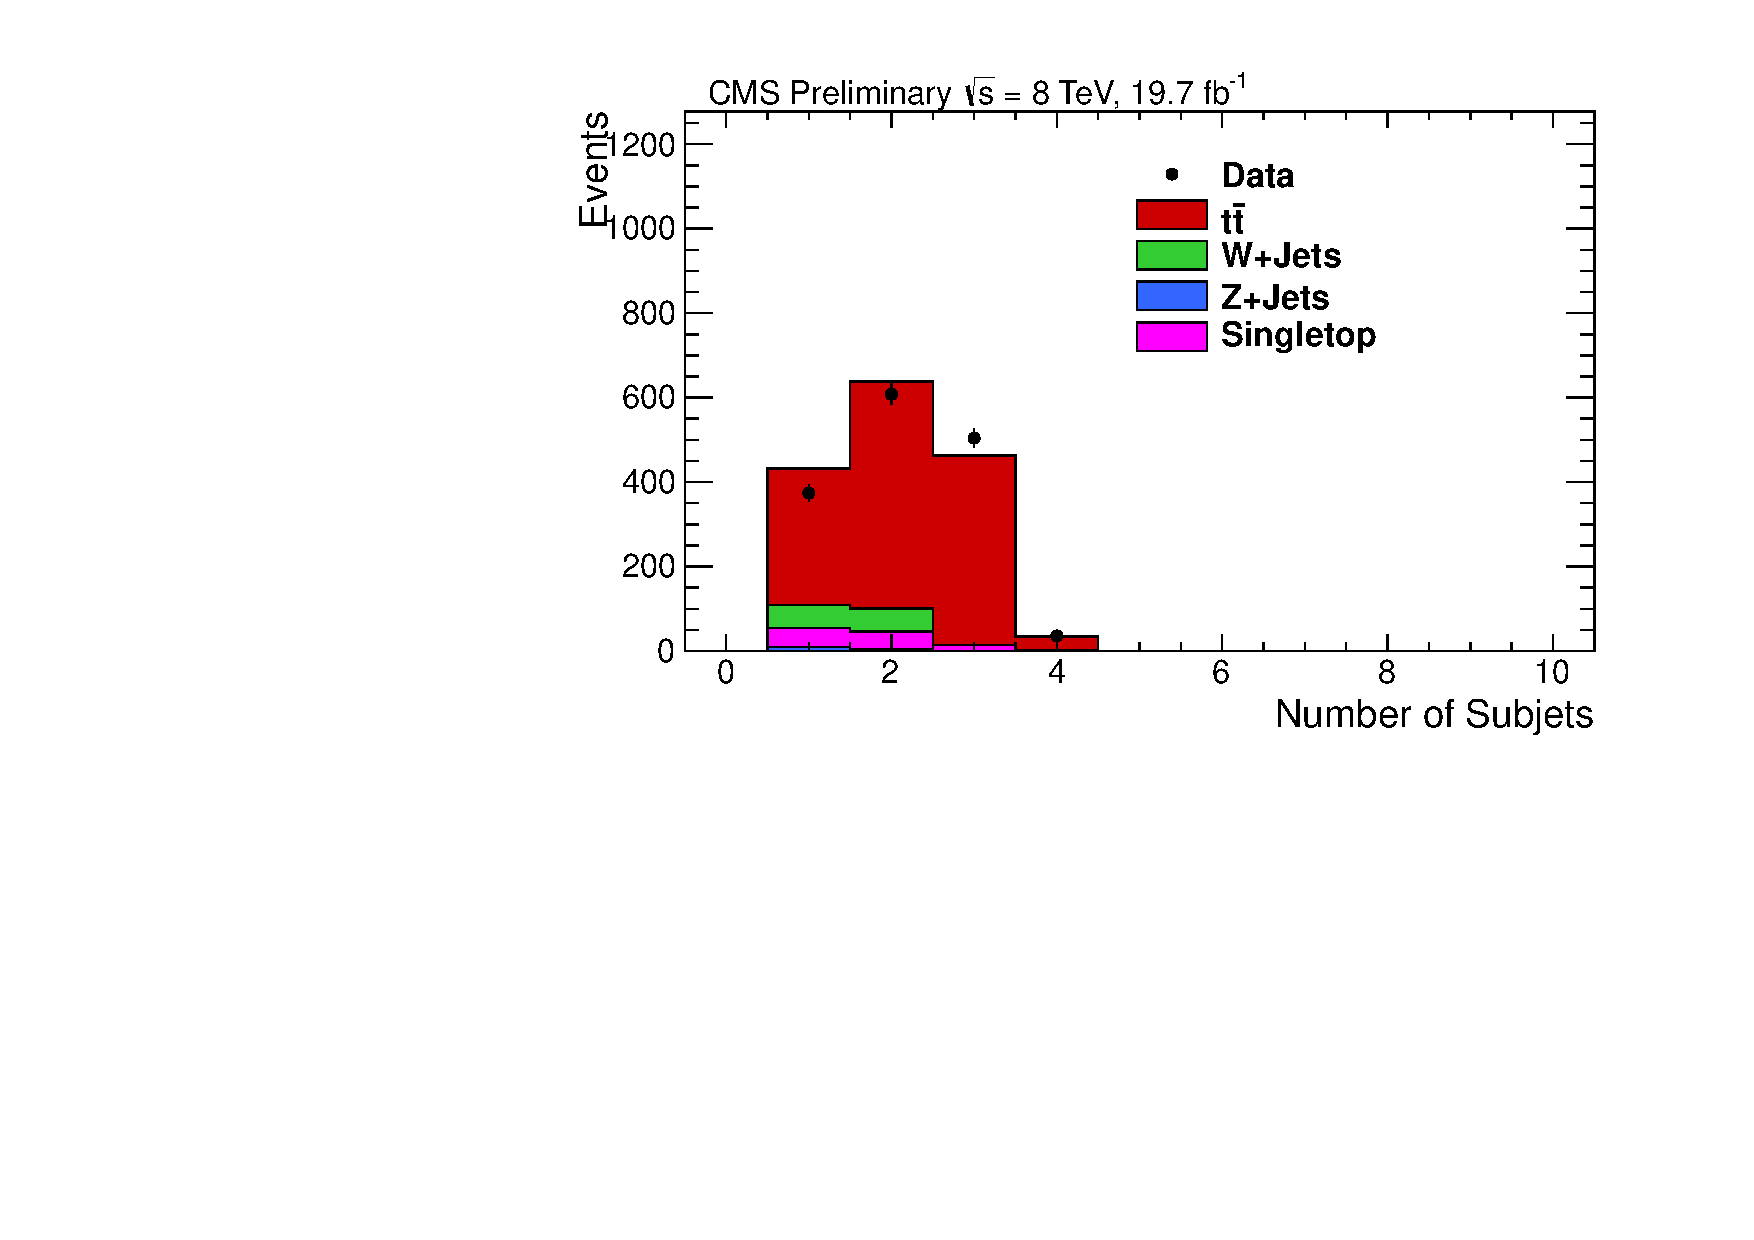
\includegraphics[width=0.45\linewidth]{AN-13-004/figs/semiLepMass_t1Nsubjets_POWHEG_TTWeight.pdf}
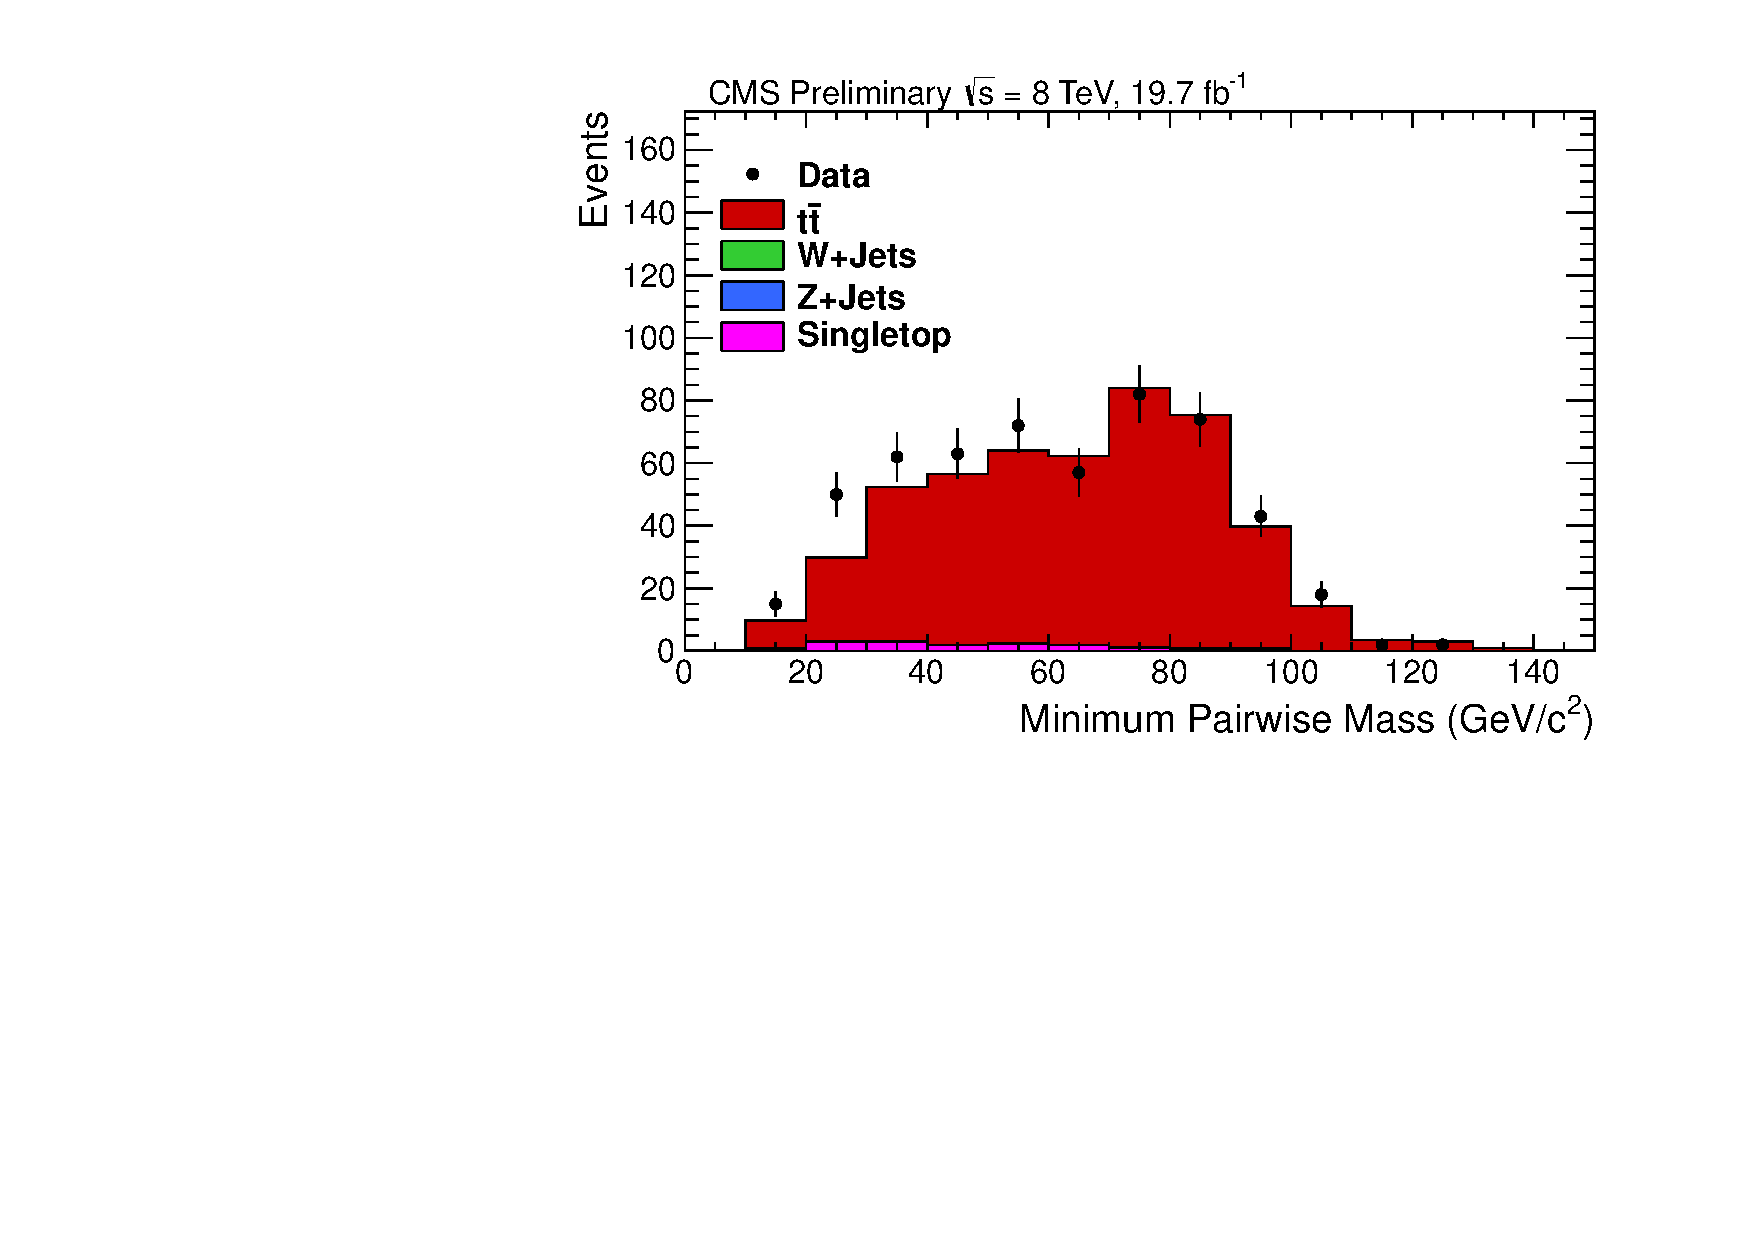
\includegraphics[width=0.45\linewidth]{AN-13-004/figs/semiLepMass_t1MinimumPairwiseMass_POWHEG_TTWeight.pdf}\\
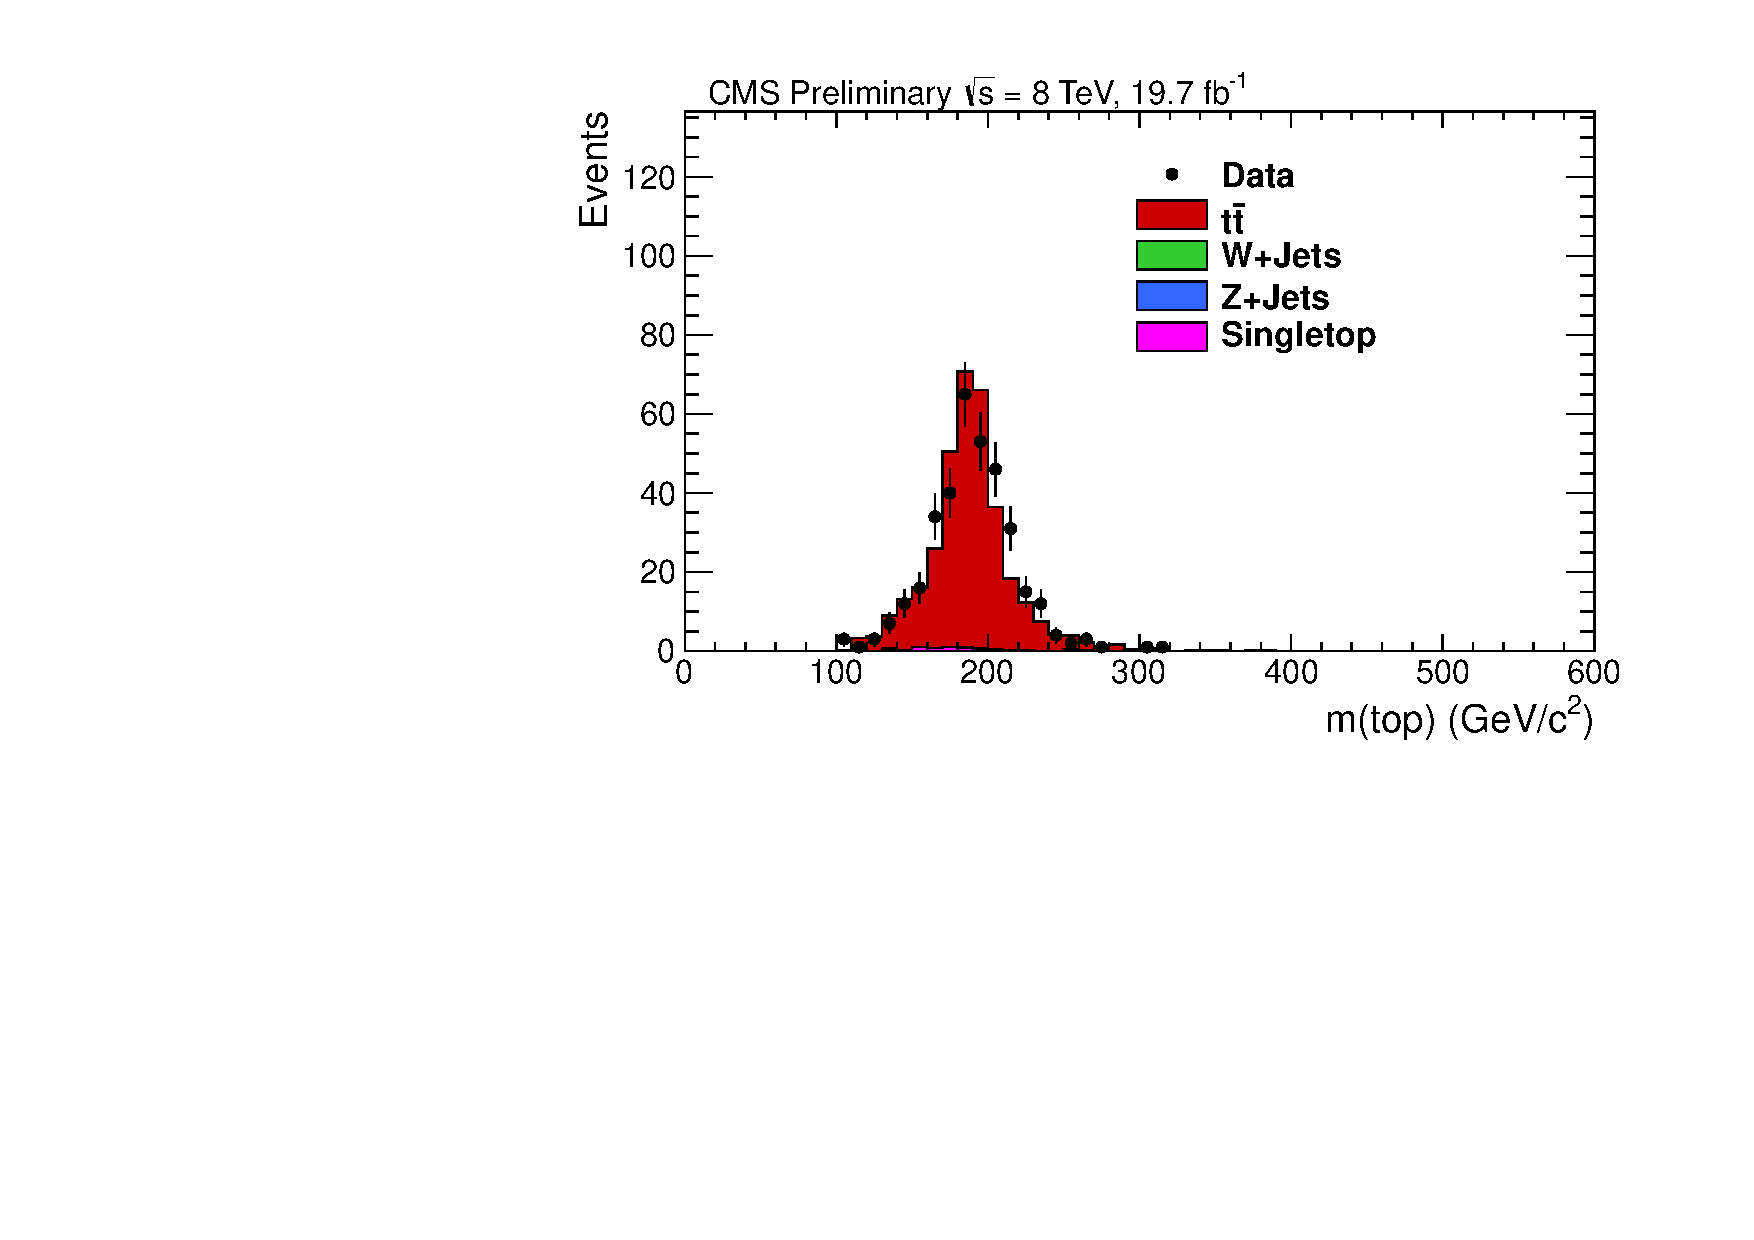
\includegraphics[width=0.45\linewidth]{AN-13-004/figs/semiLepMass_t1TopMass_POWHEG_TTWeight.pdf}
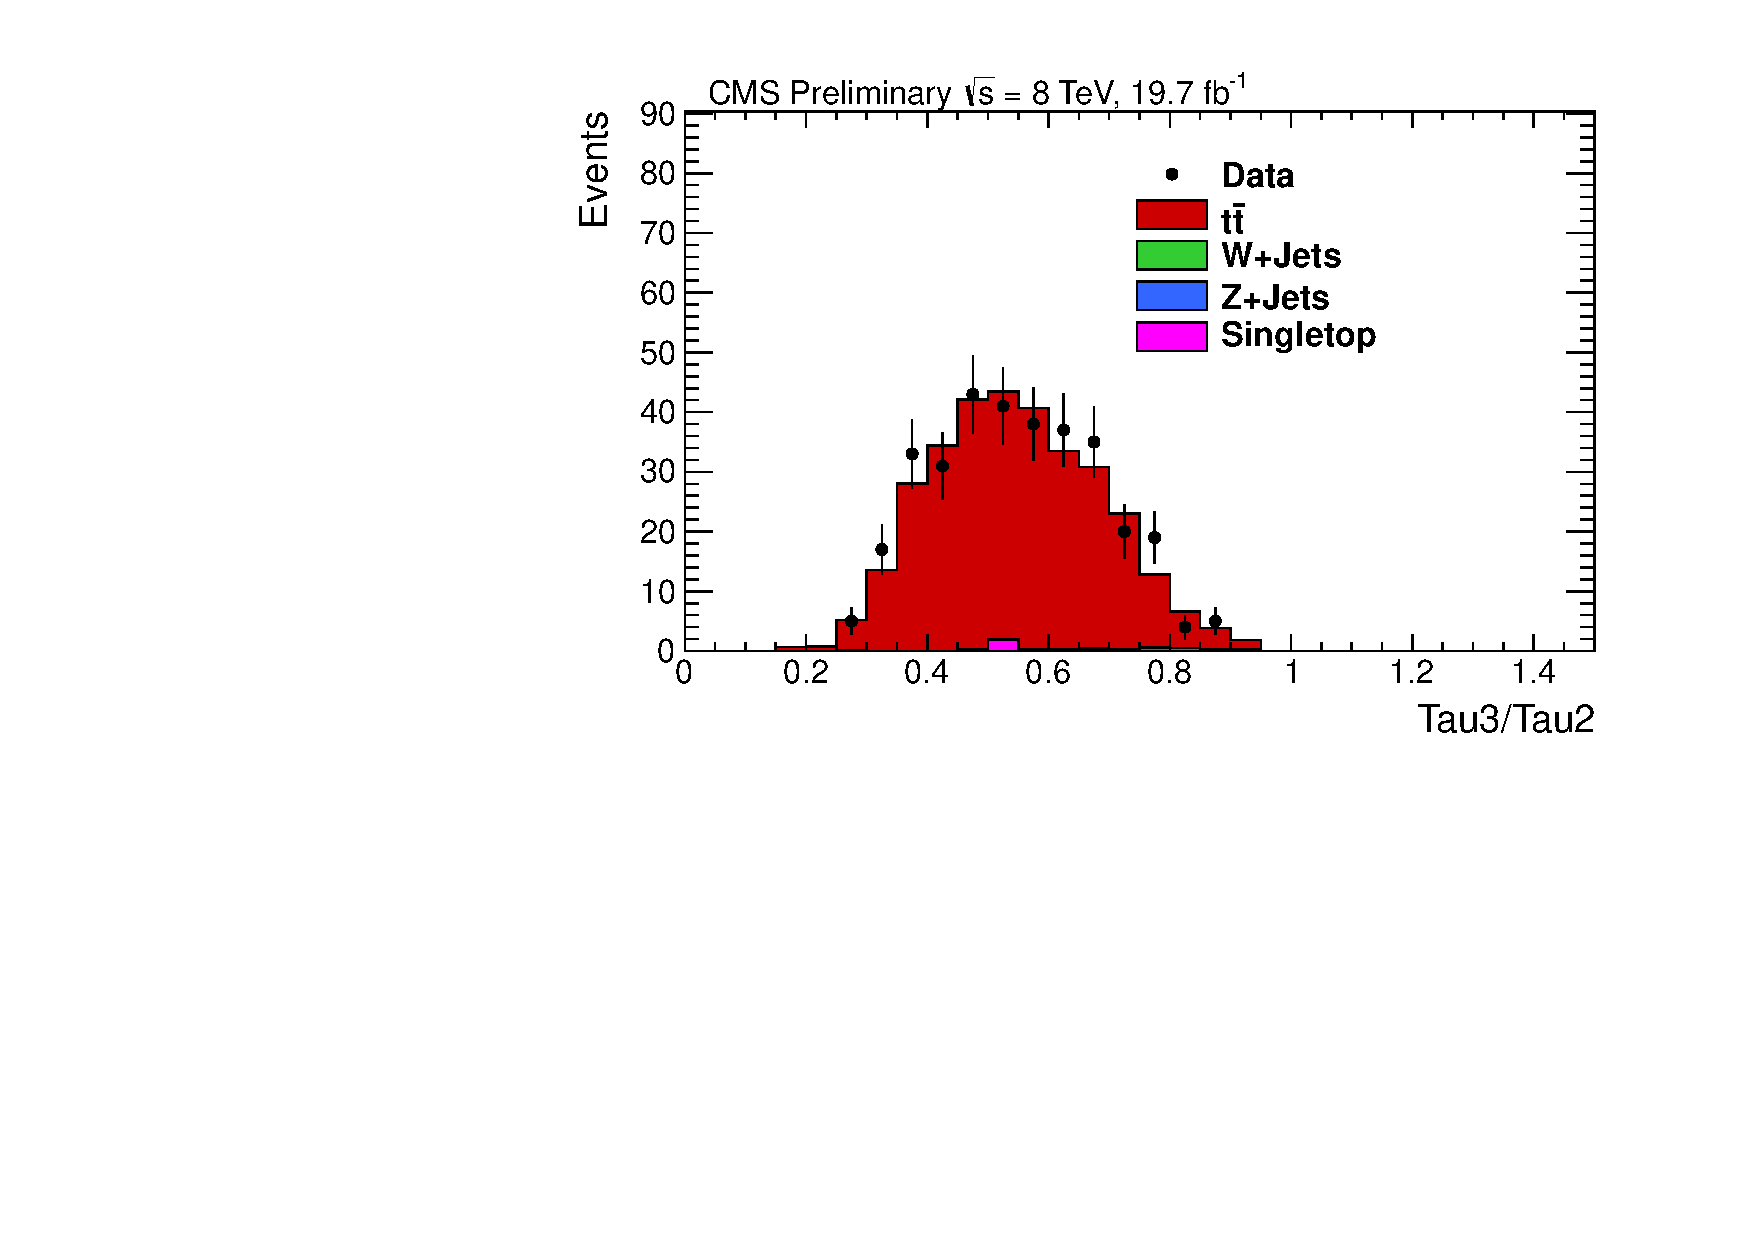
\includegraphics[width=0.45\linewidth]{AN-13-004/figs/semiLepMass_t1Tau32_POWHEG_TTWeight.pdf}\\
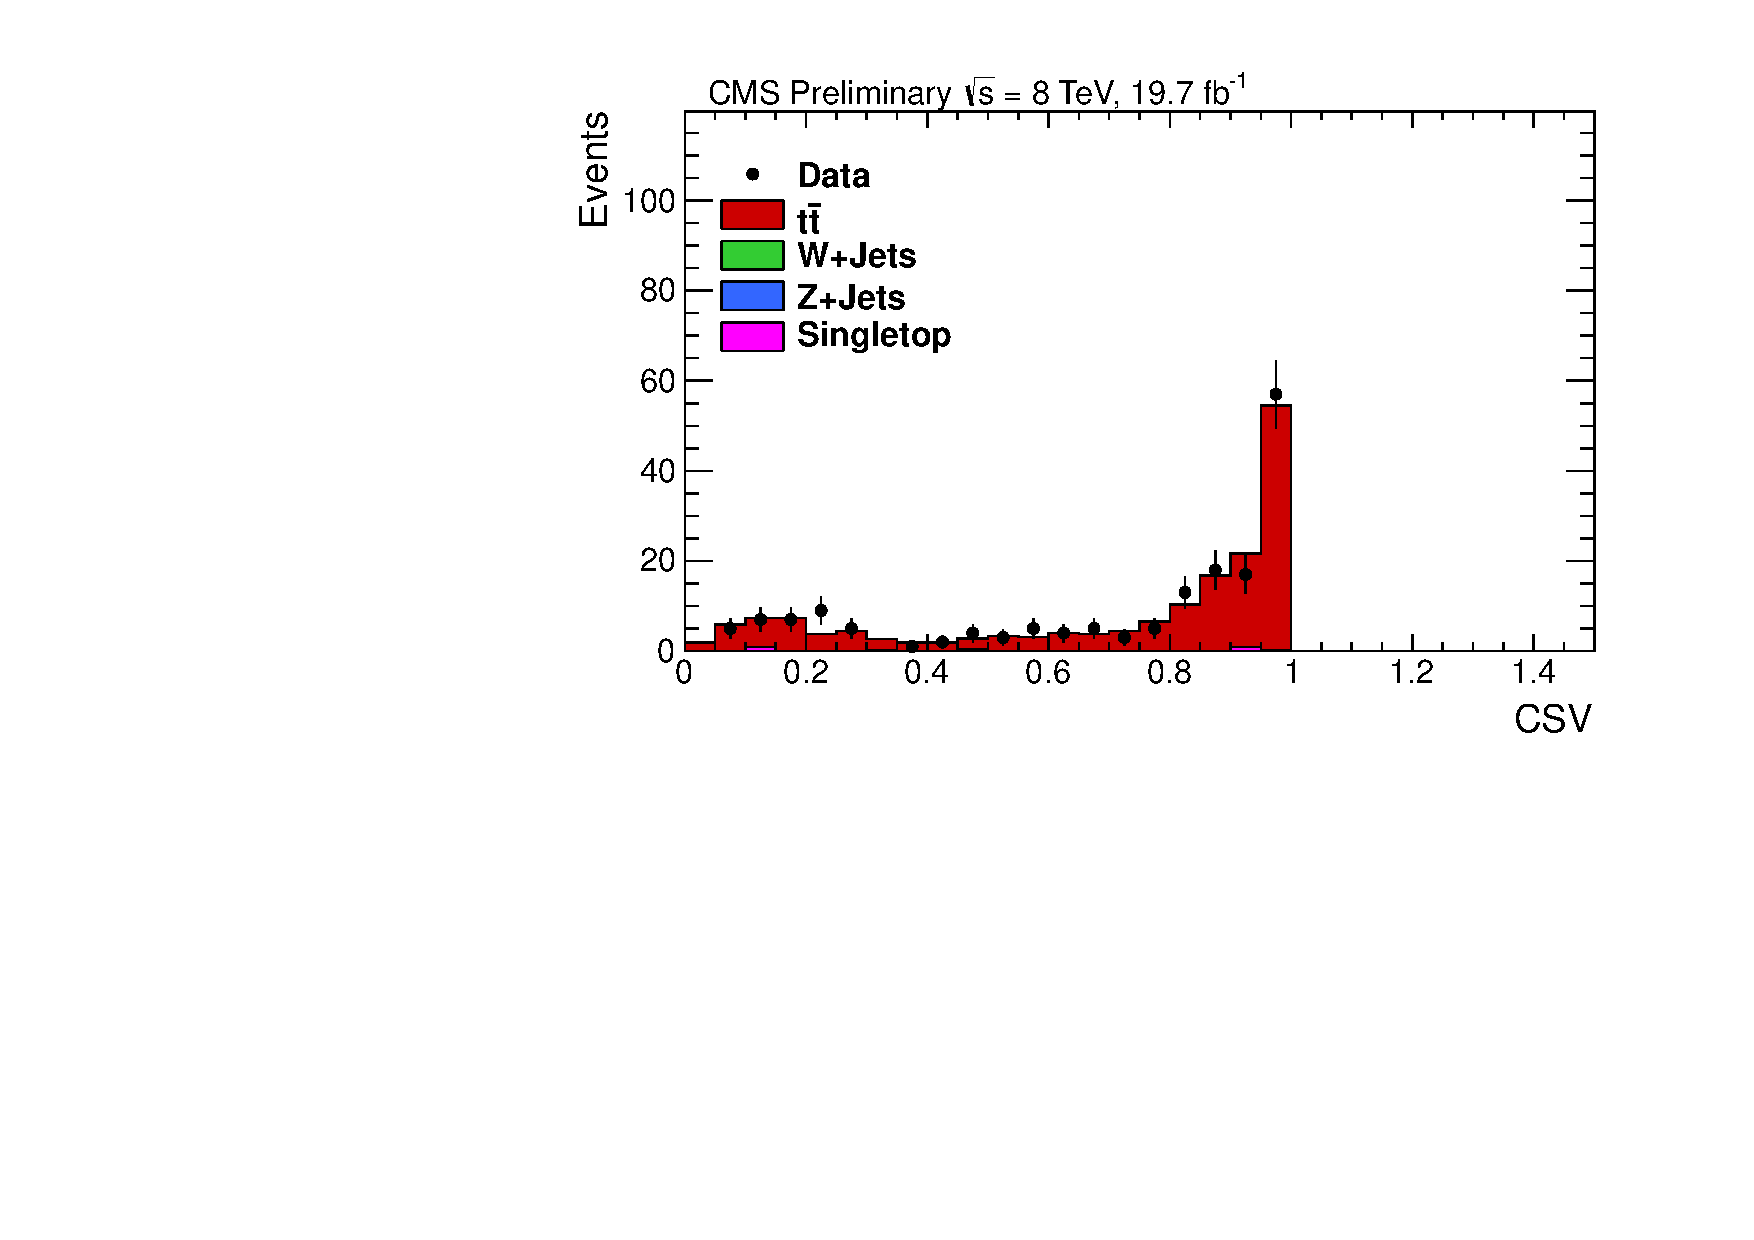
\includegraphics[width=0.45\linewidth]{AN-13-004/figs/semiLepMass_t1BMax_POWHEG_TTWeight.pdf}
\end{center}
\caption{ a.)Number of subjets, b.)minimum pairwise subjet mass, c.)jet mass, d.)$\mathrm{\tau_{3}/\tau_{2}}$, and  e.)maximum subjet CSV for fully-merged top candidates
  found in the semileptonic $\ttbar$ sample, used to evaluate the top-tagging efficiency SF.  These Figures are extracted using the Powheg $\ttbar$ MC Sample. }%  The shaded regions represent the total uncertainty on the background model.}
\label{figs:type1_topmasspowheg}
\end{figure}

\subsection{Delta Rapidity Cut}
\label{sec:deltarapidity}
At high $\mathrm{M_{\tbbar}}$, jets that originate from QCD multijet production are widely separated in rapidity (high $\Delta y$).
However the jets originating from a high mass $\tbbar$ resonance do not exhibit such pronounced separation.  The effect is not pronounced over the entire 
$\mathrm{M_{\tbbar}}$ spectrum, but for high values of $\mathrm{M_{\tbbar}}$ the analysis can achieve greater separation of signal and background.  We therefore place a cut on $|\Delta y| < 1.6$ 
for the full selection.  The value for this cut was chosen by investigating the Signal/$\sqrt{\text{Background}}$ distribution in events that have $\mathrm{M_{\tbbar}}>2000~\GeV$.  
Because it is not as effective over the entire $\mathrm{M_{\tbbar}}$ range, the value is set slightly off the peak to minimize loss of signal efficiency.
%The value of 1.6 was determined by optimizing $S/\sqrt{B}$ where $S$ is the number of events in the signal region and $B$ is the number of events attributed to background in the region of interest for each signal mass point.  The cut value was chosen based on maximizing the expected counting experiment limit described in Section \ref{sec:countingexperiment}.  
Figure \ref{figs:CutComp} shows the comparison of $|\Delta y|$ for high $\mathrm{M_{\tbbar}}$ in signal and QCD MC.  
Here, the N-subjettiness and subjet b-tagging cuts are not applied.
% Additionally, the lowest $\pt$ QCD MC sample has poor statistics for the high $\mathrm{M_{tb}}$ region and is not included in this figure.

\begin{figure}[htb]
\centering
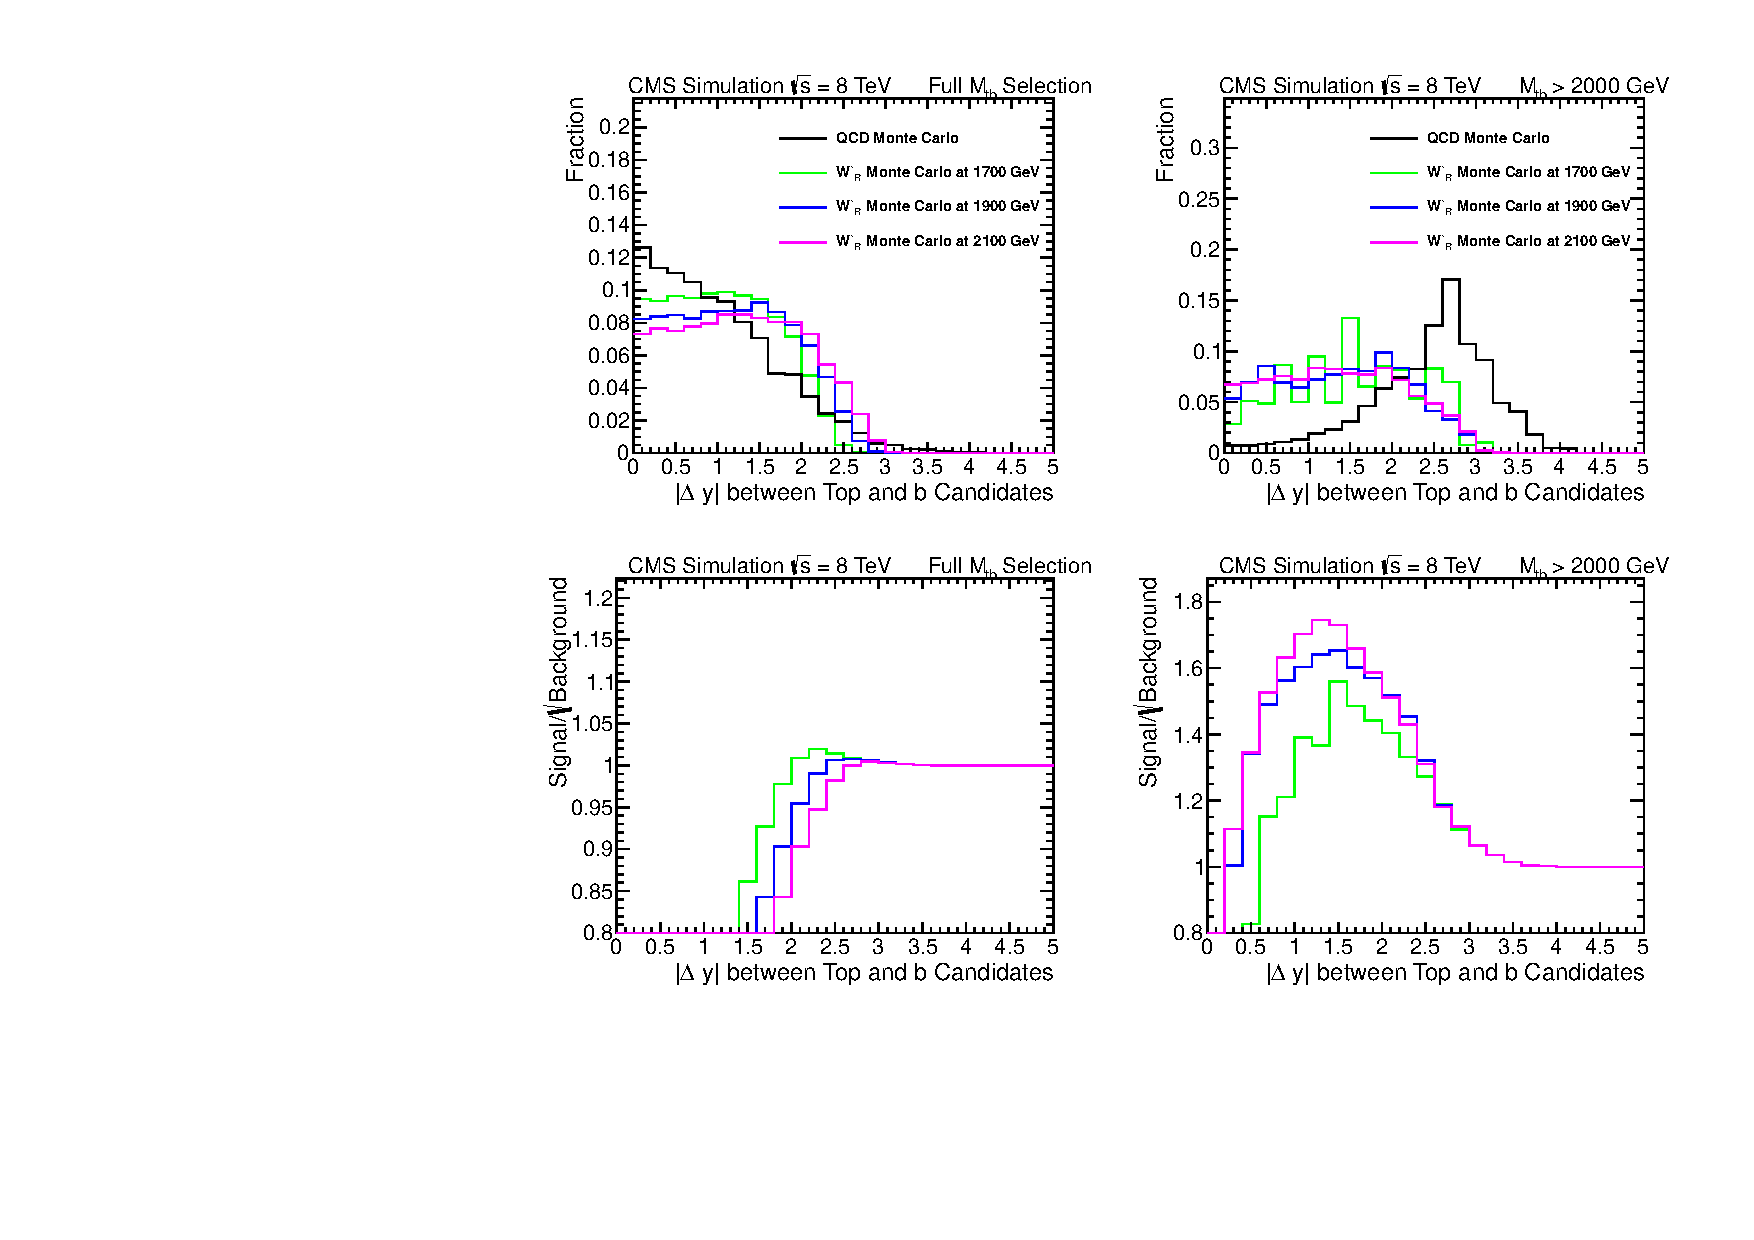
\includegraphics[width=1.0\textwidth]{AN-13-004/figs/drapCompqcdandsignal}
\caption{Comparison of $|\Delta y|$ in signal and QCD MC for the full selection and only events with $\mathrm{M_{\tbbar}} > 2000~\GeV$}
\label{figs:CutComp}
\end{figure}



\subsection{b-jet Identification}
\label{sec:btagging}
To enhance the sensitivity of the analysis, the Combined Secondary Vertex (CSV) b-tagging algorithm is applied to the subleading jet. We use the standard operating point CSVM (CSV $>$ 0.679).
%after optimizing S/$\sqrt{B}$ using all 8TeV supported b-tagging algorithms and operating points.  
Due to the fact that our signal content 
contains only $\tbbar$ and the only MC used in background estimation is $\ttbar$, the MC to data scale factor used in the analysis for b-tagging 
is the b-tagging Scale Factor for b quarks ($\mathrm{SF_b}$).  We use the suggested scale factor parameterized in $\pt$ with the following functional form for 
b candidate jet $\pt < 800~\GeV$

\begin{eqnarray}
\mathrm{SF_b = 0.938887 + 0.00017124\times \pt - 2.76366 \times 10^{-07} \times \pt^2} 
\end{eqnarray}
Any b candidate jet with $\pt > 800~\GeV$ is weighted with $\mathrm{SF_b}$ evaluated at 800$~\GeV$.  The parameterized $\mathrm{SF_b}$ is the 
suggested EPS13 prescription \cite{CMS-PAS-BTV-13-001} from the b-tagging POG generated from measurements in both muon-jet and ttbar data representing 20$~\fbinv$ of integrated 
luminosity. The uncertainty associated with this scale factor parameterization is described in Section \ref{sec:systematics}.  b-tagging operating points 
and scale factors have been validated for use with anti-kt jets with a R value of 0.5 (AK5 jets).  In our kinematic regime it is assumed that the change in cone size 
will have a small effect. We apply an additional $2\%$ systematic uncertainty to the signal MC samples used in the analysis. This is a conservative estimate of the uncertainty, validated by the following study: 

For the $2700~\GeV$ signal sample, we 
included both AK5 and CA8 jets in the event selection.  All jets considered were required to be in our pt range ($\pt > 350~\GeV$).  We attempt to match a CA8 jet to 
the corresponding AK5 jet using a constraint on $\eta$ and $\phi$ ($\Delta$R $< 0.3$ ).  The results were 579041 CA8 jets pass pt cut,
of these, 567155 pass the $\eta$ , $\phi$ matching to AK5 jets.  Of the matched jets, $96.9\%$ record the same value for the CSVM cut (pass or fail). In addition, 
the ratio of b-tagging efficiencies for both AK5 and CA8 were found to be within a $2\%$ deviation (see Figure \ref{figs:btageff}).  To rule out a bias based on the 
known differences in pt for CA8 and AK5 jets, the efficiencies and uncertainties were extracted from plots using only the pt of the CA8 jet.  
The fit on the b-tagging efficiency ratio for CA8 and AK5 jets can be interpreted as an upper bound on the uncertainty due to this effect.
We also checked this process for $1300~\GeV$ and $1900~\GeV$ signal samples and found results consistent with this $2\%$ error. 
We have verified this systematic uncertainty with the BTV group, and it is approved for use in our analysis.

\begin{figure}[htcb]
\centering
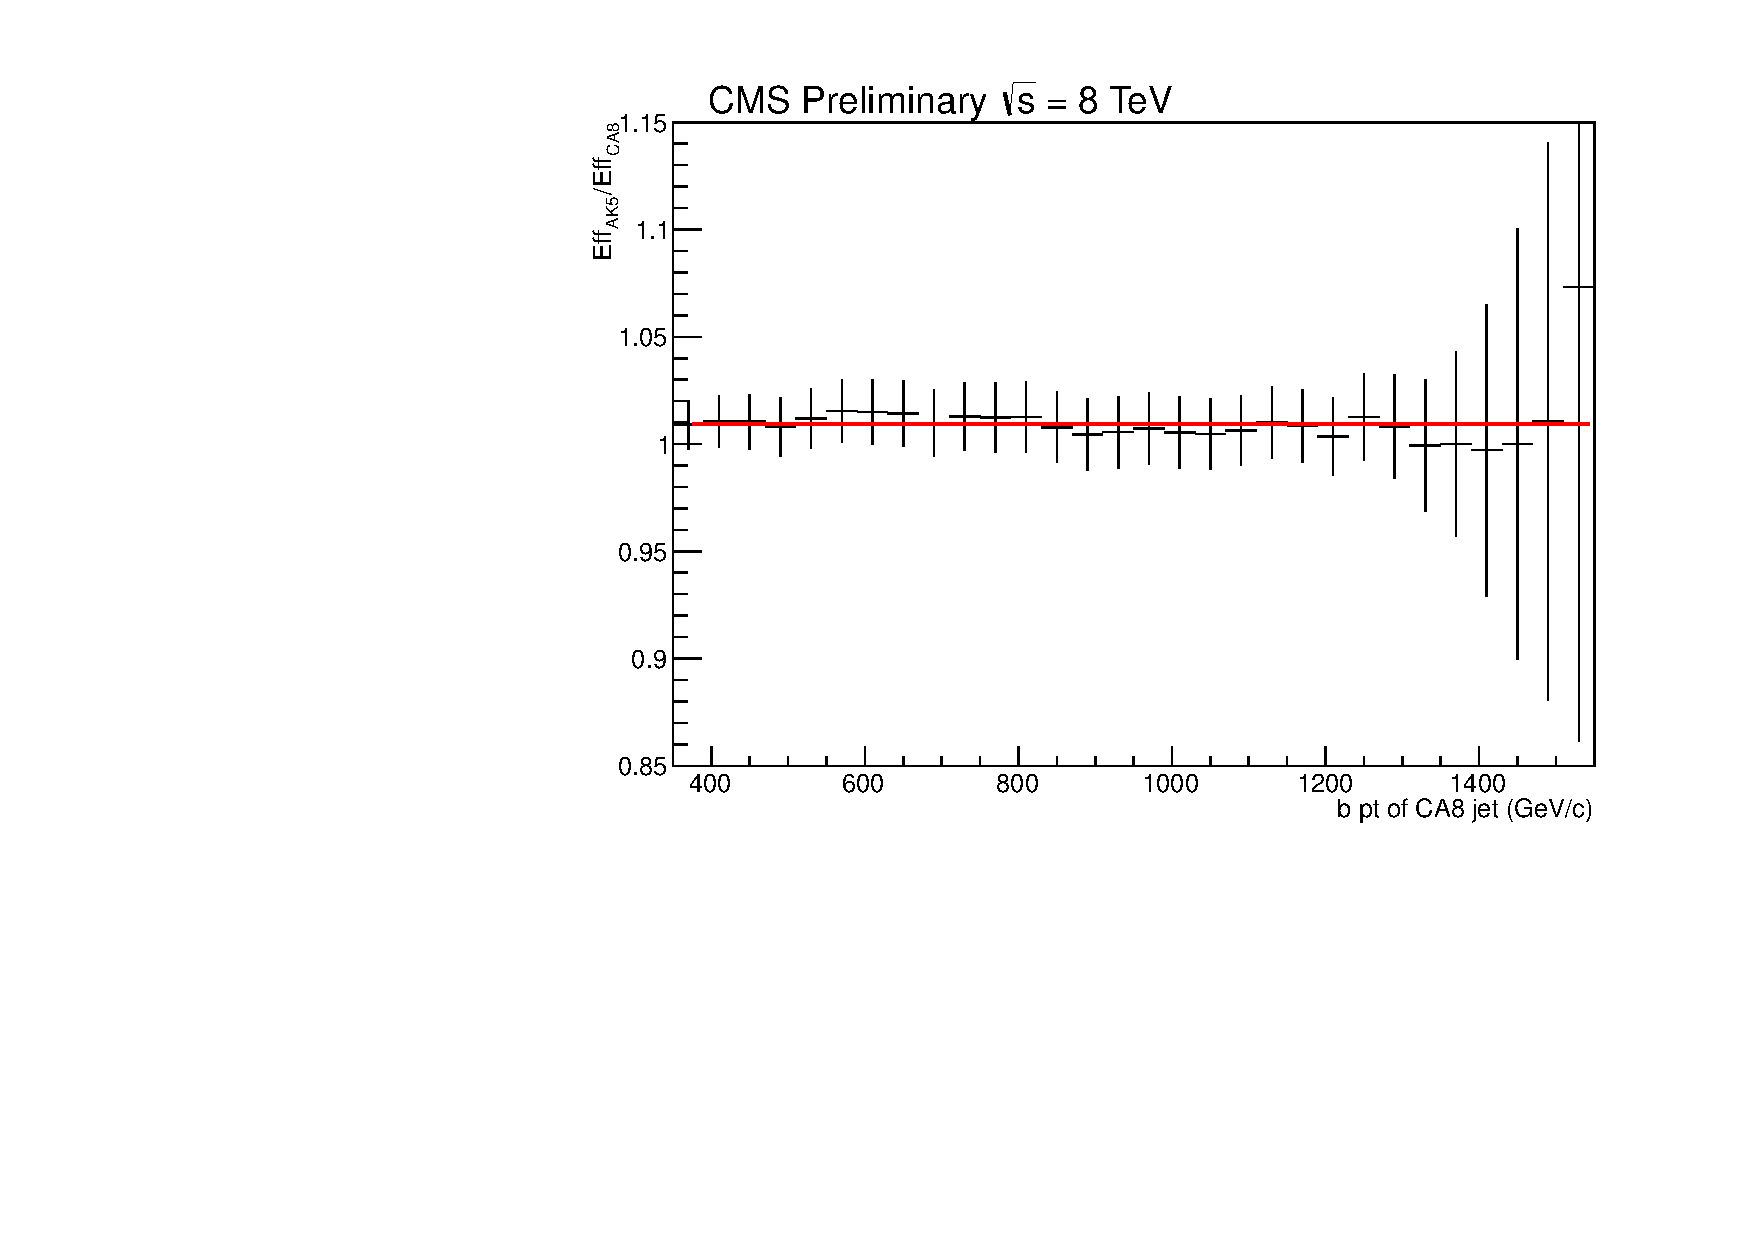
\includegraphics[width=0.9\textwidth]{AN-13-004/figs/EfficiencyCompCAptr32700.pdf}
\caption{Ratio of the AK5 b-tagging rate to the CA8 b-tagging rate. Fitting this to a constant gives us a value of 1.0098 $\pm$ 0.0031.  This can 
be considered an upper limit on the uncertainty for the change in $\mathrm{SF_b}$ for CA8 jets}

\label{figs:btageff}
\end{figure}

After the full top tagging selection is complete, there is a substantial fraction of $\ttbar$ in the full selection.
Additionally, there is a large uncertainty in the $\ttbar$ MC contribution, so discriminating signal from $\ttbar$ becomes important.  
In $\wpr$ signal MC, the sub-leading b candidate jet is usually a true b jet, but in $\ttbar$ this jet is commonly a merged W or top jet. 
To this effect, the b candidate jet is required to have a mass $\mathrm{M_b} < 70~\GeV$ in the full selection.  The value for this cut is set near the peak of the Signal/$\sqrt{\text{Background}}$ distribution (see Figure \ref{figs:BmassCOMP}).


\begin{figure}[htcb]
\begin{center}
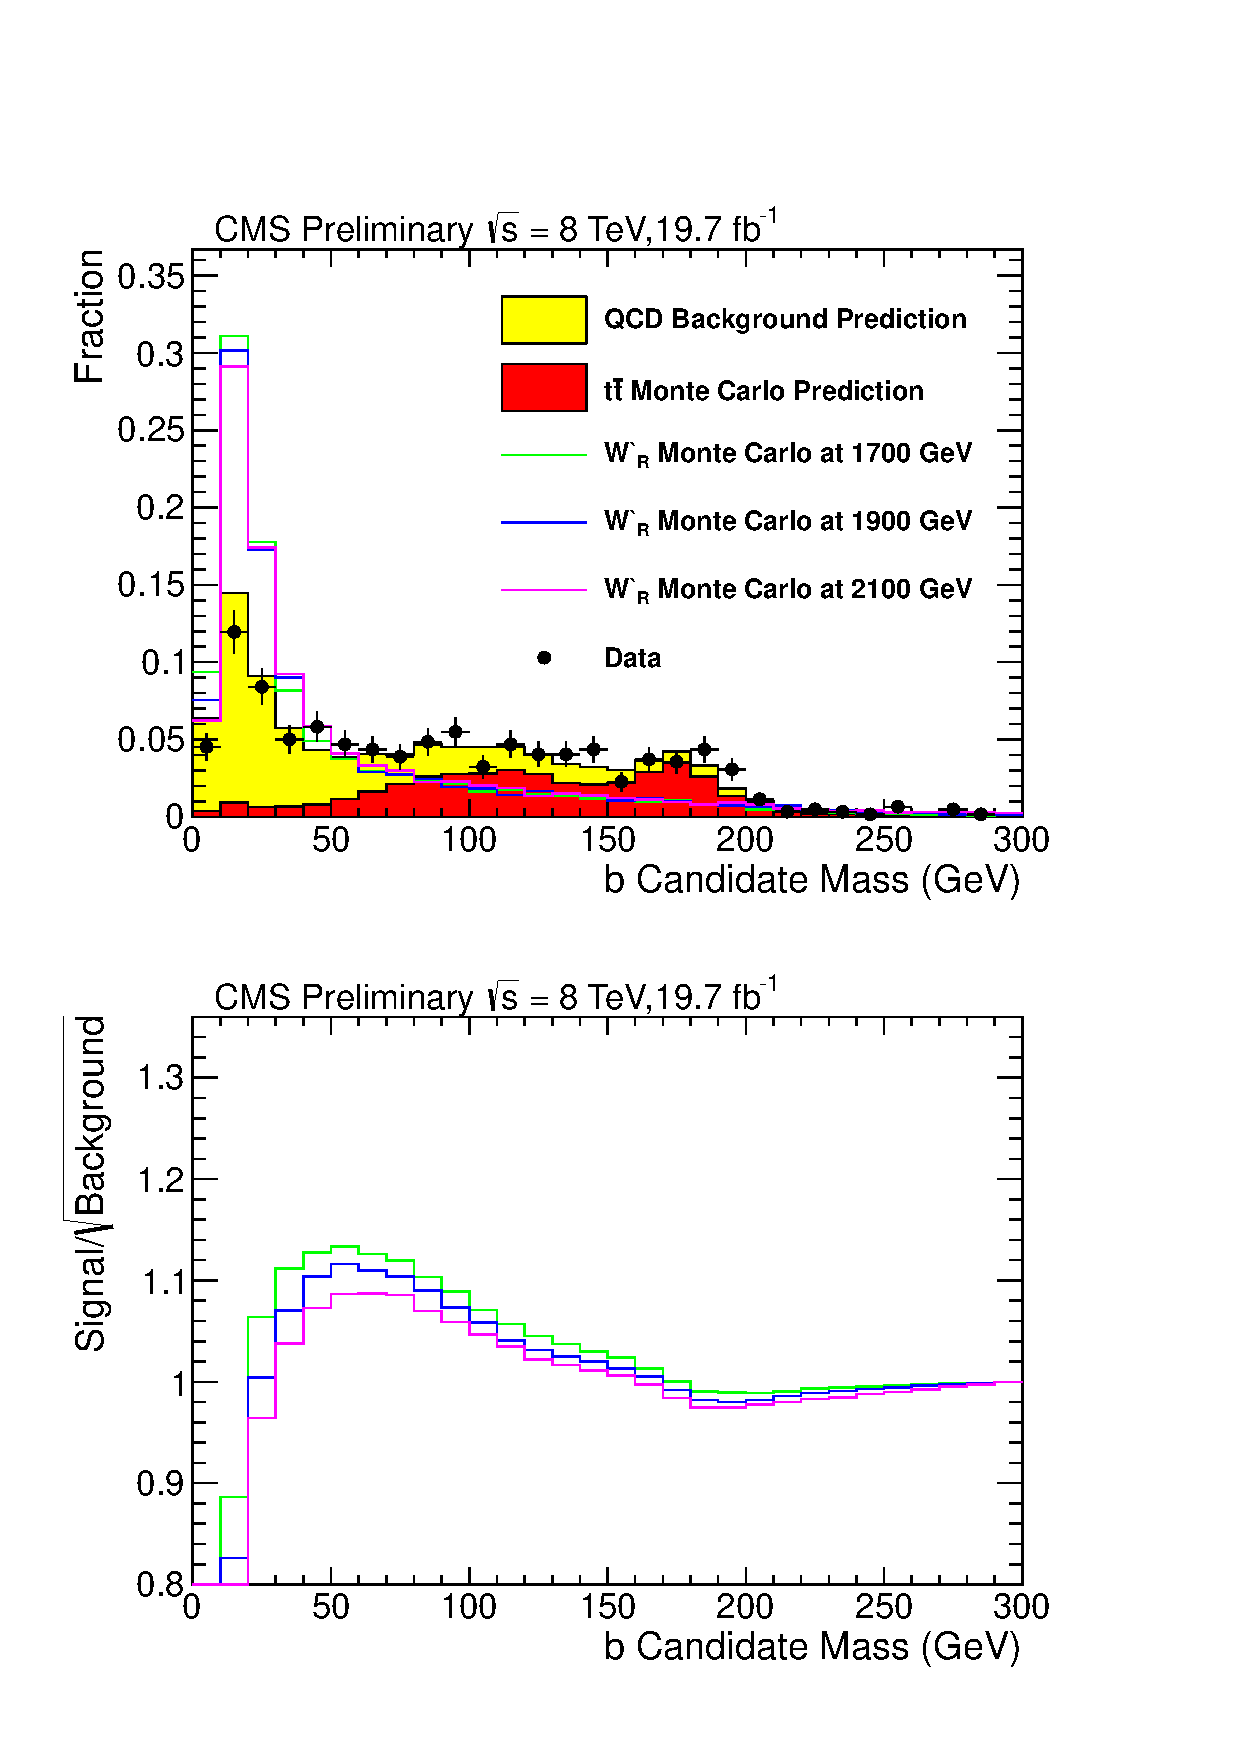
\includegraphics[width=0.7\textwidth]{AN-13-004/figs/bmassdatatosigwithdata.pdf}
\caption{
b candidate mass distributions in data, background, and signal.  Plot of Signal/$\sqrt{\text{Background}}$ (bottom), derived from the top plot. 
This plot includes the full top tagging selection using the background estimation procedure outlined in Section \ref{sec:backgroundEstimation}.
}
\label{figs:BmassCOMP}
\end{center}
\end{figure}


\subsection{Reconstruction of W' Invariant Mass}
\label{sec:fullselection}
The full selection for the reconstruction of the $\wpr$ invariant mass then includes the following offline cuts.
\begin{itemize}
\item One jet with $\pt > 450~\GeV$ identified with the CMS top tagging algorithm as well as subjet b-tagging and N-subjettiness discrimination.
\item One jet with $\pt > 370~\GeV$ with a CSVM b tag and mass$ < 70~\GeV$
\item $|\Delta \phi| > \pi/2$ between the two jets
\item $|\Delta y|$ between the two jets $<$ 1.6 
\end{itemize}
The cutflow for this selection in data, $\ttbar$ MC, and right-handed $\wpr$ signal MC can be found in Table \ref{table:Cutflow}.
Figure \ref{figs:GCFS} shows this full selection in signal MC for various $\wpr$ masses.  



\begin{sidewaystable}
\begin{center}
\begin{small}

\scalebox{0.7}{
\begin{tabular}{c||c|c|c|c|c|c|c|c|c|c}
\multicolumn{7}{c}{Number of Selected Events} \\
\hline\hline
\bf{Sample} & \bf{$2 jets$} & \bf{$\pt$} & \bf{$|\Delta y|$} & \bf{$M_{top}$} & \bf{$Nsubjets$} &  \bf{$Minmass$}  & $SJ_{\text{CSVMAX}}$  & $\mathrm{\tau_3/\tau_2}$ & $M_{b}$ & \bf{$CSV$}\\
\hline\hline
Data & 13854873$\pm$3722 & 4305244$\pm$2075 & 3376771$\pm$1838 & 992949$\pm$996 & 557489$\pm$747 & 318520$\pm$564 & 50642$\pm$225 & 7200$\pm$85 & 4463$\pm$67 & 277$\pm$17\\
QCD & --- & --- & --- & --- & --- & --- & --- & --- & --- & 248$\pm$4\\
ttbar & 12185$\pm$27.3 & 4718$\pm$17.9 & 4220$\pm$16.9 & 3217$\pm$14.4 & 2742$\pm$13.3 & 2508$\pm$12.6 & 1689$\pm$10.0 & 1024$\pm$7.8 & 178$\pm$3.6 & 37$\pm$1.4\\
M($\wpr_{R}$) = 1900 & 806$\pm$1.4 & 739$\pm$1.3 & 553$\pm$1.2 & 429$\pm$1.0 & 340$\pm$0.9 & 304$\pm$0.9 & 170$\pm$0.6 & 88$\pm$0.4 & 68$\pm$0.4 & 16$\pm$0.2\\
M($\wpr_{R}$) = 2100 & 401$\pm$0.7 & 372$\pm$0.7 & 268$\pm$0.6 & 209$\pm$0.5 & 163$\pm$0.4 & 143$\pm$0.4 & 76$\pm$0.3 & 38$\pm$0.2 & 29$\pm$0.2 & 6$\pm$0.1\\
M($\wpr_{L}$) = 1900 & 796$\pm$2.4 & 703$\pm$2.3 & 531$\pm$2.0 & 414$\pm$1.8 & 312$\pm$1.6 & 274$\pm$1.5 & 138$\pm$1.0 & 58$\pm$0.6 & 44$\pm$0.6 & 10$\pm$0.3\\
M($\wpr_{L}$) = 2100 & 430$\pm$1.6 & 364$\pm$1.5 & 268$\pm$1.3 & 205$\pm$1.1 & 152$\pm$1.0 & 130$\pm$0.9 & 63$\pm$0.6 & 27$\pm$0.4 & 20$\pm$0.3 & 4$\pm$0.2\\
\hline
\end{tabular}
}
\caption{The number of selected events after successive selections as scaled to an integrated luminosity of 19.7~$\fbinv$.  Table reads left to right where the current column implies the previous selection.  The quoted uncertainty is statistical only.  QCD background expectation is only recorded for the full selection, as the average b-tagging rate takes into account the QCD background b fraction increase from b-tagging and subjet b-tagging.  
The first column additionally represents the hemispherical $\delta \phi$ selection between the leading jets.  
The column labeled $\pt$ represents the $\pt$ selection placed on both leading jets.  The signal events are normalized to theory cross-section.}
\label{table:Cutflow}
\end{small}
\end{center}
\end{sidewaystable}




%\begin{sidewaystable}
%\begin{center}
%\begin{small}
%\begin{tabular}{cccccccccc}
%\multicolumn{7}{c}{Data Cutflow} \\
%\hline\hline
%\bf{2 jets} & \bf{$\pt$} & \bf{$|\Delta y|$} & \bf{$M_{top}$} & \bf{$Nsubjets$} &  \bf{$Minmass$} & \bf{$CSV$}  & $\mathrm{\tau_3/\tau_2}$ & $M_{b}$ & $SJ_{\text{CSVMAX}}$\\
%\hline
%71.10\% & 22.04\% & 17.28\% & 5.08\% & 2.85\% & 1.63\% & 0.09\% & 0.01\% & 0.007\% & 0.001\%\\
%\end{tabular}
%\caption{Cutflow for Data. Table reads left to right where the current column implies the previous cuts}
%\vspace{1cm}

%\begin{tabular}{cccccccccc}
%\multicolumn{7}{c}{$\ttbar$ Cutflow} \\
%\hline\hline
%\bf{2 jets} & \bf{$\pt$} & \bf{$|\Delta y|$} & \bf{$M_{top}$} & \bf{$Nsubjets$} &  \bf{$Minmass$} & \bf{$CSV$}  & $\mathrm{\tau_3/\tau_2}$ & $M_{b}$ & $SJ_{\text{CSVMAX}}$\\
%\bf{2 jets $\pt > 150$} & \bf{Jet1 $\pt > 450$ ; Jet2 $\pt > 370$} & %\bf{$|\Delta y| < 1.6$} & \bf{$140 < M_{top} < 250$} & \bf{$Nsubjets > 2$} &  %\bf{$Minmass > 50$} & \bf{$CSV > 0.679$} & $\tau_3/\tau_2 <0.55$ & $Jet2 Mass < 70$ & $SJ_{\text{CSVMAX}} > 0.679$  \\
%\hline
%26.50\% & 0.91\% & 0.82\% & 0.62\% & 0.52\% & 0.47\% & 0.12\% & 0.06\% & 0.009\% & 0.007\%\\
%\end{tabular}
%\caption{Cutflow for TTbar MC. Table reads left to right where the current column implies the previous cuts}
%\vspace{1cm}

%\begin{tabular}{c|cccccccccc}
%\multicolumn{8}{c}{Signal Cutflow} \\
%\hline\hline
%\bf{$M_{\wpr}$} & \bf{2 jets $\pt > 150$} & \bf{Jet1 $\pt > 450$ ; Jet2 $\pt > 370$} & \bf{$|\Delta y| < 1.6$} & \bf{$140 < M_{top} < 250$} & \bf{$Nsubjets > 2$} &  \bf{$Minmass > 50$} & \bf{$CSV > 0.679$} & $\tau_3/\tau_2 <0.55$ & $Jet2 Mass < 70$ & $SJ_{\text{CSVMAX}} > 0.679$ \\
%\bf{$M_{\wpr}$} & \bf{2 jets} & \bf{$\pt$} & \bf{$|\Delta y|$} & \bf{$M_{top}$} & \bf{$Nsubjets$} &  \bf{$Minmass$} & \bf{$CSV$}  & $\mathrm{\tau_3/\tau_2}$ & $M_{b}$ & $SJ_{\text{CSVMAX}}$\\
%\hline
%1300 & 77.86\% & 44.33\% & 42.09\% & 27.24\% & 22.55\% & 20.31\% & 7.19\%& 3.79\%& 3.08\%& 2.16\%\\
%1500 & 78.25\% & 52.64\% & 45.20\% & 32.66\% & 26.69\% & 24.15\% & 7.42\%& 3.74\%& 2.95\%& 2.02\%\\
%1700 & 78.01\% & 57.37\% & 45.44\% & 34.47\% & 27.59\% & 24.92\% & 6.67\%& 3.22\%& 2.49\%& 1.68\%\\
%1900 & 77.20\% & 59.36\% & 44.40\% & 34.51\% & 27.19\% & 24.26\% & 5.74\%& 2.72\%& 2.06\%& 1.34\%\\
%2100 & 76.04\% & 59.72\% & 42.95\% & 33.56\% & 26.05\% & 22.70\% & 4.87\%& 2.20\%& 1.63\%& 1.02\%\\
%2300 & 74.20\% & 58.37\% & 40.87\% & 31.80\% & 24.63\% & 20.70\% & 4.14\%& 1.87\%& 1.37\%& 0.84\%\\
%2700 & 69.36\% & 51.81\% & 35.51\% & 27.13\% & 21.51\% & 16.32\% & 3.06\%& 1.34\%& 0.99\%& 0.61\%\\
%3100 & 63.12\% & 40.89\% & 28.57\% & 21.23\% & 17.34\% & 12.28\% & 2.54\%& 1.15\%& 0.86\%& 0.55\%\\
%\end{tabular}
%\caption{Cutflow for Right-Handed $\wpr$ signal MC. Table reads left to right where the current column implies the previous cuts}
%\label{table:Cutflows}
%\end{small}
%\end{center}
%\end{sidewaystable}

\begin{figure}[htcb]
\begin{center}
\subfigure{\label{figs:GCFSright}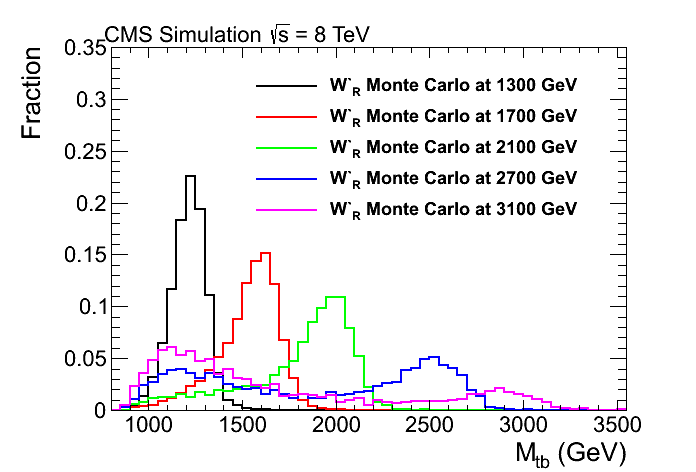
\includegraphics[width=0.45\textwidth]{AN-13-004/figs/SignalMCFScomparison}}\\
\subfigure{\label{figs:GCFSleft}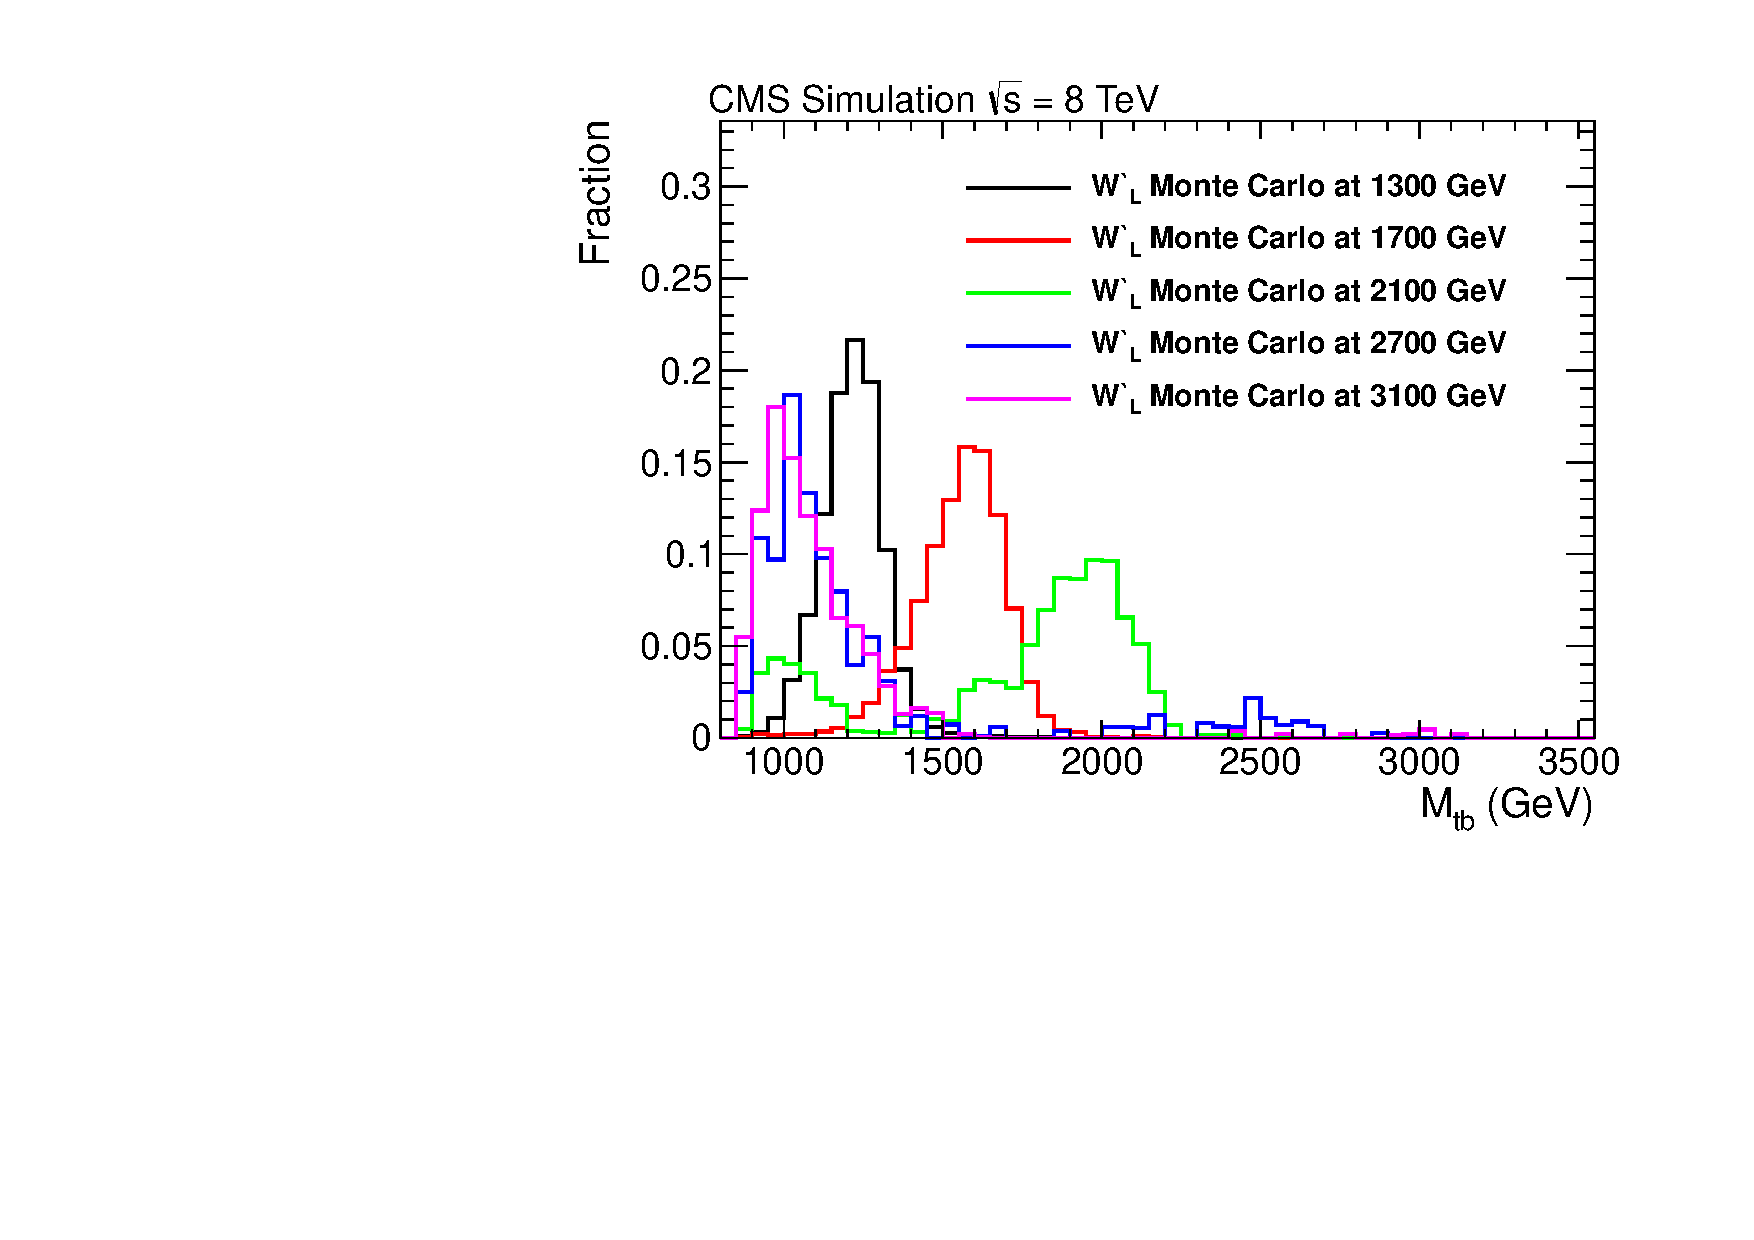
\includegraphics[width=0.45\textwidth]{AN-13-004/figs/SignalLeftMCFScomparison.pdf}}
\subfigure{\label{figs:GCFSmixed}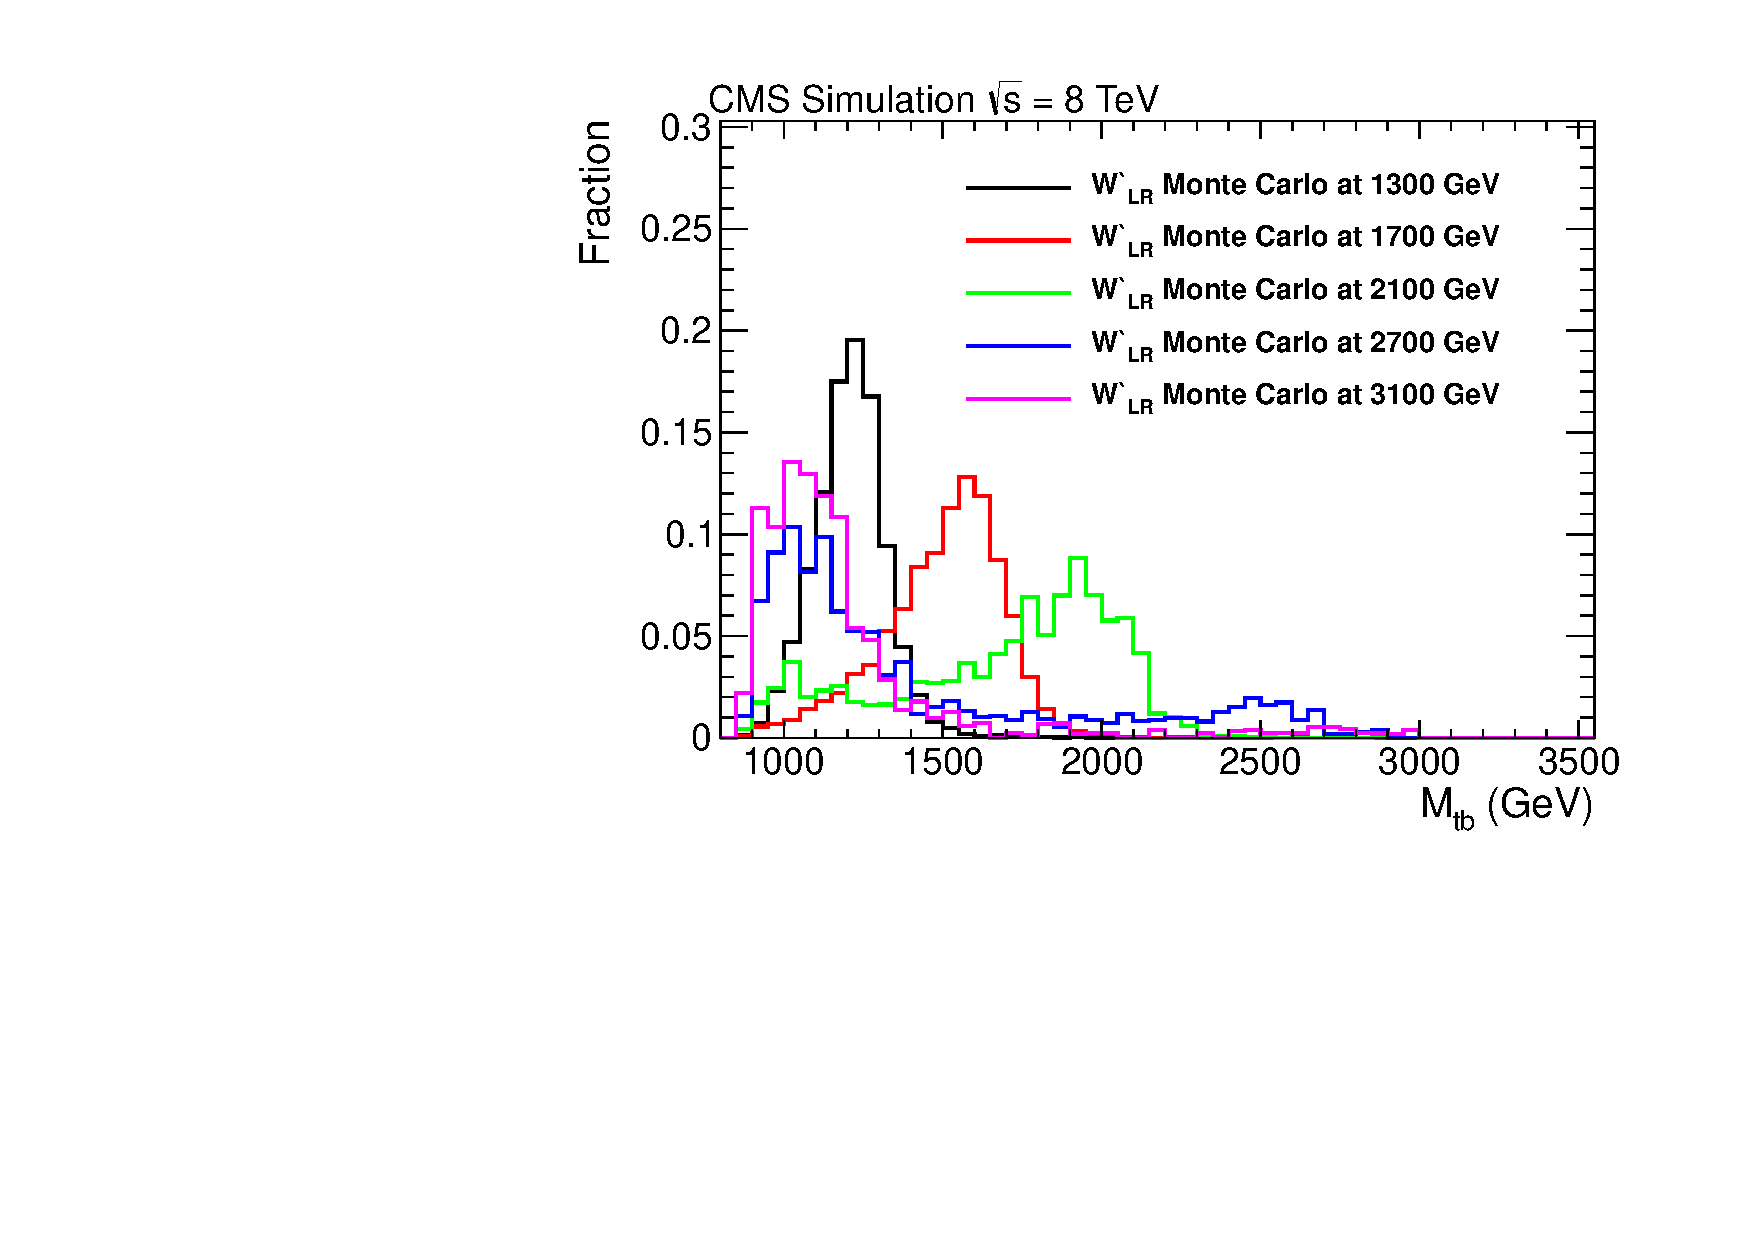
\includegraphics[width=0.45\textwidth]{AN-13-004/figs/SignalMixedMCFScomparison.pdf}}
\caption{
Full selection applied to $\wpr_{R}$ (top) $\wpr_{L}$ (bottom-left) and $\wpr_{LR}$ (bottom-right).  The bimodal structure seen in the $\mathrm{M_{tb}}$ spectrum for high $\wpr$ mass is a feature common to high-mass large-width resonances and represents the superposition of a $\wpr$ resonance and a rapidly falling parton distribution function. 
}
\label{figs:GCFS}
\end{center}
\end{figure}

%\begin{figure}[htcb]
%\centering
%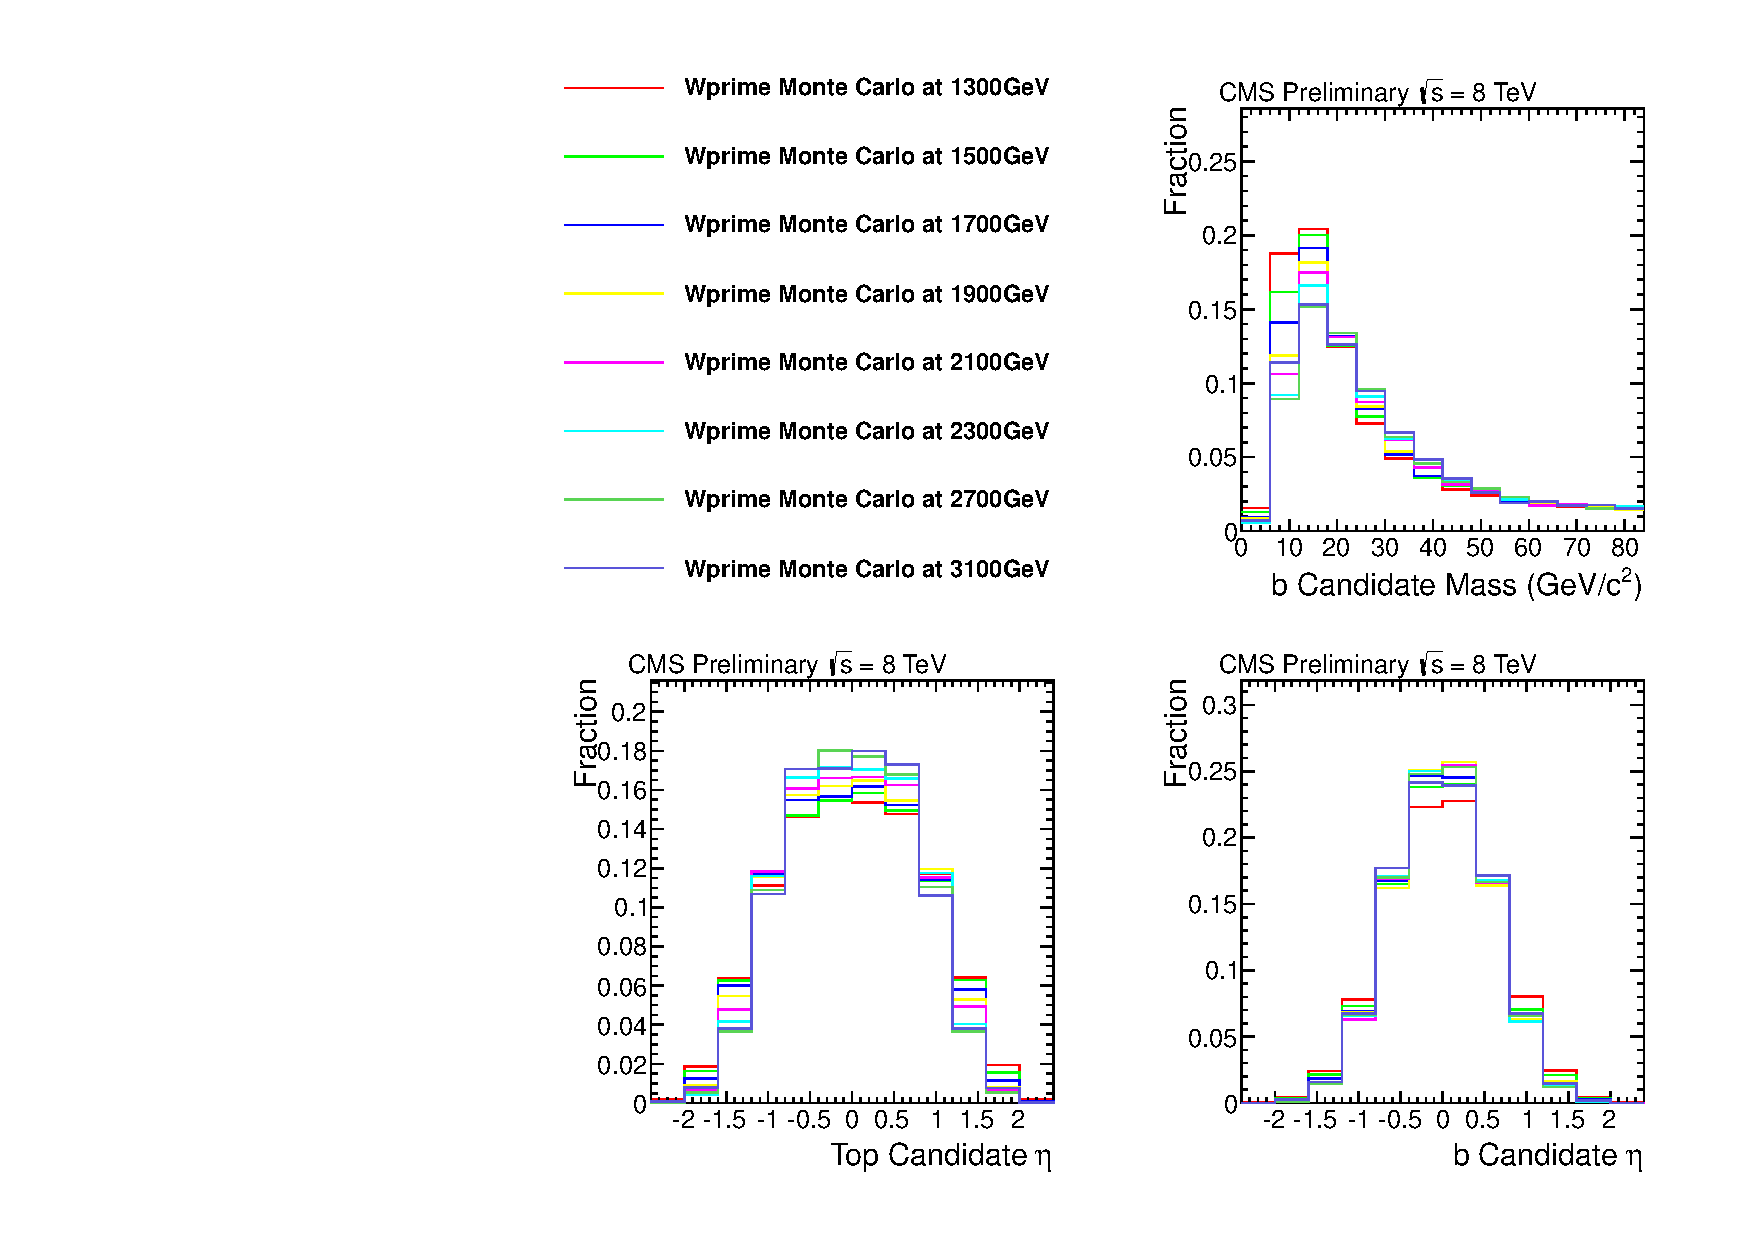
\includegraphics[width=0.9\textwidth]{AN-13-004/figs/KinPlots_Signal1}
%\caption{Full selection in right-handed $\wpr$ signal MC kinematic distributions}
%\label{figs:kinplotssignal1}
%\end{figure}

%\begin{figure}[htcb]
%\centering
%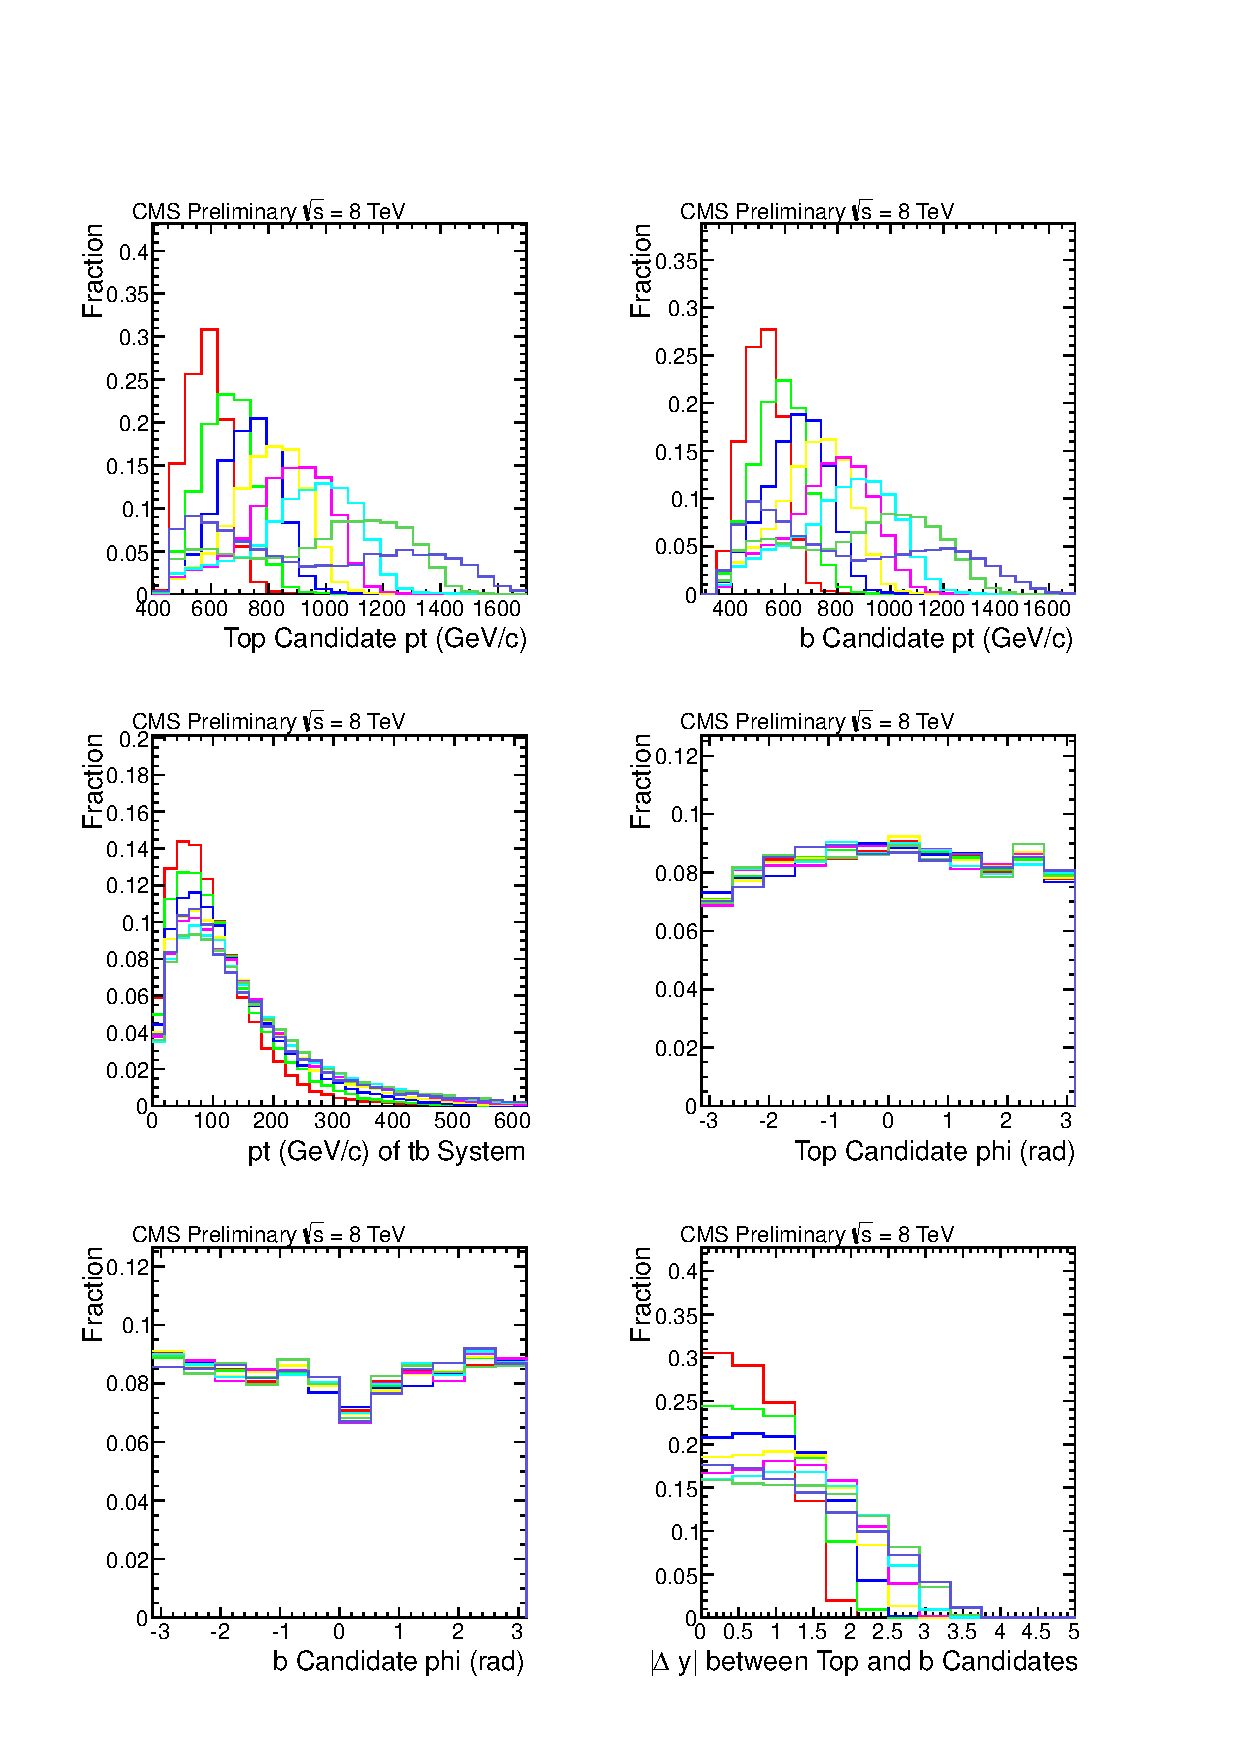
\includegraphics[width=0.9\textwidth]{AN-13-004/figs/KinPlots_Signal2}
%\caption{Full selection in right-handed $\wpr$ signal MC kinematic distributions}
%\label{figs:kinplotssignal2}
%\end{figure}
\clearpage
